%!TeX root=../thesisStructure.tex
% Chapter 2
\chapter{Desarrollo y Resultados} % Chapter title
\label{ch:MarcoTeorico} 

\section{Recolección de muestras del proceso de potabilización}

Para poder iniciar con la tarea de recolección de muestras en la planta de potabilización, primero era necesario conocer los puntos en los cuales las muestras serían tomadas. Por lo tanto, tomando en cuenta las recomendaciones 
dadas por los especialistas de la planta de tratamiento y los resultados de trabajos previos realizados en esa instalación, se determinó que los puntos de agua cruda, tanque de mezclado rápido, canal sedimentador, salida 
de los filtros y la salida de agua potable serían las fases consideradas para muestreo.

Referente a la elección de las 5 etapas para muestreo, es evidente que el análisis de la entrada del proceso, agua cruda, es fundamental para tener la referencia inicial de los parámetros de calidad para líquido con nulo 
tratamiento, lo cual nos permite conocer las condiciones iniciales y así observar cómo los parámetros cambian gradualmente durante el proceso. Posteriormente, se eligen 3 etapas intermedias del proceso que no sean subsecuentes,
lo cual es importante para que los cambios en la calidad del agua sea de mayor magnitud. Además, la importancia de tener registro completo de los cambios en la calidad del agua entre la entrada y salida del proceso. Finalmente, 
la base de datos generada debe tener registro de la calidad en el producto final del proceso, lo cual permite completar la caracterización de las variables de calidad que se estarán analizando.

La obtención de muestras de agua se ha realizado directamente en la planta de potabilización en las etapas específicas del proceso determinadas previamente. Esta recolección de muestras de líquido desde la planta se realizó 
a lo largo del año 2024, dividiendo temporalmente los muestreos para las diferentes estaciones del año, con el fin de tener evidencia para los diferentes tipos de clima que se presentan.

La medición de las muestras recolectadas inicialmente se llevó a cabo en los laboratorios del ITM después de que se realizaba el traslado de las muestras desde la planta. Posteriormente, las mediciones se comenzaron a llevar 
a cabo en el laboratorio de muestreo de la planta de potabilización. Para la medición de los diferentes parámetros considerados durante el proyecto, se estuvo haciendo uso del equipo de medición Pool Kit junto con los diferentes 
sensores del mismo fabricante Atlas Scientific para cada variable individual. Adicionalmente, en el laboratorio de muestreo del OOAPAS también se nos permitió uso de su equipo de medición para realizar mediciones puntuales 
en casos en los cuales no era posible el uso de nuestro equipo.

La primera caracterización del proceso de potabilización se realizó en enero de 2024. Esta primera caracterización fue llevada a cabo con muestras recolectadas previamente, de las cuales 
se obtuvieron pequeñas cantidades correspondientes a las etapas específicas. En esta caracterización los parámetros medidos fueron ORP, temperatura, pH y conductividad; para cada una de las 5 muestras 
se realizaron 3 mediciones, cada una de ellas de una duración aproximada de entre 15 y 20 minutos. Es decir, primeramente se introducen los sensores a la muestra de agua durante el tiempo determinado, posteriormente se 
sacan para enjuagarlos y limpiarlos con agua destilada, para posteriormente volver a introducirlos durante el tiempo establecido. 

Al mismo tiempo que se realiza la medición de las muestras, los datos registrados por los sensores se almacenan y etiquetan en archivos de tipo CSV. Particularmente para este primer experimento, los datos recolectados no han 
podido ser considerados confiables debido a que las muestras medidas tenían varíos días de haberse recolectado de la planta, lo que genera su deterioro y la pérdida de sus propiedades y características que se 
busca analizar. Por lo cual es importante que las mediciones se realicen sin dejar pasar mucho tiempo una vez que las muestras son extraídas en la planta.


%\tikzstyle{startstop} = [rectangle, rounded corners, 
						%minimum width=3cm, 
						%minimum height=1cm,
						%text centered, 
						%draw=black, 
						%fill=red!30]

%\tikzstyle{io} = [trapezium, 
				  %trapezium stretches=true, % A later addition
				  %trapezium left angle=70, 
				  %trapezium right angle=110, 
				  %minimum width=3cm, 
				  %minimum height=1cm, text centered, 
				  %draw=black, fill=blue!30]

%\tikzstyle{process} = [rectangle, 
					   %minimum width=3cm, 
					   %minimum height=1cm, 
					   %text centered, 
					   %text width=3cm, 
					   %draw=black, 
					   %fill=orange!30]

%\tikzstyle{decision} = [diamond, 
						%minimum width=3cm, 
						%minimum height=1cm, 
						%text centered, 
						%draw=black, 
						%fill=green!30]
%\tikzstyle{arrow} = [thick,->,>=stealth]

%\begin{center}
%\begin{tikzpicture}[node distance=2cm]

	%\centering

	%\node (start) [startstop] {\textbf{AGUA CRUDA}};
	%\node (in1) [process, below of=start,yshift=-0.2cm] {COAGULACIÓN Y FLOCULACIÓN};
	%\node (pro1) [process, below of=in1,yshift=-0.2cm] {CASETA DE CLORACIÓN};
	%\node (dec1) [startstop, below of=pro1, yshift=-0.2cm] {\textbf{TANQUE DE MEZCLA RÁPIDA}};
	%\node (indz100) [process, below of=dec1, yshift=-0.2cm] {TANQUE DE MEZCLA LENTA};
    %\node (indz101) [startstop, below of=indz100, yshift=-0.2cm] {\textbf{CANAL SEDIMENTADOR}};
	%\node (indz102) [process, below of=indz101, yshift=-0.2cm] {FILTROS};
	%\node (indz103) [startstop, below of=indz102, yshift=-0.2cm] {\textbf{SALIDA DE FILTROS}};
	%\node (indz104) [process, below of=indz103, yshift=-0.2cm] {TANQUE DE ALMACENAMIENTO};
	%\node (indz105) [startstop, below of=indz104, yshift=-0.2cm] {\textbf{AGUA POTABLE}};	
														   
%\end{tikzpicture}
%\end{center}

Finalmente, en la primera caracterización del proceso se ha establecido la metodología de medición que se llevará a cabo para los siguientes muestreos. Básicamente esta parte está relacionada con los cuidados que se debe tener 
en el manejo de las muestras de agua y del equipo de medición. En cuanto al manejo de las muestras de agua, la parte fundamental es la limpieza necesaria en los frascos donde se recolecta el líquido para evitar contaminación 
de las muestras. En lo referente al equipo de medición, el cuidado especial igualmente es sobre la limpieza y enjuague de los sensores al cambiar entre muestras de diferentes etapas para evitar muestras contaminadas. 

En la segunda caracterización del proceso de potabilización, llevada a cabo en el mes de febrero, se miden las variables de temperatura, pH, ORP y conductividad. En este segundo experimento las mediciones fueron efectuadas 
en un periodo de tiempo de 4 días, y para este segundo muestreo dicho factor ha sido por el cual se nos ha hecho la recomendación de efectuar las mediciones el mismo día que las muestras son extraídas, y en caso de tardar 
más de 1 día, es recomendable refrigerar las muestras para evitar su deterioro.

La tercera caracterización se efectuó el día 6 de marzo de 2024 y los parámetros medidos fueron temperatura, pH, ORP y conductividad. La recolección de las muestras 
se realizó 1 día antes, el 5 de marzo por la tarde, y la totalidad de las mediciones se efectuaron el dia siguiente, teniendo en esta ocasión una duración aproximada de 40 minutos 
de monitoreo para cada 1 de las 5 muestras recolectadas. En esta tercera caracterización el cambio importante efectuado durante el monitoreo de las muestras fue el orden en que se hacían las mediciones. A partir de este 
experimento y para los siguientes se definió que las mediciones se harían en el orden inverso al avance dado por el proceso, es decir, la primera medición se hace sobre la muestra de agua potable, en segundo 
lugar la muestra de salida de filtración, en tercer lugar la muestra de canal sedimentador, posteriormente la muestra de tanque de mezclado rápido, y por último la muestra de agua cruda. 

La conclusión para la tercera caracterización ha sido sobre el descarte de las variables de temperatura, pH y conductividad para modelos de clasificación. Esta determinación se ha hecho tomando como referencia resultados 
estadísticos que se presentan en la sección siguiente de este capítulo.

La cuarta caracterización fue llevada a cabo los días 12 y 13 de marzo de 2024, siendo las etapas de agua potable y salida de filtración caracterizadas el primer día por la tarde y las 3 etapas anteriores medidas por la 
mañana del 13 de marzo; para este experimento se dejaron de considerar los parámetros de pH y conductividad eléctrica, y se agregó al equipo Pool Kit un sensor de oxígeno disuelto, además de que en el laboratorio de muestreo 
del OOAPAS nos proporcionaron los datos puntuales para el parámetro de cloro residual. 

Los resultados finales de la cuarta caracterización entregaron los comportamientos esperados tanto para los parámetros que ya se tenían como para los parámetros incluidos en este experimento. Principalmente en el caso de 
cloro residual, en las primeras 3 etapas, agua cruda, tanque de mezcla rápida y canal sedimentador, no hubo presencia. Fue hasta las 2 útimas etapas, salida de filtros y agua potable, que ya pudo detectar 
la presencia de remanentes del agente desinfectante.

La quinta caracterización se llevó a cabo los días 23 y 24 de abril, teniendo que las etapas de agua potable y salida de filtración se midieron la tarde del primer día, y las etapas de agua cruda, tanque de mezclado rápido 
y canal sedimentador se caracterizaron el segundo día por la mañana. Las variables medidas en este experimento fueron temperatura, oxígeno disuelto y ORP; el parámetro de cloro residual no pudo obtenerse ya que 
en el laboratorio de calidad del agua en el OOAPAS no hubo disponibilidad de que se nos proporcionara esa información. Adicionalmente, en este quinto experimento el tiempo de medición fue aproximadamente de 40 minutos para 
cada 1 de las 5 muestras.

La quinta caracterización entregó resultados importantes sobre la variable de oxígeno disuelto que derivaron en decisiones sobre un cambio significativo en la metodología de trabajo. Al final de este quinto experimento, 
los rangos de valores para oxígeno disuelto en las distintas etapas no presentaron una tendencia que permitiera diferenciar claramente las etapas del proceso con el uso de este parámetro. Por lo tanto, en este momento se decidió 
trasladar el equipo de instrumentación al laboratorio de muestreo del OOAPAS, ya que hasta este punto los monitoreos se hacían después de que las muestras de agua eran extraídas 
de la planta y posteriormente trasladadas al laboratorio de posgrado del Tecnológico. Esto permite evitar cambios no deseados en los parámetros analizados, ya que dichos parámetros son afectados por los cambios de 
temperatura.

Para la sexta caracterización, la fecha de realización corresponde al día 02 de julio de 2024. Para las muestras recolectadas ahora las mediciones se han llevado a cabo en el laboratorio de muestreo 
en la planta de potabilización. Referente a las diferencias que se pueden observar en los datos recolectados ahora que la caracterización
se realiza inmediatamente después de la recolección de la muestras, por ejemplo, está el caso del oxígeno disuelto. Para este parámetro se tiene el siguiente problema. Cuando en un recipiente o frasco como los que se usan 
en esta investigación para la recolección de las muestras, estos frascos contienen el agua de una fase específica y al mismo tiempo el líquido contenido conserva el oxígeno disuelto 
que ha ido atrapando en su recorrido. Sin embargo, que el agua contenida en los frascos pueda retener el oxígeno disuelto en ella, depende de la solubilidad de dicho gas, la cual a su vez depende de las condiciones de temperatura 
y presión a las que se encuentra la muestra. 

Es decir, se puede mantener los frascos cerrados y conservar el mismo valor de presión en la muestra, pero en el traslado de las muestras de la planta de potabilización al laboratorio 
del ITM se genera un aumento de temperatura. Es aquí donde existe un problema con el oxígeno disuelto; un aumento de temperatura en una muestra contenida en un 
frasco en esas condiciones, generará un descenso en la solubilidad del gas oxígeno existente en el agua.
Por lo tanto, si la caracterización de las muestras se hace una vez que se han llevado al laboratorio de posgrado, los valores medidos para oxígeno disuelto serán menores en comparación con las condiciones reales, ya que 
el aumento de temperatura genera descenso en la solubilidad del oxígeno en el agua, lo cual genera una pérdida de dicho gas una vez que los frascos son abiertos. 

Para esta sexta caracterización, se realizaron 3 muestreos el mismo día; el primero, a las 9 de la mañana; el segundo, a la 1 de la tarde; el tercero, a las 5 de la tarde. Para esta fecha en la que se realiza esta sexta 
caracterización, ya la ciudad de Morelia se encuentra en época de lluvias, por lo cual se generan escurrimientos los cuales contienen una gran cantidad de contaminantes, los cuales se mezclan con el agua que llega a la planta
para su tratamiento; entre los contaminantes que se pueden agregar se encuentran por ejemplo todo lo que se arrastra por el suelo, tanto subterráneo como lo que se encuentra sobre las carreteras, tales como aceite de automóviles,
químicos fertilizantes o la simple mezcla de lodo que escurre de las montañas y se incorpora al agua que llega a la planta de potabilización. Es importante tener en cuenta que la época de lluvias termina aproximadamente a 
mediados de octubre, por lo cual las caracterizaciones realizadas a partir de esta fecha y hasta el final de la época de lluvias, será importante tener ciertas consideraciones sobre efectos no deseados en los valores para 
los datos recolectados. 

En la \autoref{tab:table20000_1} se muestran los coeficientes de correlación para los datos del sexto experimento.

\begin{table}[h]
	\begin{center}
		\begin{tabular}{| c | c | c | c | c | c |}
			\hline
			\multicolumn{6}{ |c| }{Matriz de correlación Pearson} \\ \hline
			 & Temperatura & DO & ORP & Conductividad & Cloro Residual \\ \hline
			 Temperatura & 1 & 0.7564 & 0.7279 & 0.1051 & 0.4286 \\
			 DO & 0.7564 & 1 & 0.823 & -0.0069 & 0.6775 \\
			 ORP & 0.7279 & 0.823 & 1 & -0.1727 & 0.6874 \\
			 Conductividad & 0.1051 & -0.0069 & -0.1727 & 1 & -0.2738 \\ 
			 Cloro Residual & 0.4286 & 0.6775 & 0.6874 & -0.2738 & 1 \\ \hline
			 \multicolumn{6}{ |c| }{Matriz de correlación Spearman} \\ \hline
			 & Temperatura & DO & ORP & Conductividad & Cloro Residual \\ \hline
			 Temperatura & 1 & 0.7268 & 0.7567 & 0.3267 & 0.4093 \\
			 DO & 0.7268 & 1 & 0.8167 & 0.0349 & 0.7184 \\
			 ORP & 0.7567 & 0.8167 & 1 & 0.0041 & 0.7093 \\
			 Conductividad & 0.3267 & 0.0349 & 0.0041 & 1 & -0.1939 \\
			 Cloro Residual & 0.4093 & 0.7184 & 0.7093 & -0.1939 & 1 \\ \hline
		\end{tabular}
		\caption{Coeficientes de correlación para la sexta caracterización}
		\label{tab:table20000_1}
	\end{center}
\end{table}

En la \autoref{tab:table20000_1} se observa que los coeficientes de correlación son altos para los parámetros de ORP, cloro residual y oxígeno disuelto. Esto implica que los cambios en la metodología en la toma de mediciones 
ha generado resultados más cercanos a lo establecido en la teoría.

La séptima caracterización fue realizada el día 04 de julio de 2024 y los parámetros significativos medidos fueron oxígeno disuelto, ORP y cloro residual. Al igual que para la sexta caracterización, nuevamente 
se hizó 3 veces la recolección de muestras en horarios establecidos; 9 de la mañana, primera recolección; 1 de la tarde, segunda recolección; 5 de la tarde, la tercera muestra. Igualmente, el análisis de las muestras se llevó 
a cabo en el laboratorio de muestreo de la planta de potabilización. 

La octava caracterización se llevó a cabo el día 09 de julio de 2024 y los parámetros significativos monitoreados fueron de nuevo ORP, cloro residual y oxíegno disuelto. Para este octavo experimento, se pidió 
un cambio en la metodología específicamente para esta caracterización, ya que se buscaba hacer un análisis acerca de si para este proceso de potabilización los parámetros  que se están estudiando tienen 
variaciones rápidas a lo largo del día. Lo que se pidió fue realizar recolección de muestras del proceso cada 2 horas durante el transcurso de este día, y medir las variables para poder determinar 
si existiesen variaciones significativas de los parámetros en el rango de tiempo de 1 día. En esta ocasión sólo se recolectaron muestras de 2 etapas del proceso, tanque de mezcla rápida y agua potable, debido a que no se contaba 
con el tiempo necesario para medir las 5 etapas en un rango de tiempo de 2 horas. Los horarios de recolección de muestras se plantearon que 
fuesen a las 10 de la mañana, 12 de la tarde, 2 de la tarde, 4 de la tarde y 6 de la tarde, sin embargo, la última recolección no se pudo ejecutar debido a las condiciones de lluvia.

Para el caso de la variable de ORP en la etapa de tanque de mezcla rápida, se muestran los resultados de los datos medidos en la \autoref{fig:figura1000_4}, \autoref{fig:figura1000_5}, \autoref{fig:figura1000_6} y \autoref{fig:figura1000_7}.
En los ejes horizontales se tiene el número de muestras y la magnitud de la variable se encuentra en el eje vertical de las gráficas.

\clearpage

\begin{figure}[h]
	\centering
	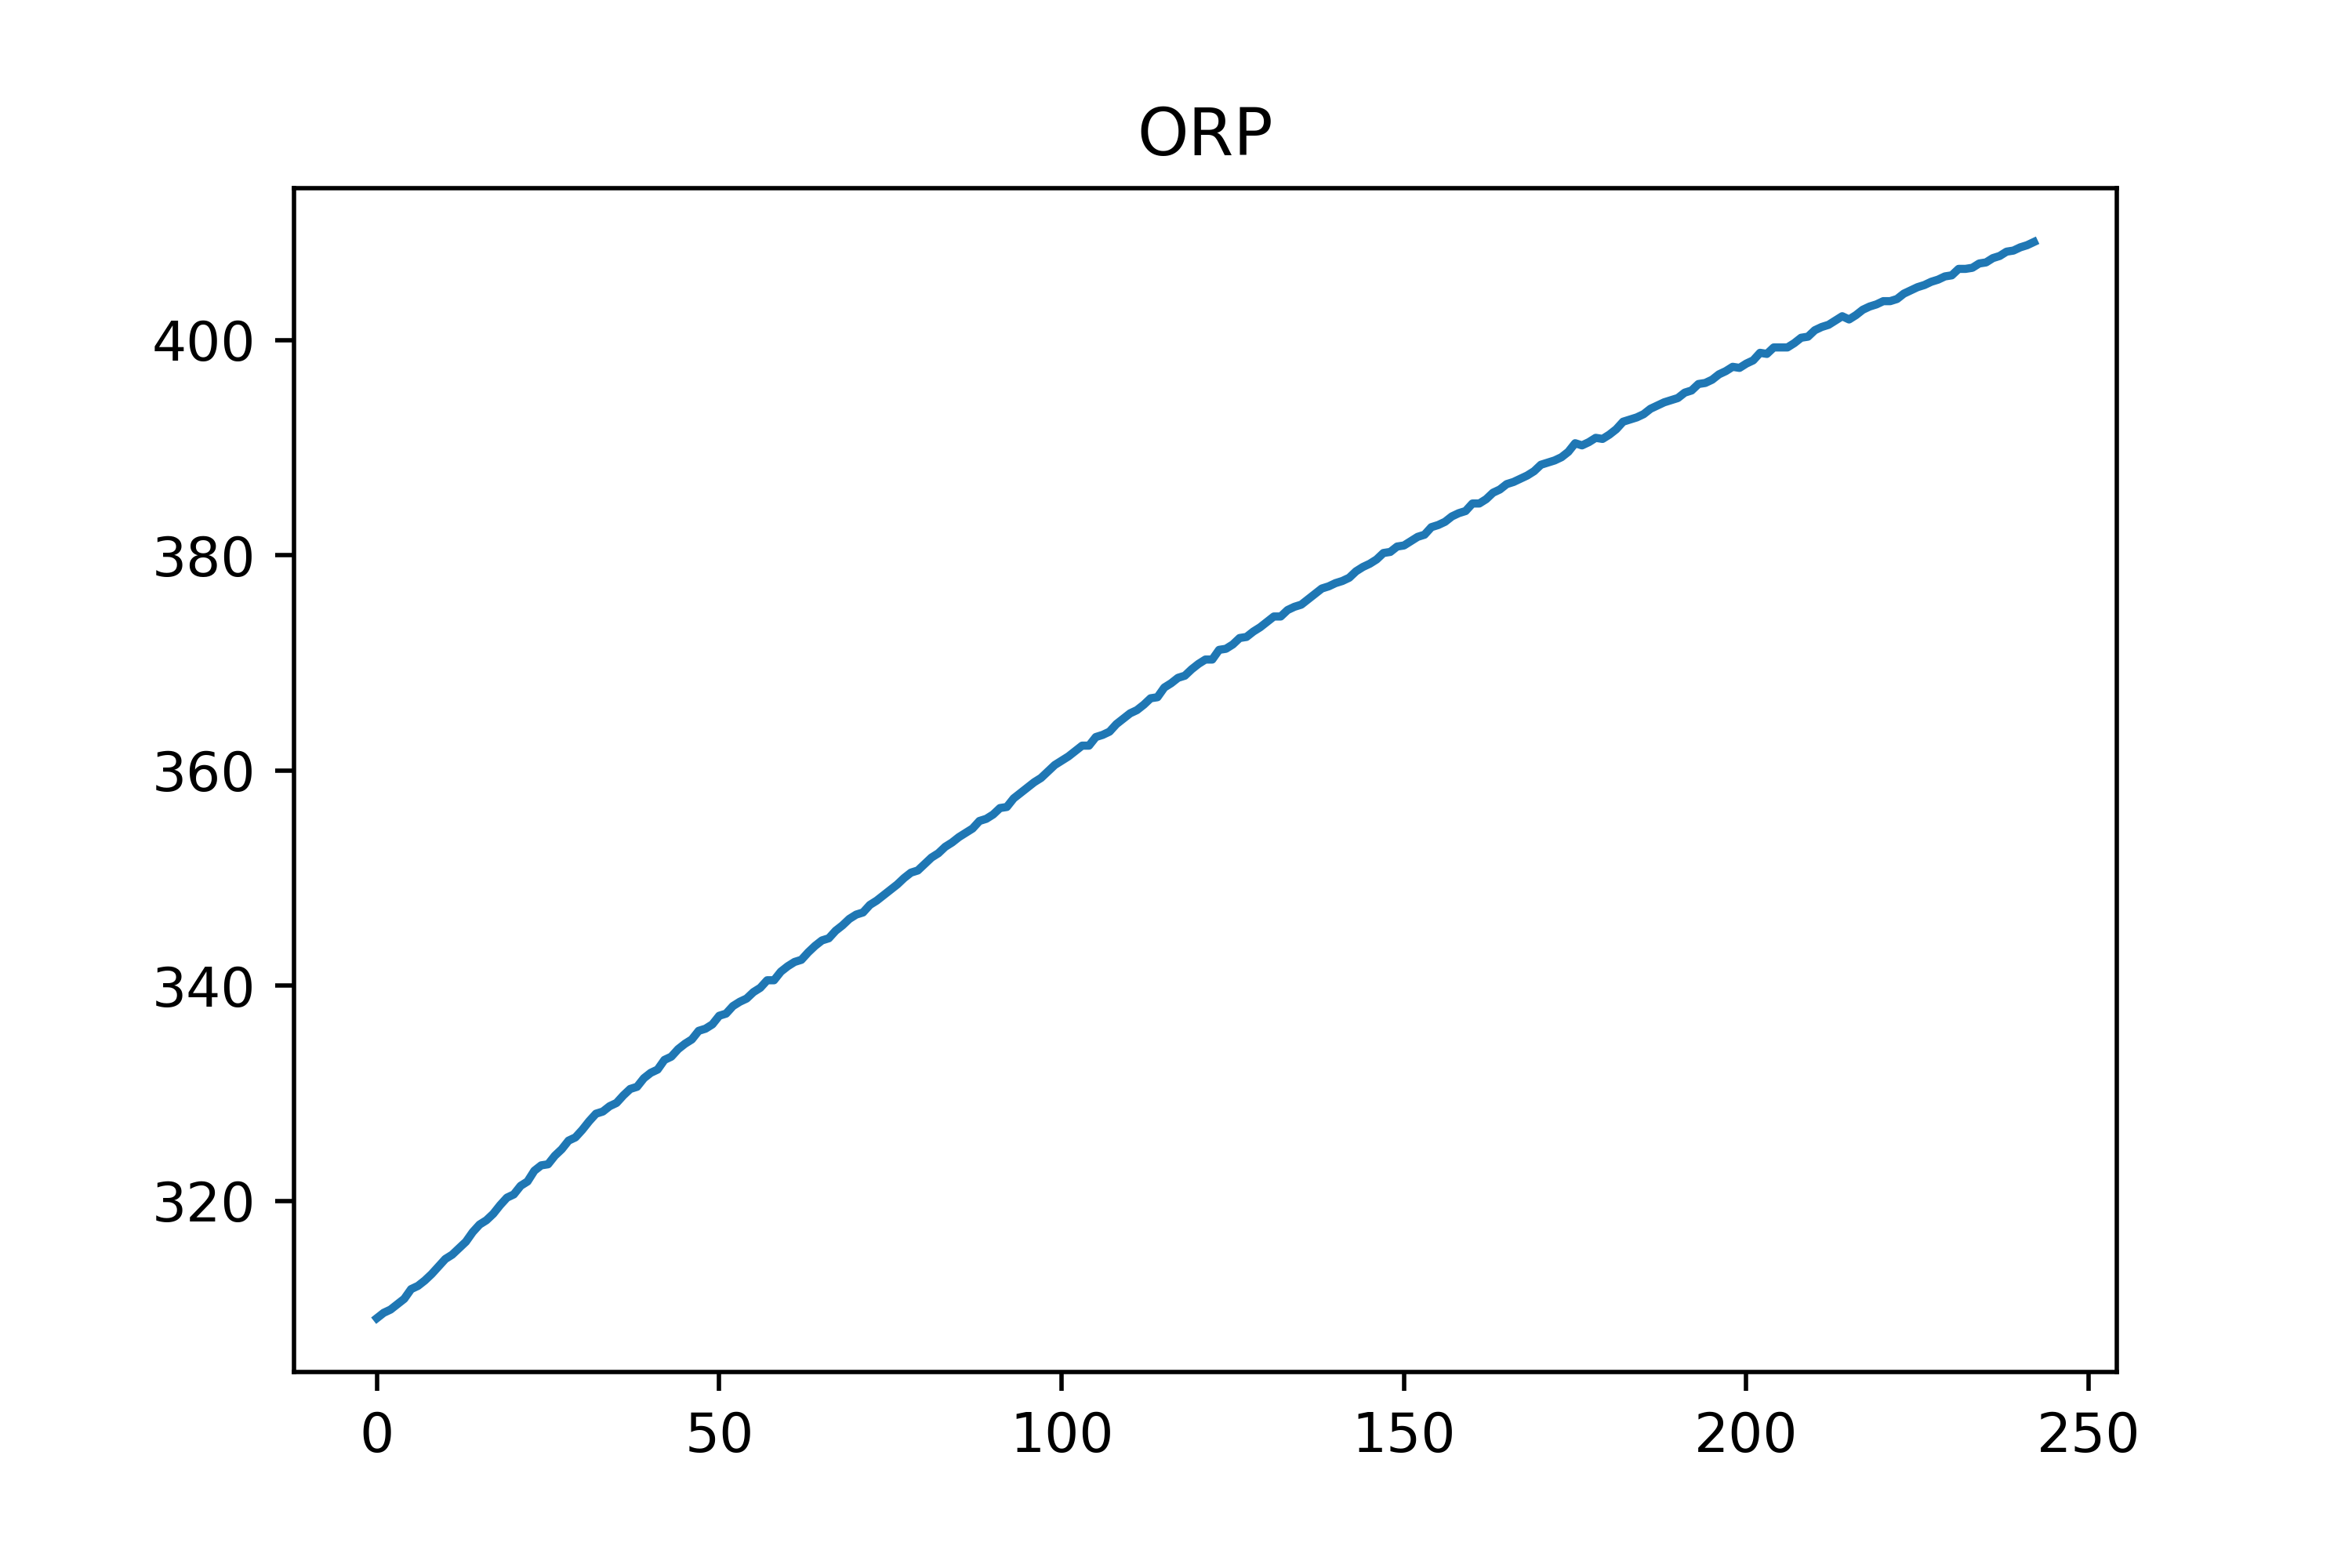
\includegraphics[scale=0.7]{imgss157.png}
	\caption{ORP en tanque de mezclado a las 10 de la mañana.}
	\label{fig:figura1000_4}
\end{figure}

\begin{figure}[h]
	\centering
	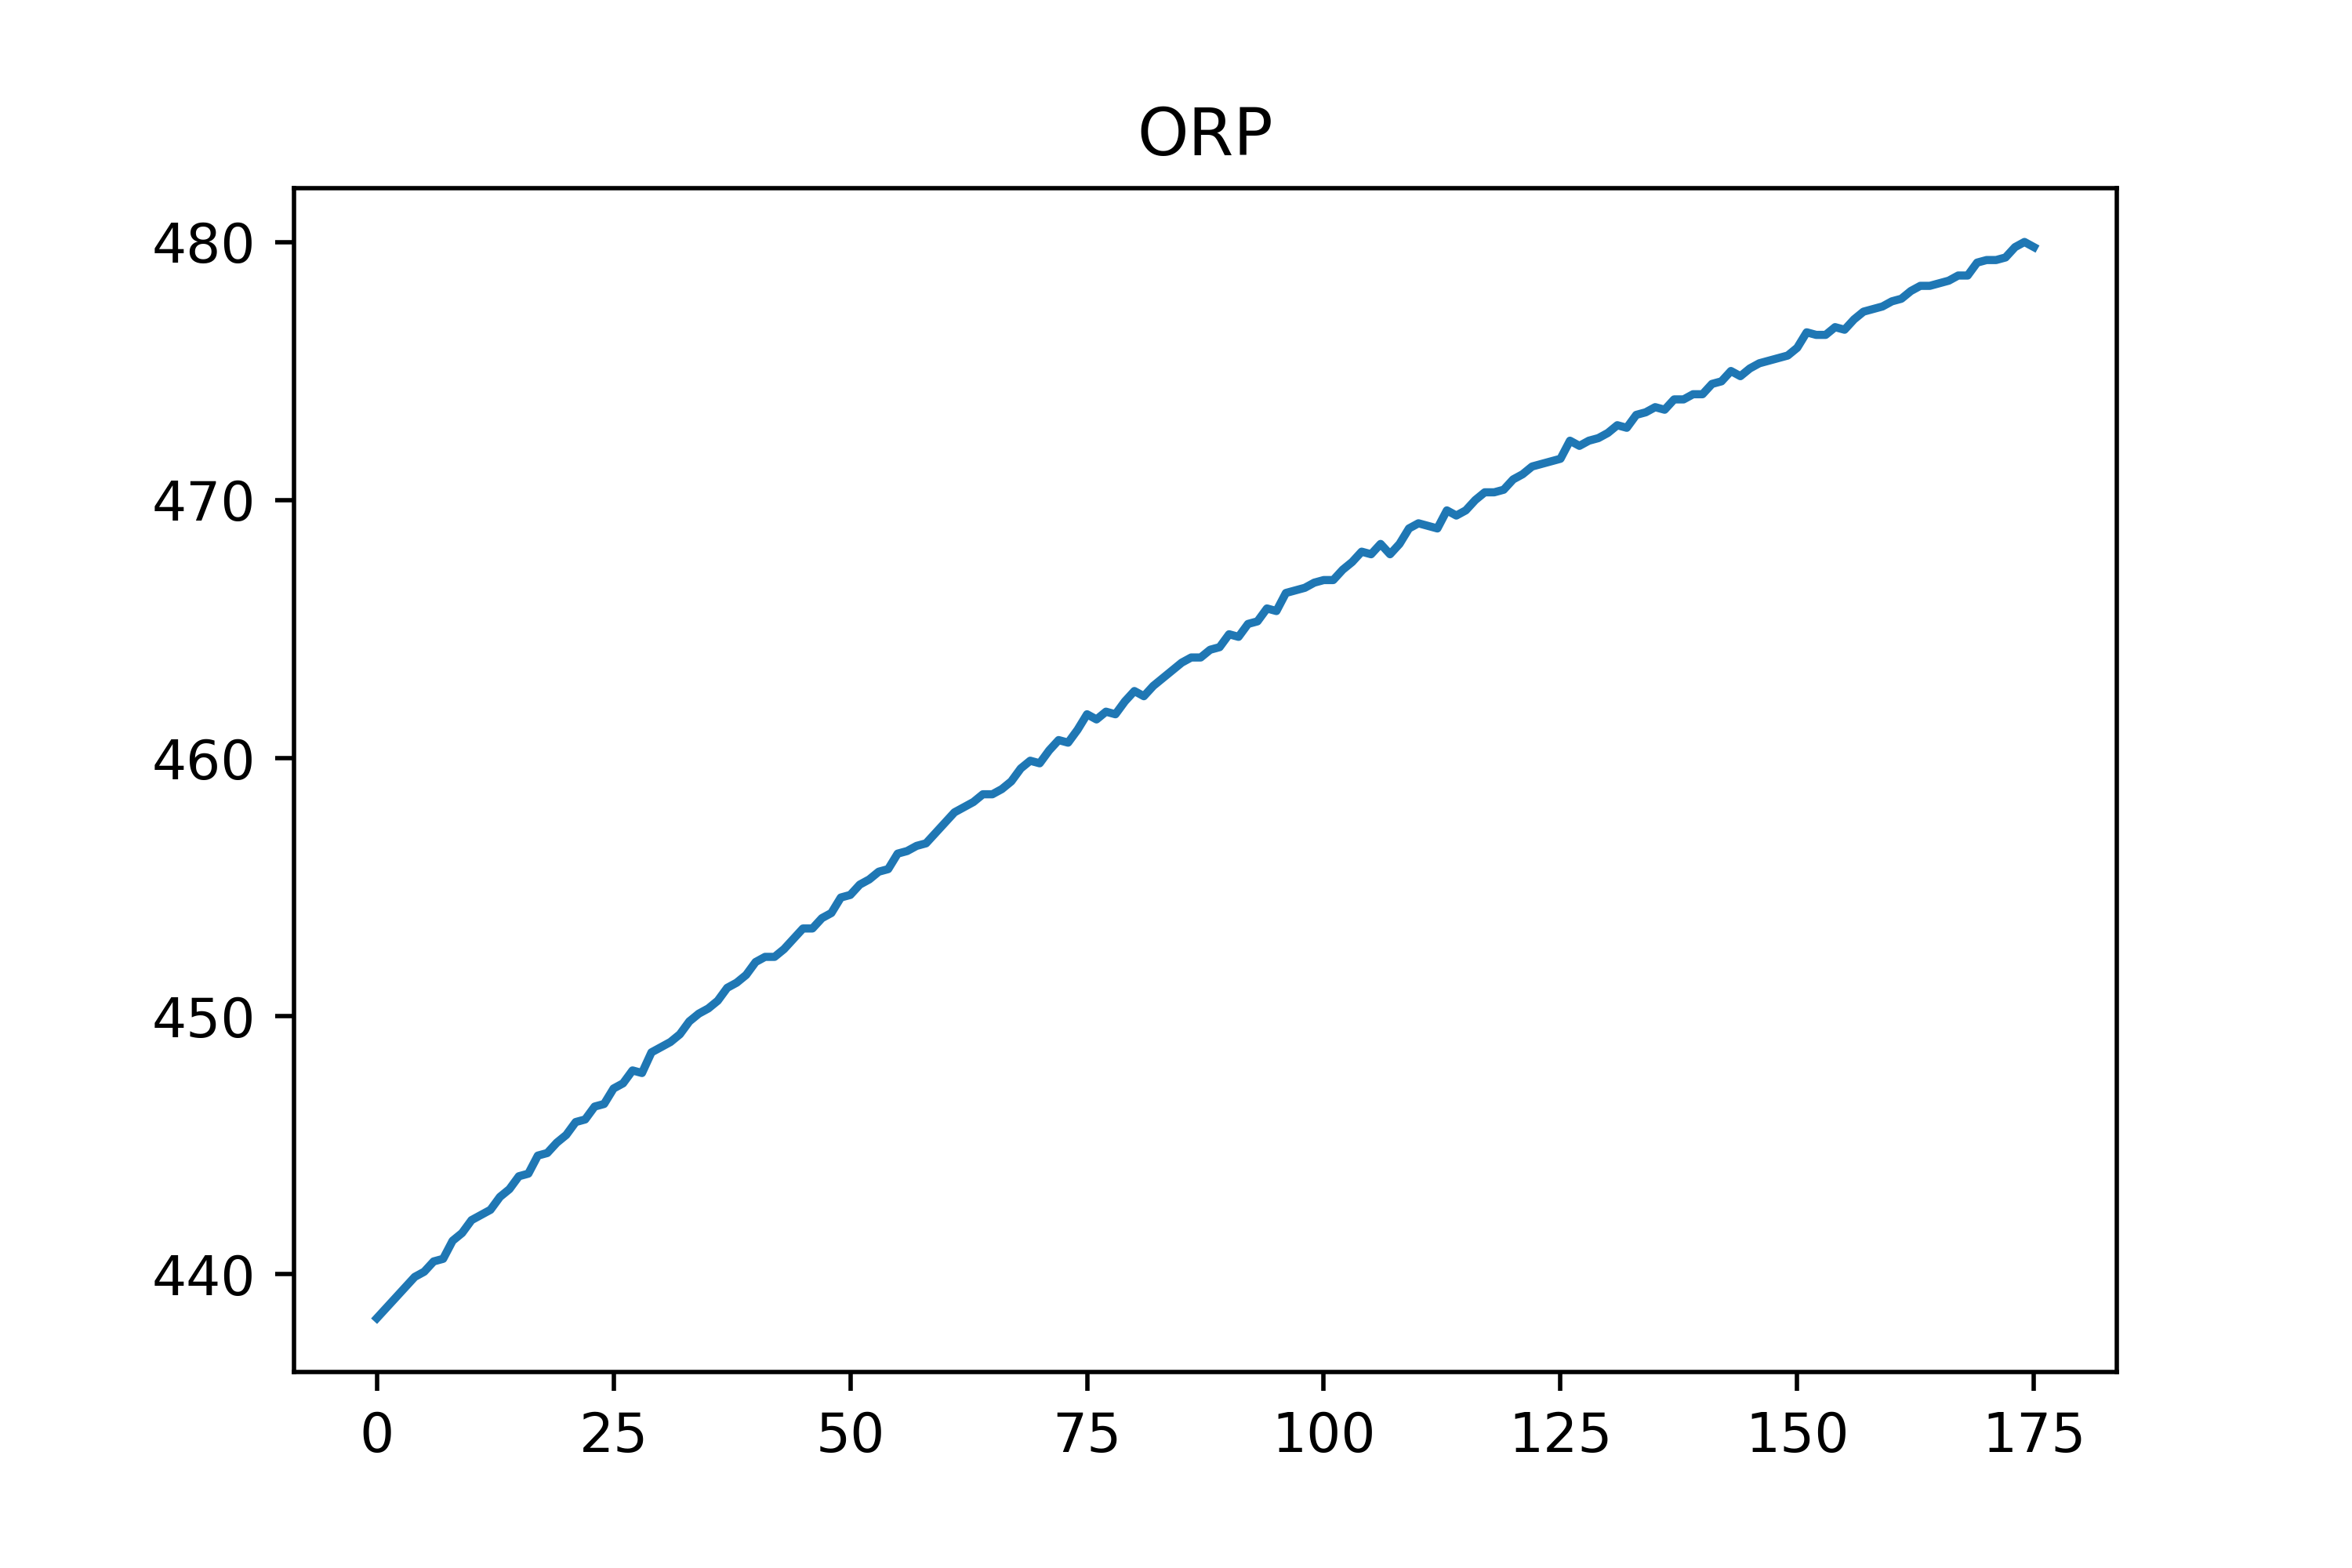
\includegraphics[scale=0.7]{imgss158.png}
	\caption{ORP en tanque de mezclado a las 12 de la tarde.}
	\label{fig:figura1000_5}
\end{figure}

\clearpage

\begin{figure}[h]
	\centering
	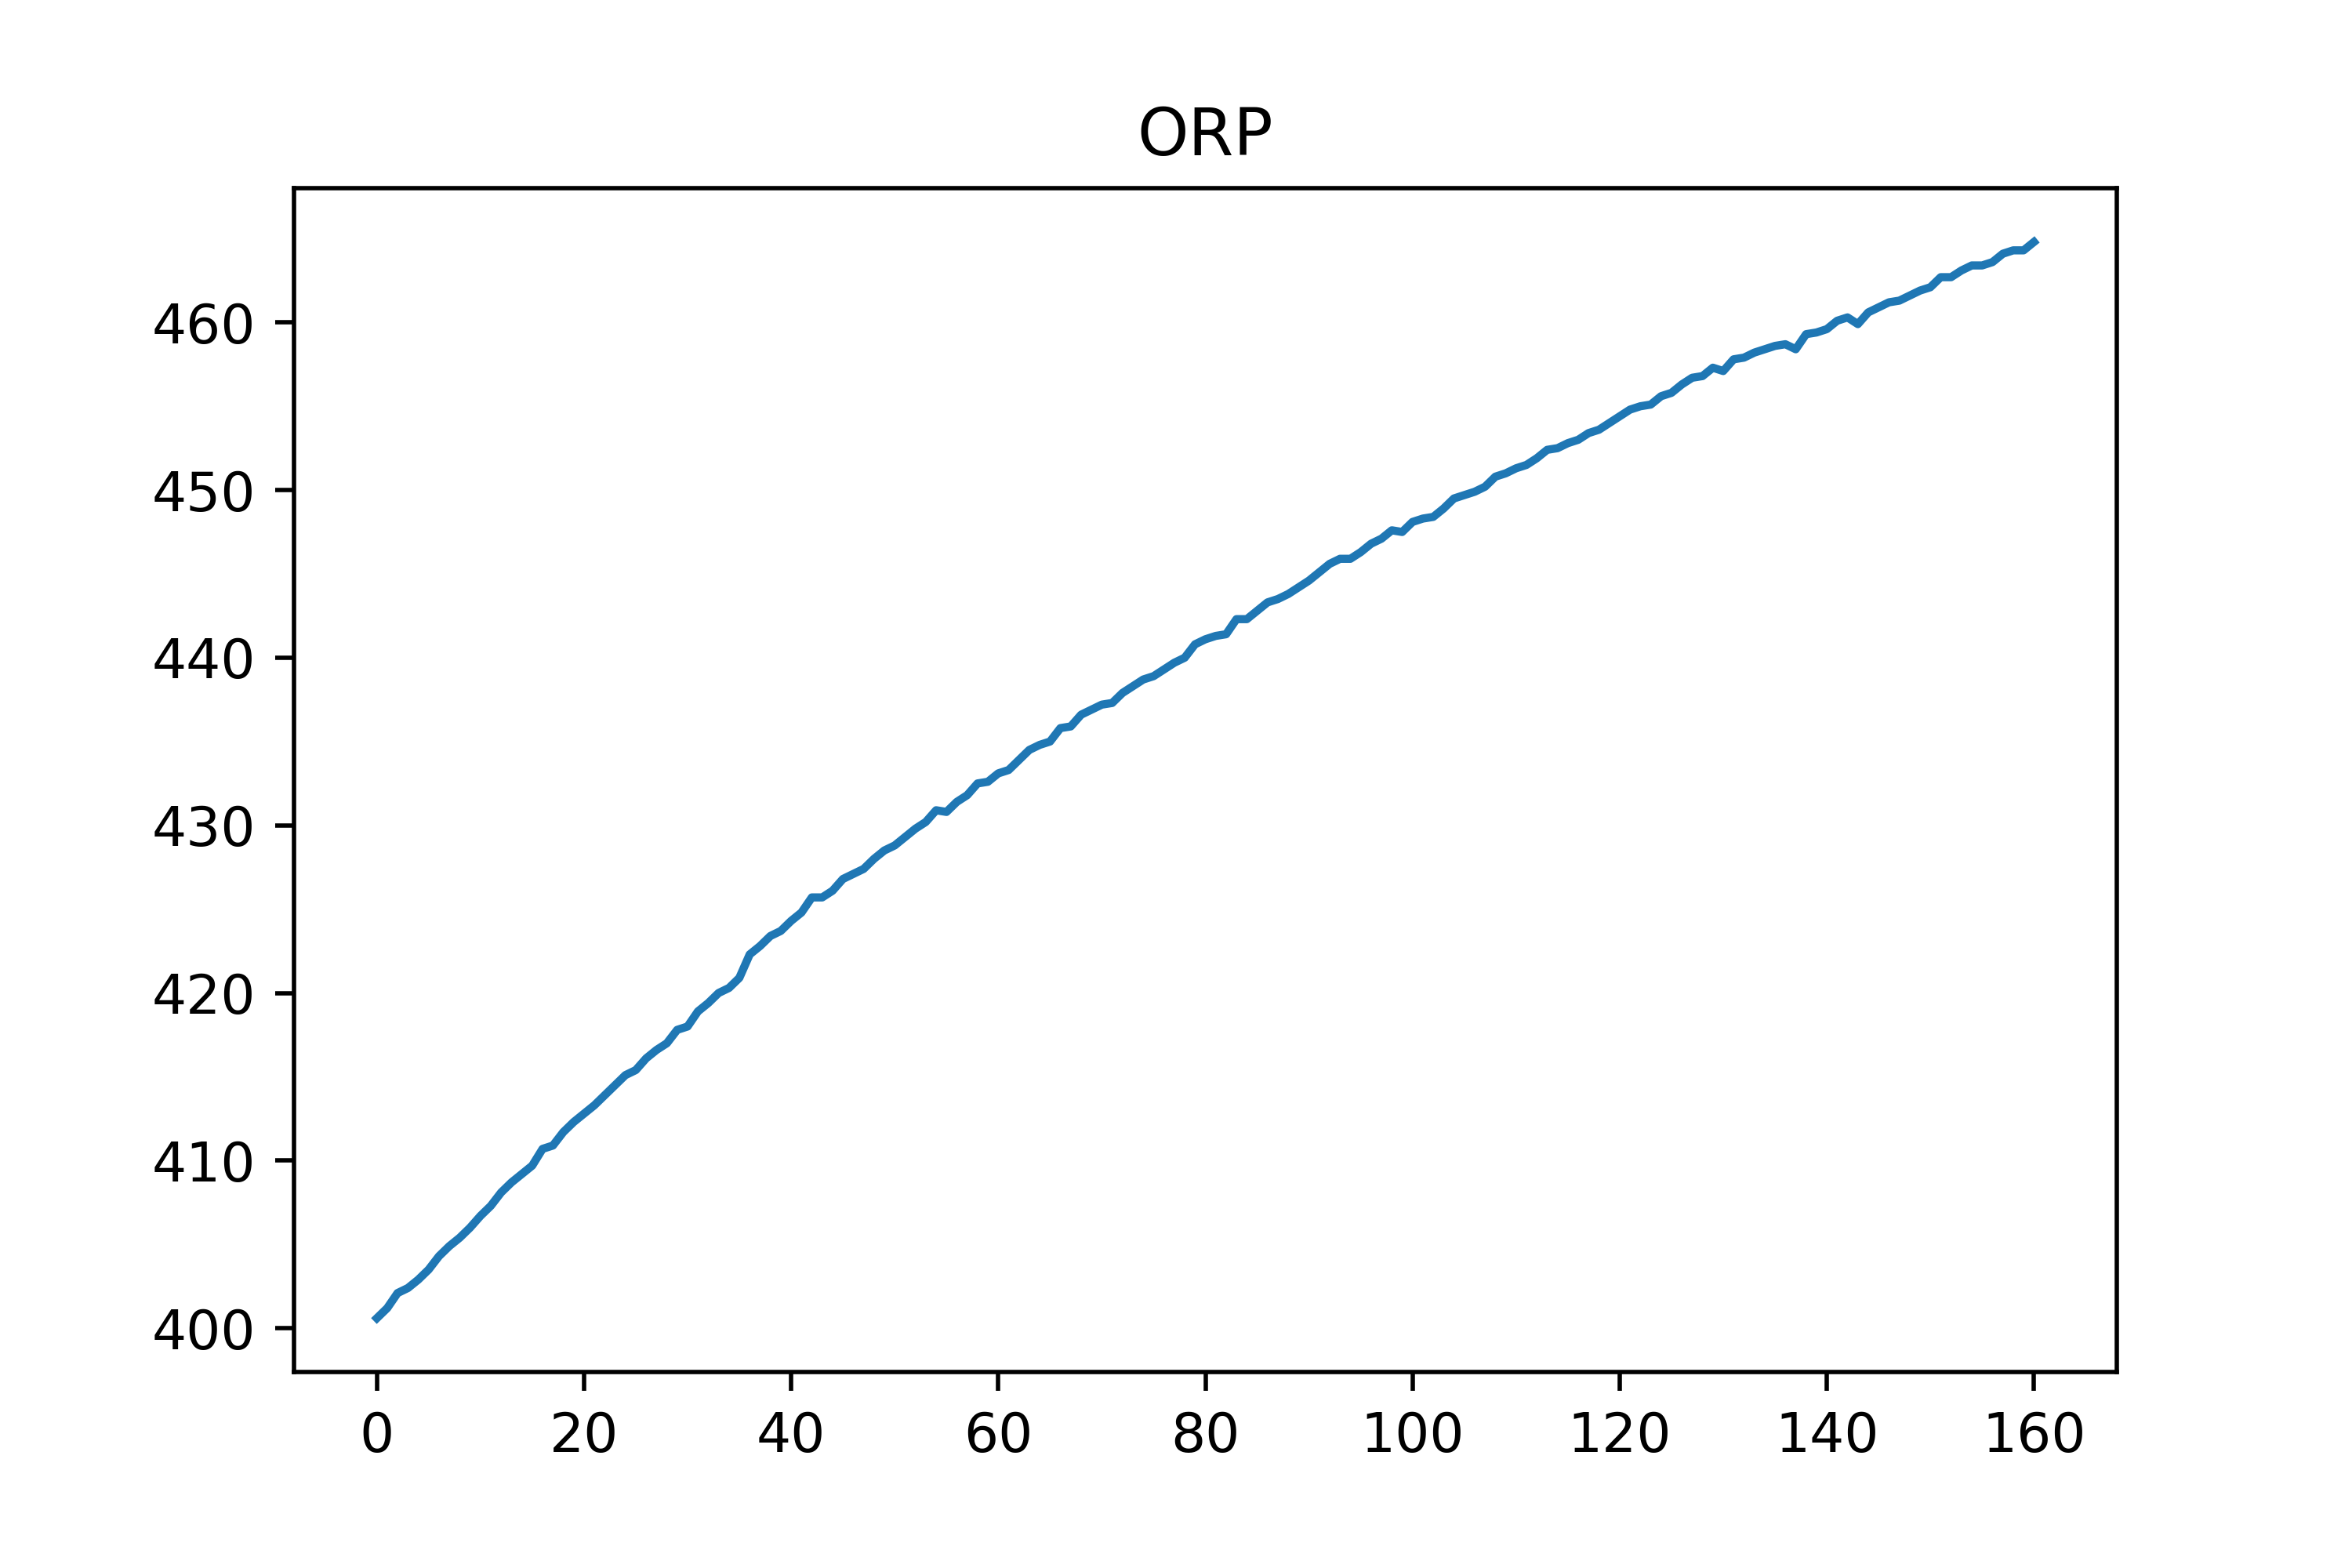
\includegraphics[scale=0.7]{imgss159.png}
	\caption{ORP en tanque de mezclado a las 2 de la tarde.}
	\label{fig:figura1000_6}
\end{figure}

\begin{figure}[h]
	\centering
	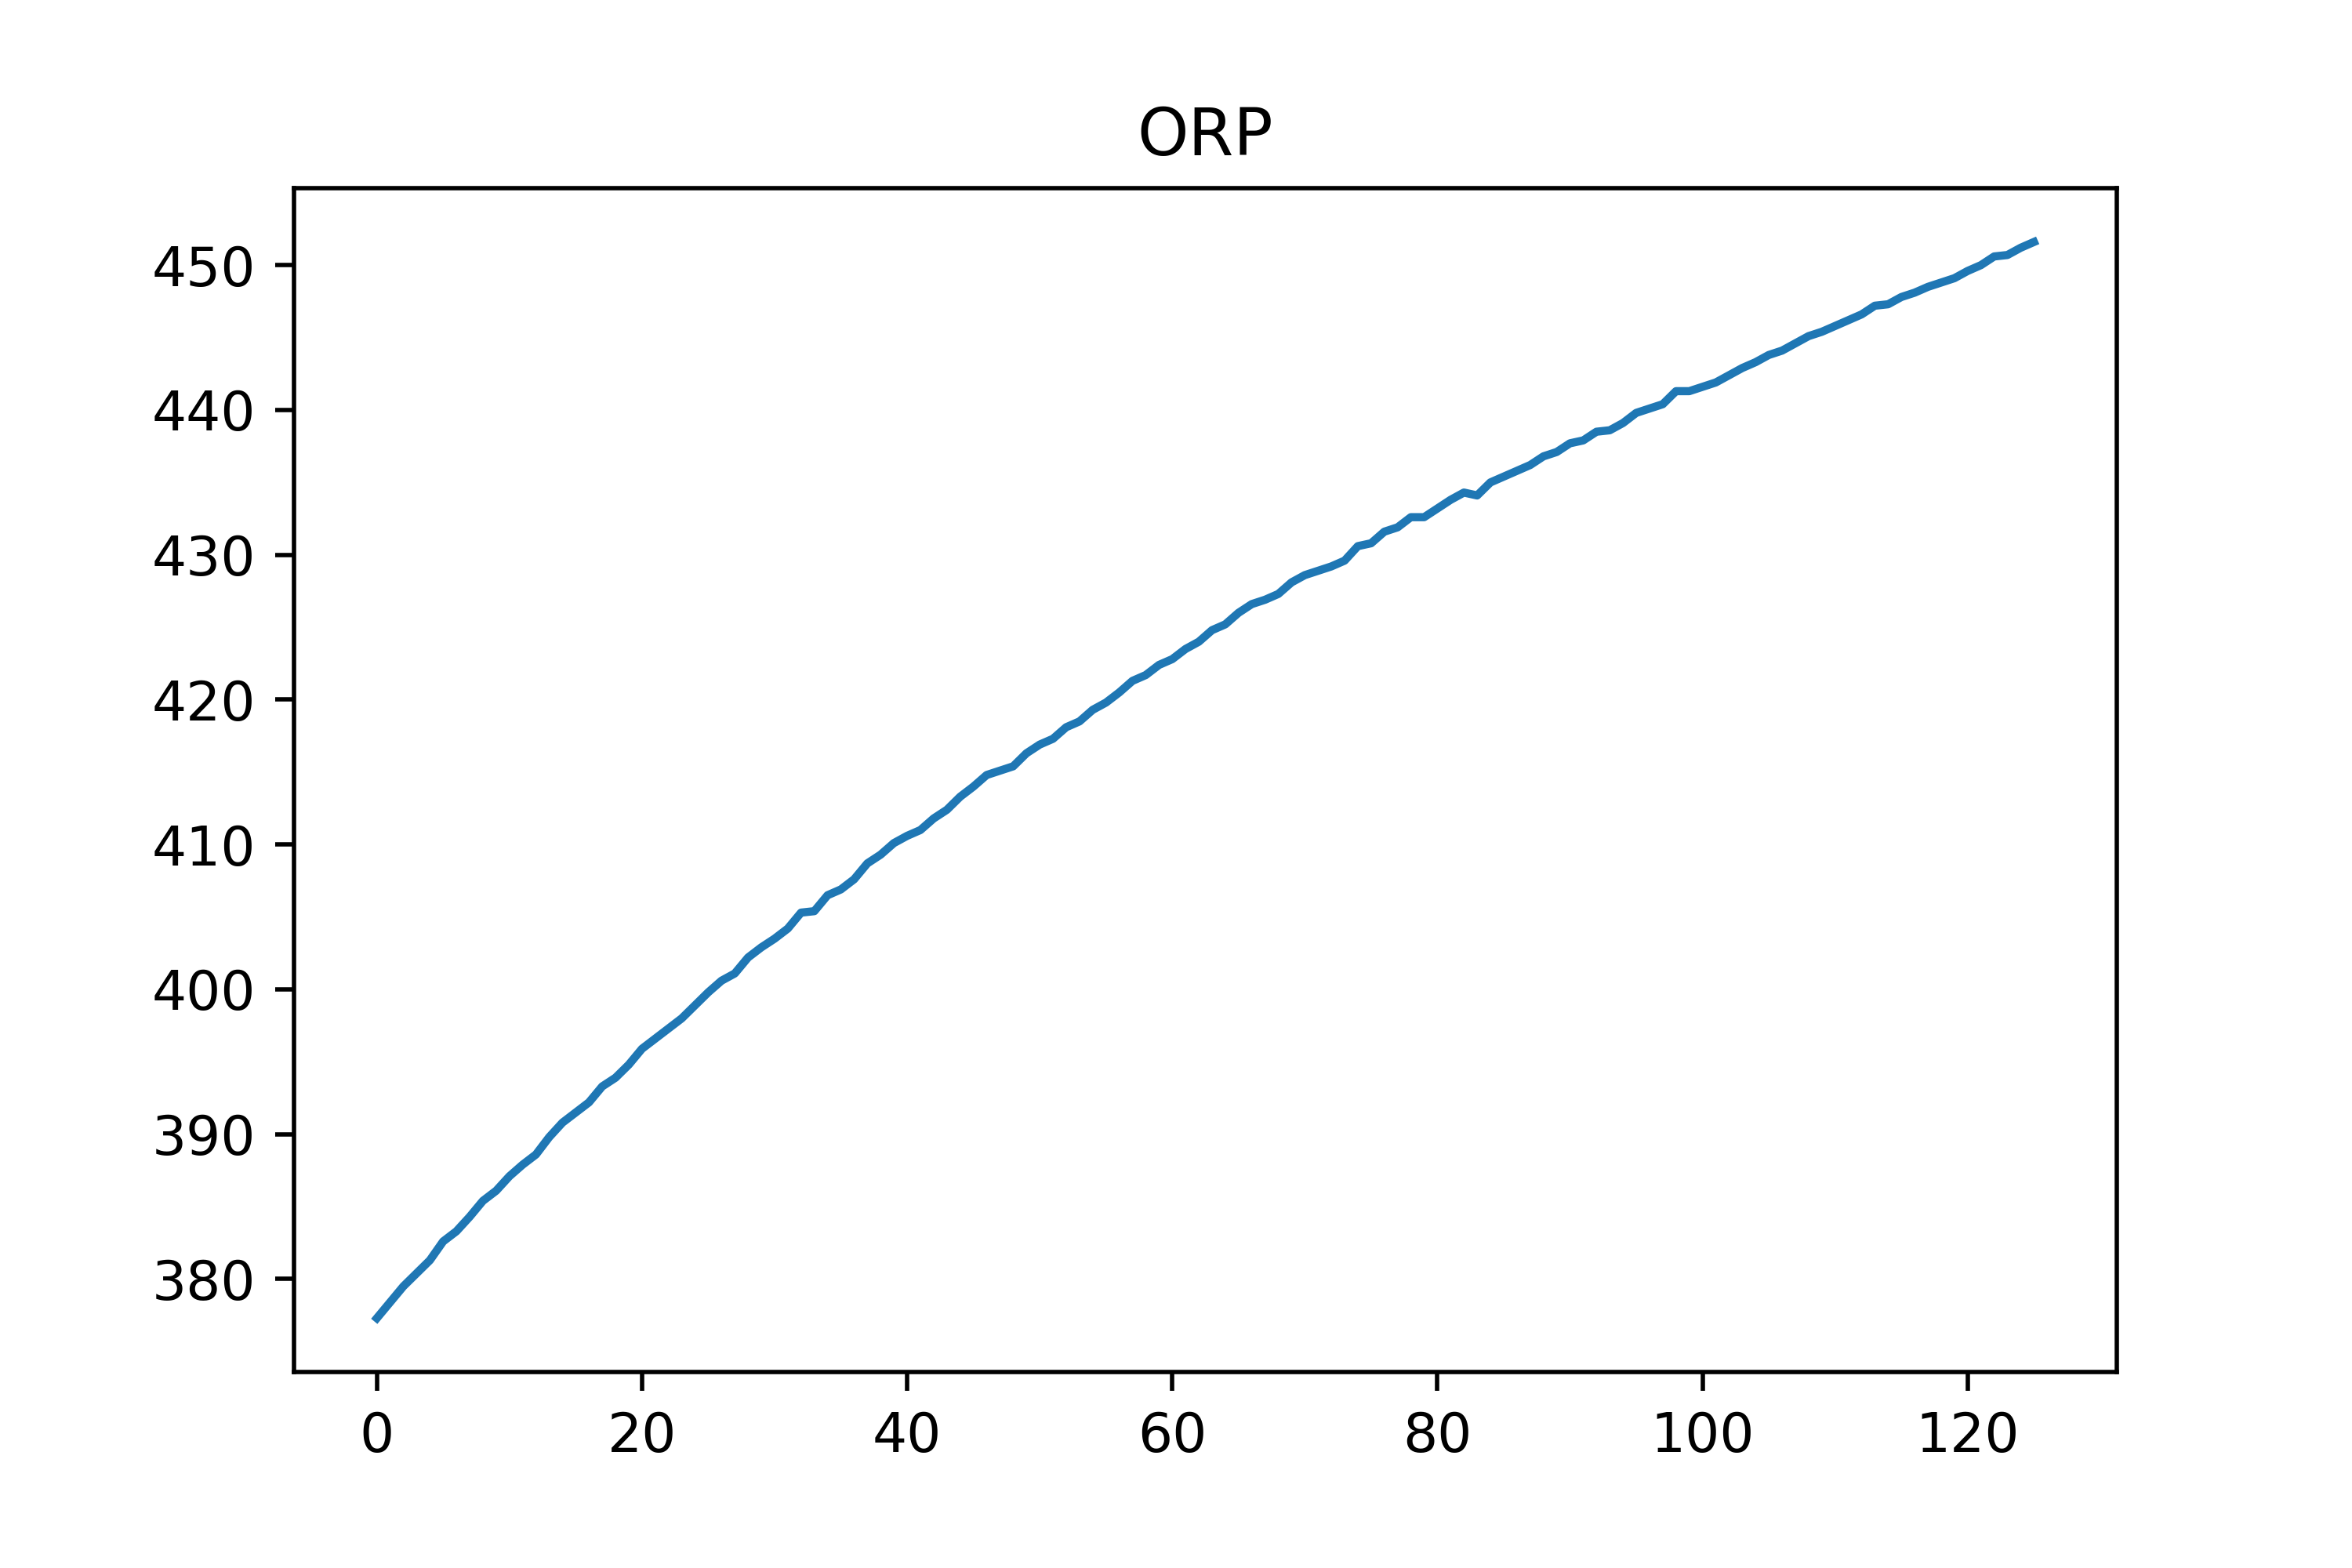
\includegraphics[scale=0.7]{imgss160.png}
	\caption{ORP en tanque de mezclado a las 4 de la tarde.}
	\label{fig:figura1000_7}
\end{figure}

Para la etapa de agua potable, se muestran las siguientes mediciones en los diferentes horarios en la \autoref{fig:figura1000_8}, \autoref{fig:figura1000_9}, \autoref{fig:figura1000_10} y \autoref{fig:figura1000_11}. 
En los ejes horizontales se tiene el número de muestras y la magnitud de la variable se encuentra en el eje vertical de las gráficas.

\clearpage

\begin{figure}[h]
	\centering
	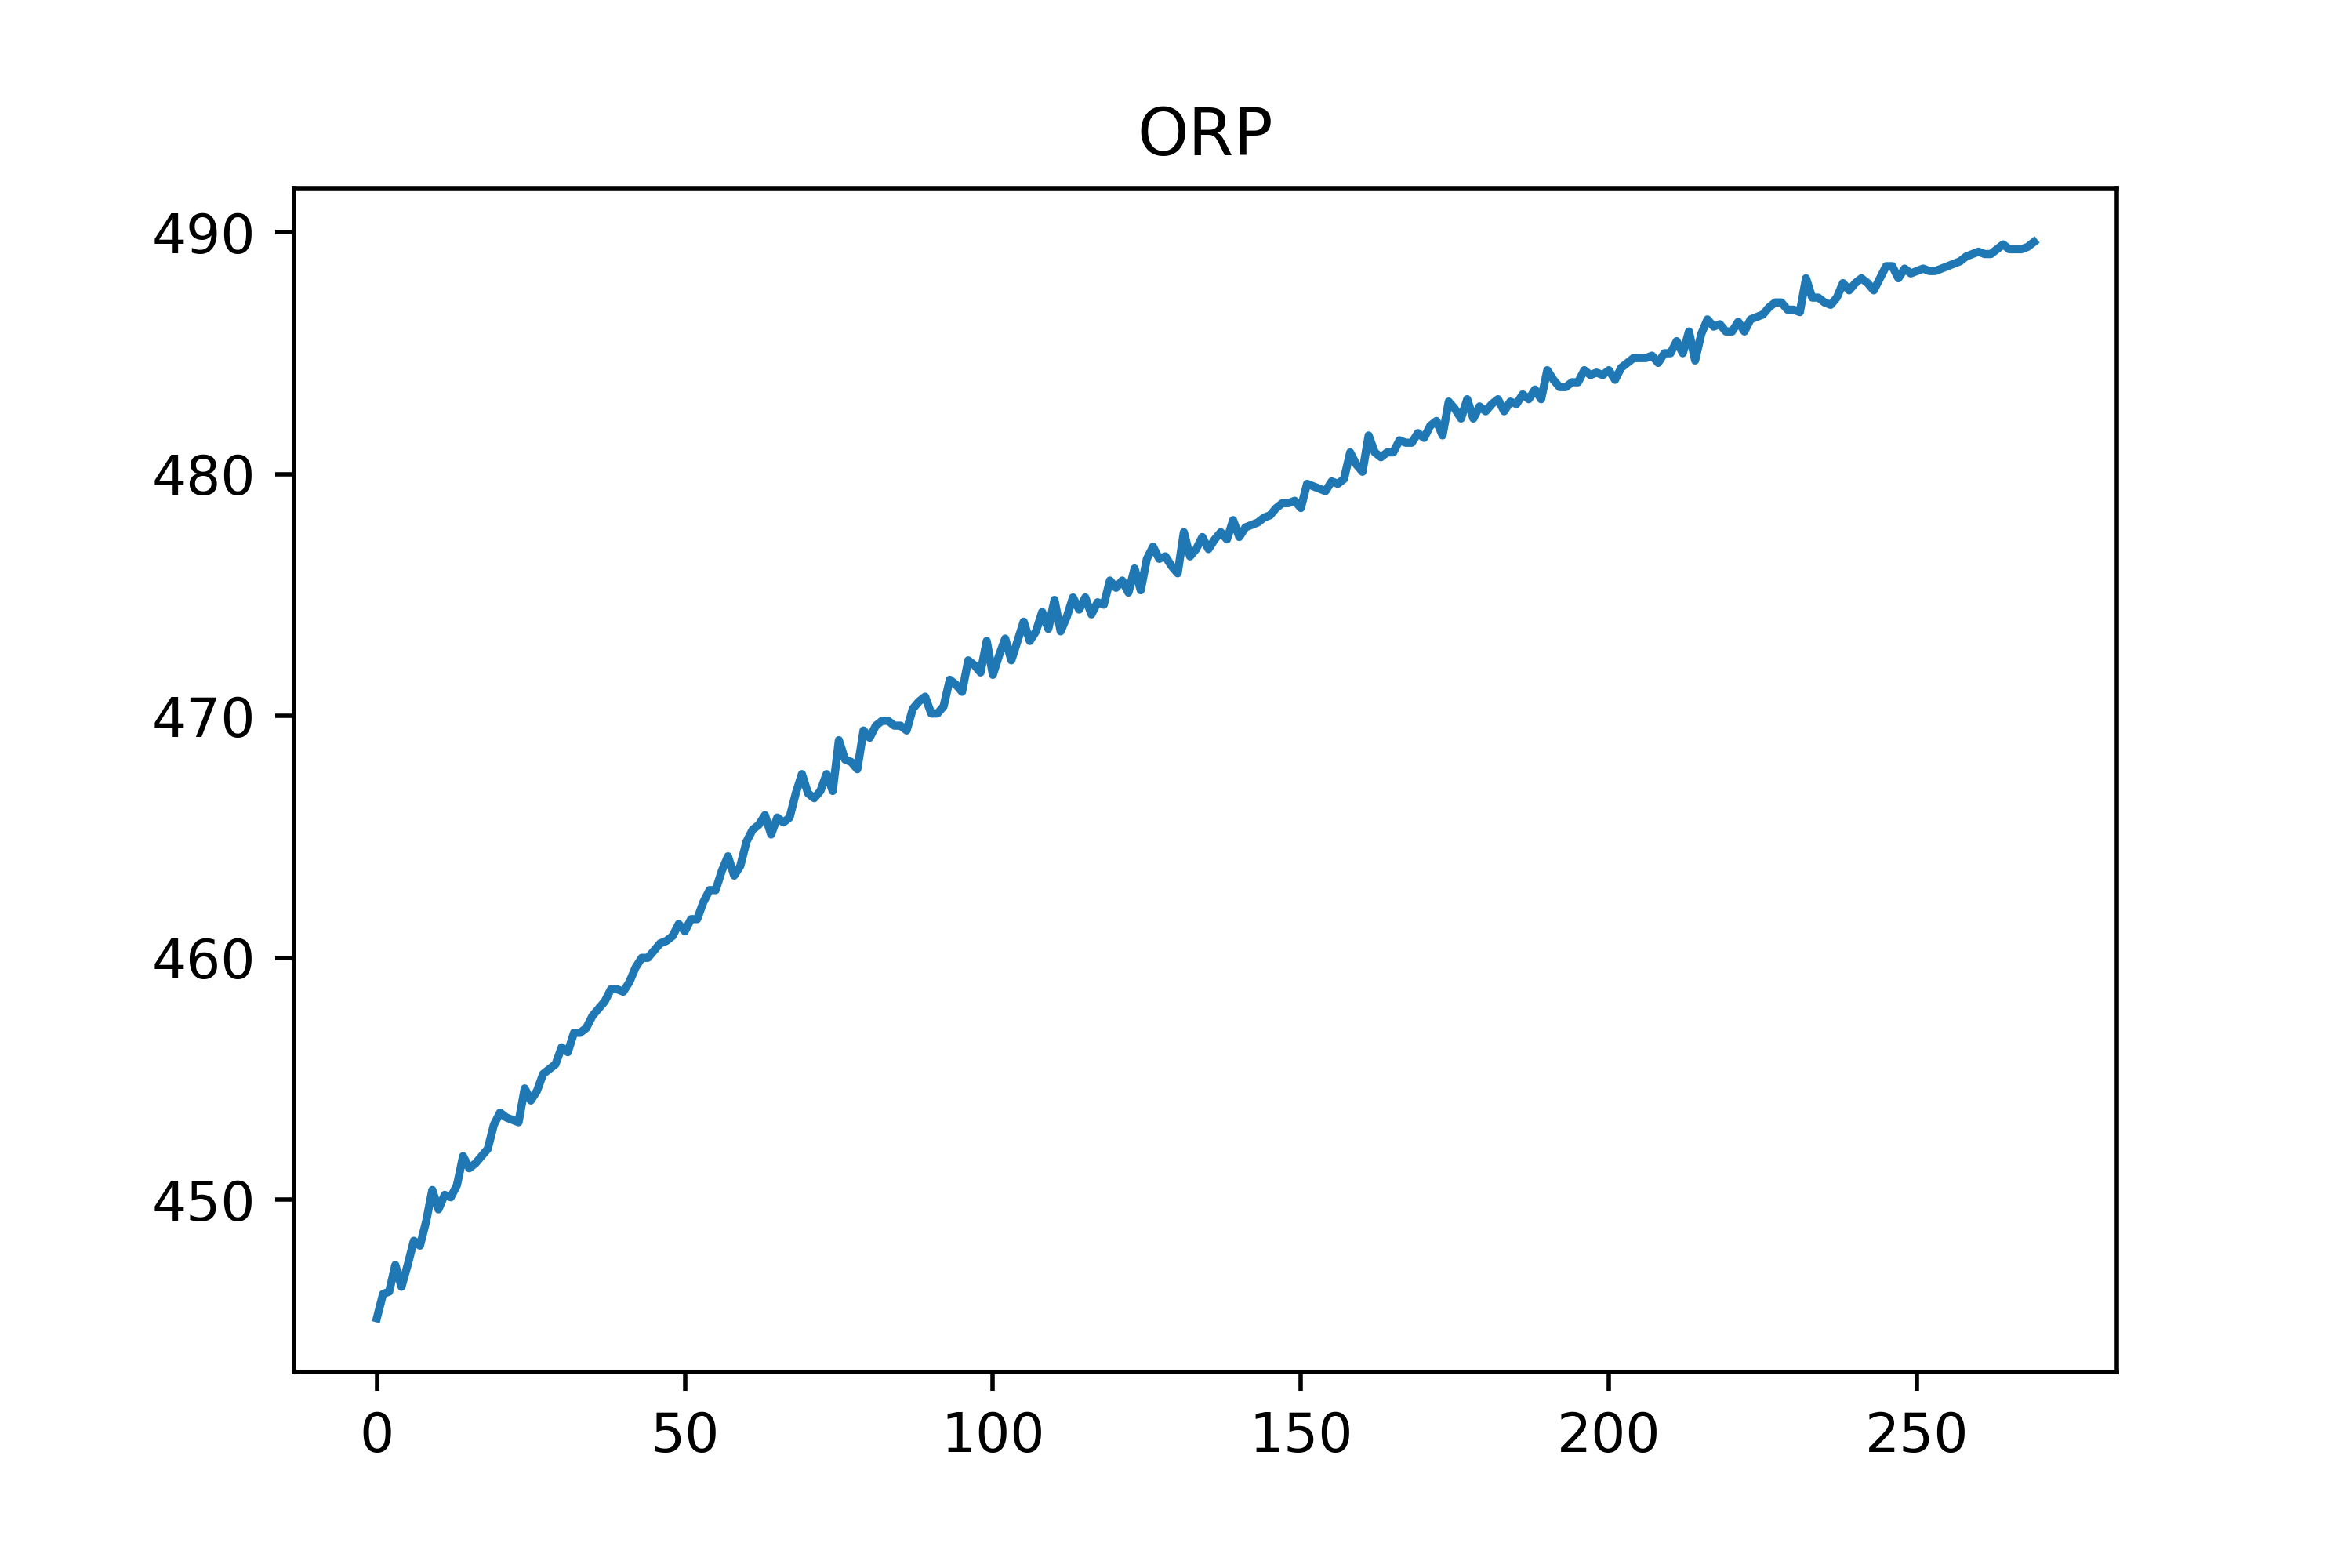
\includegraphics[scale=0.7]{imgss161.png}
	\caption{ORP en agua potable a las 10 de la mañana.}
	\label{fig:figura1000_8}
\end{figure}

\begin{figure}[h]
	\centering
	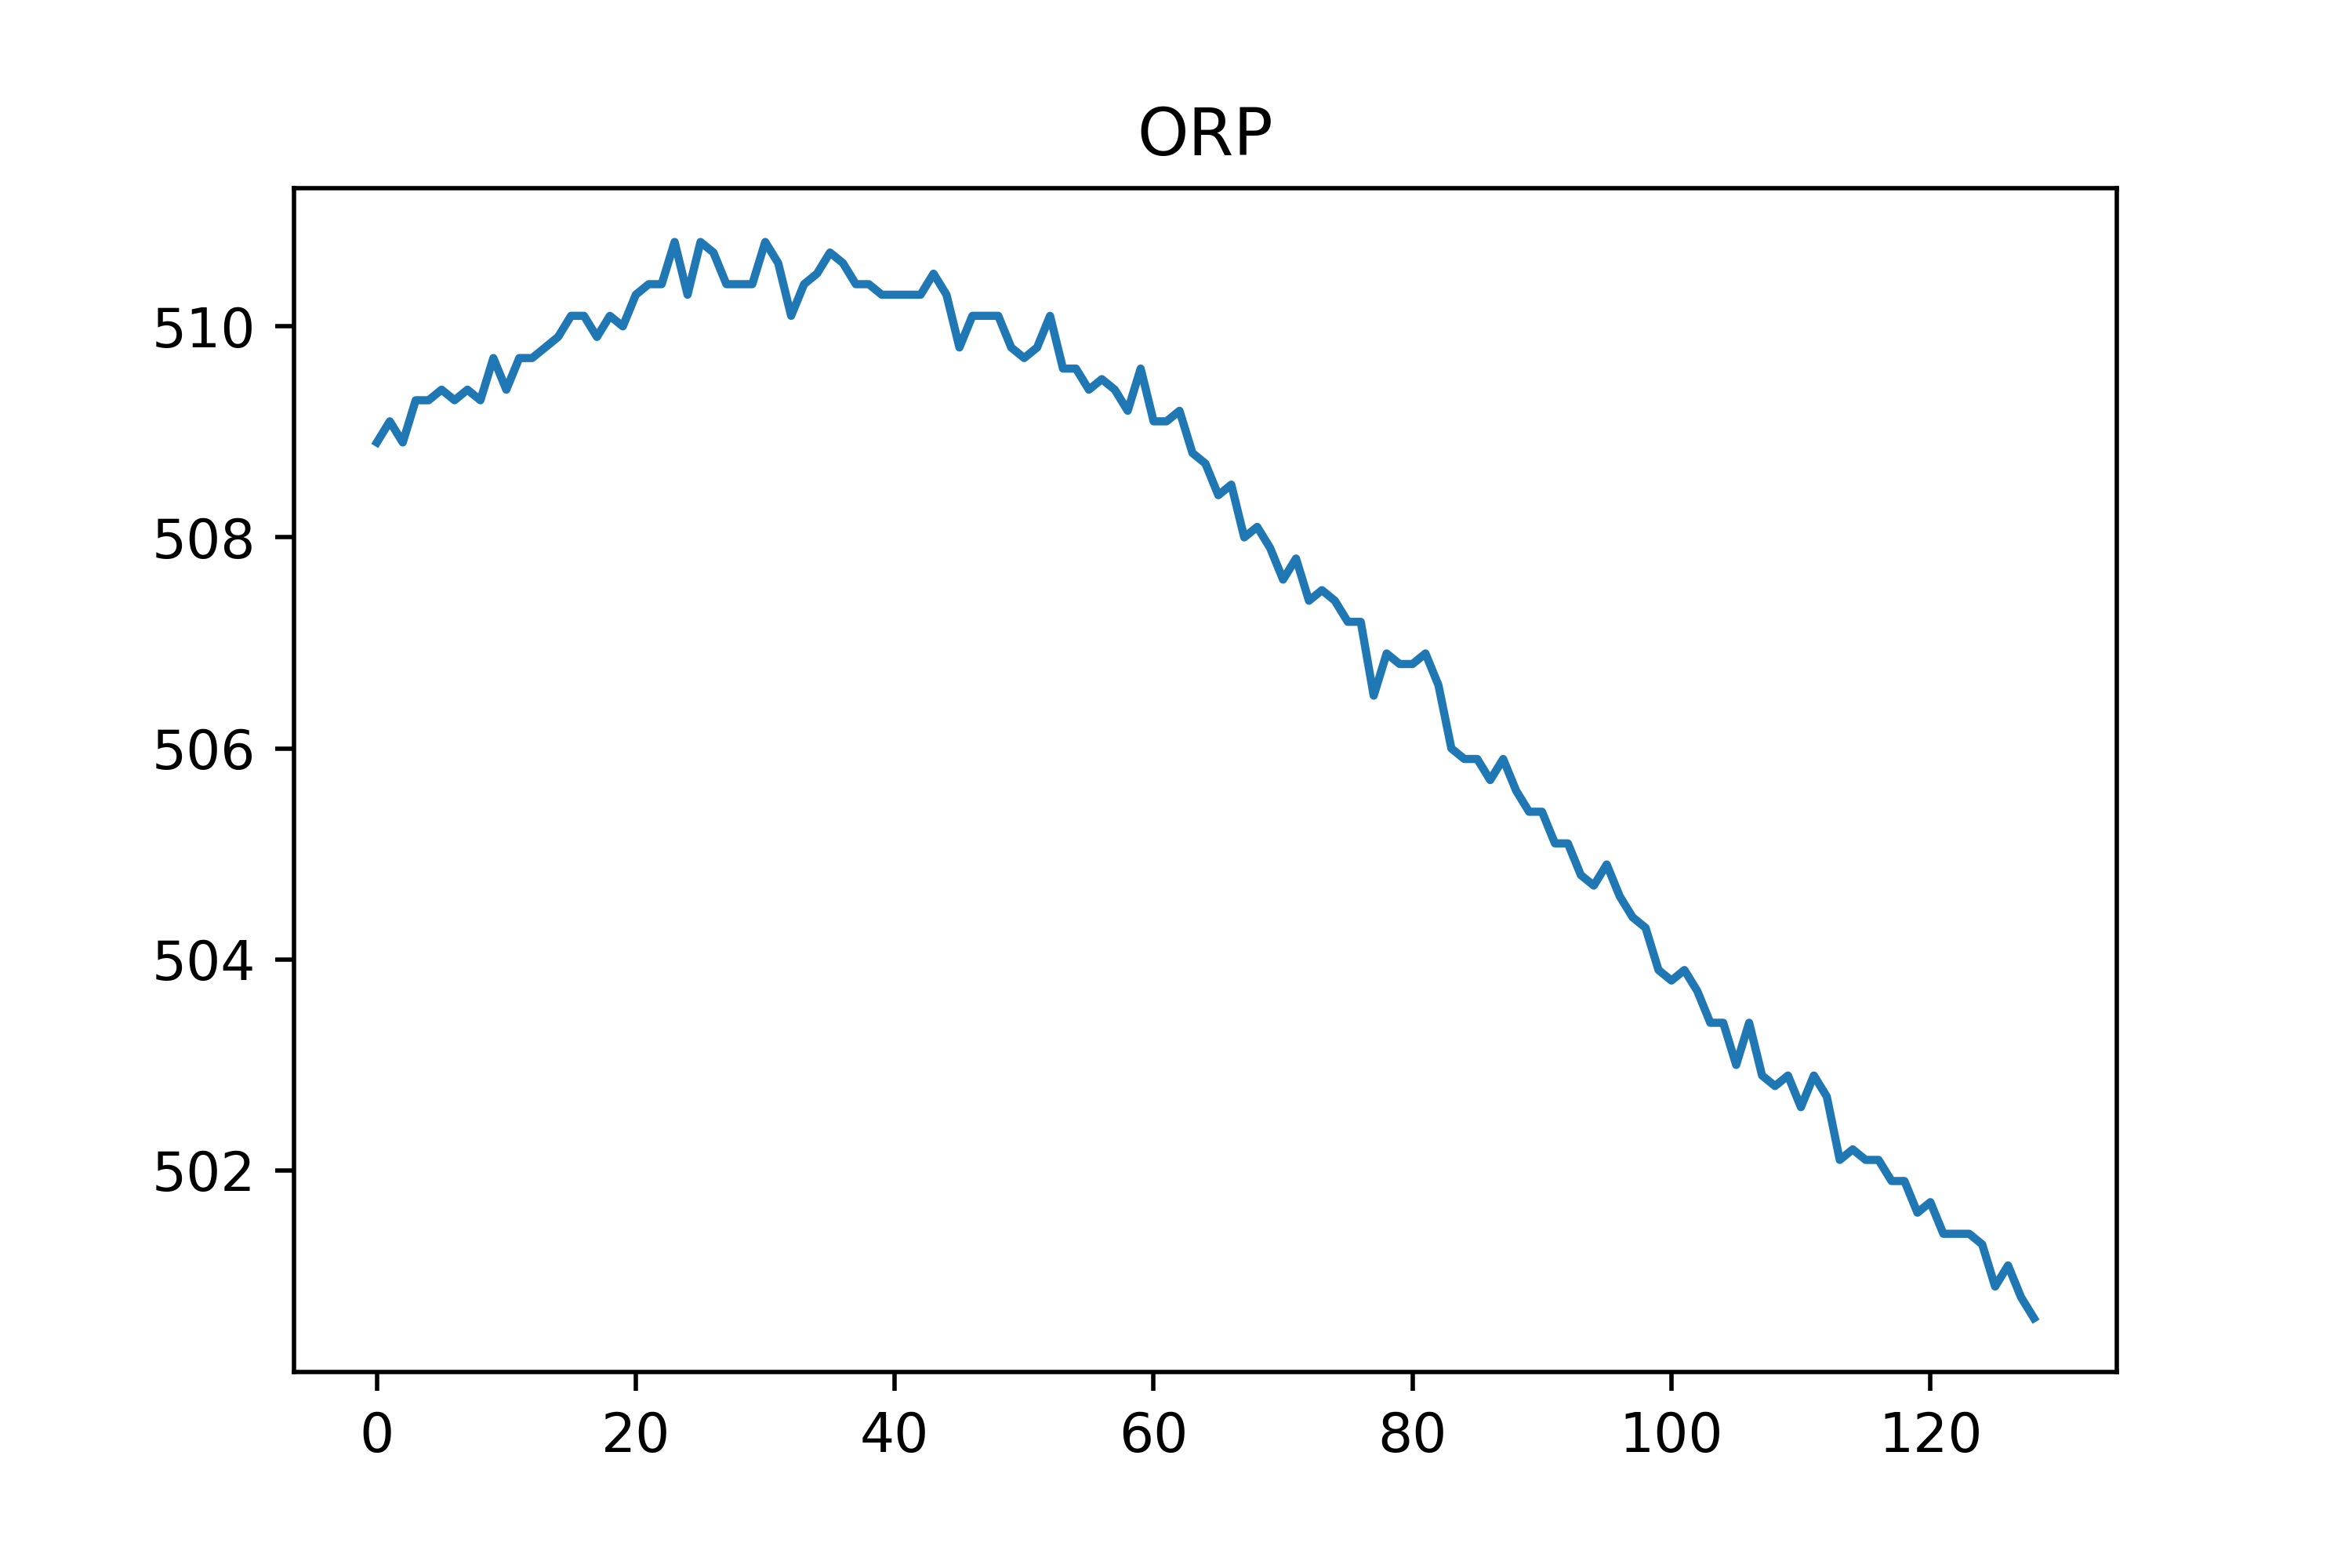
\includegraphics[scale=0.7]{imgss162.png}
	\caption{ORP en agua potable a las 12 de la tarde.}
	\label{fig:figura1000_9}
\end{figure}

\clearpage

\begin{figure}[h]
	\centering
	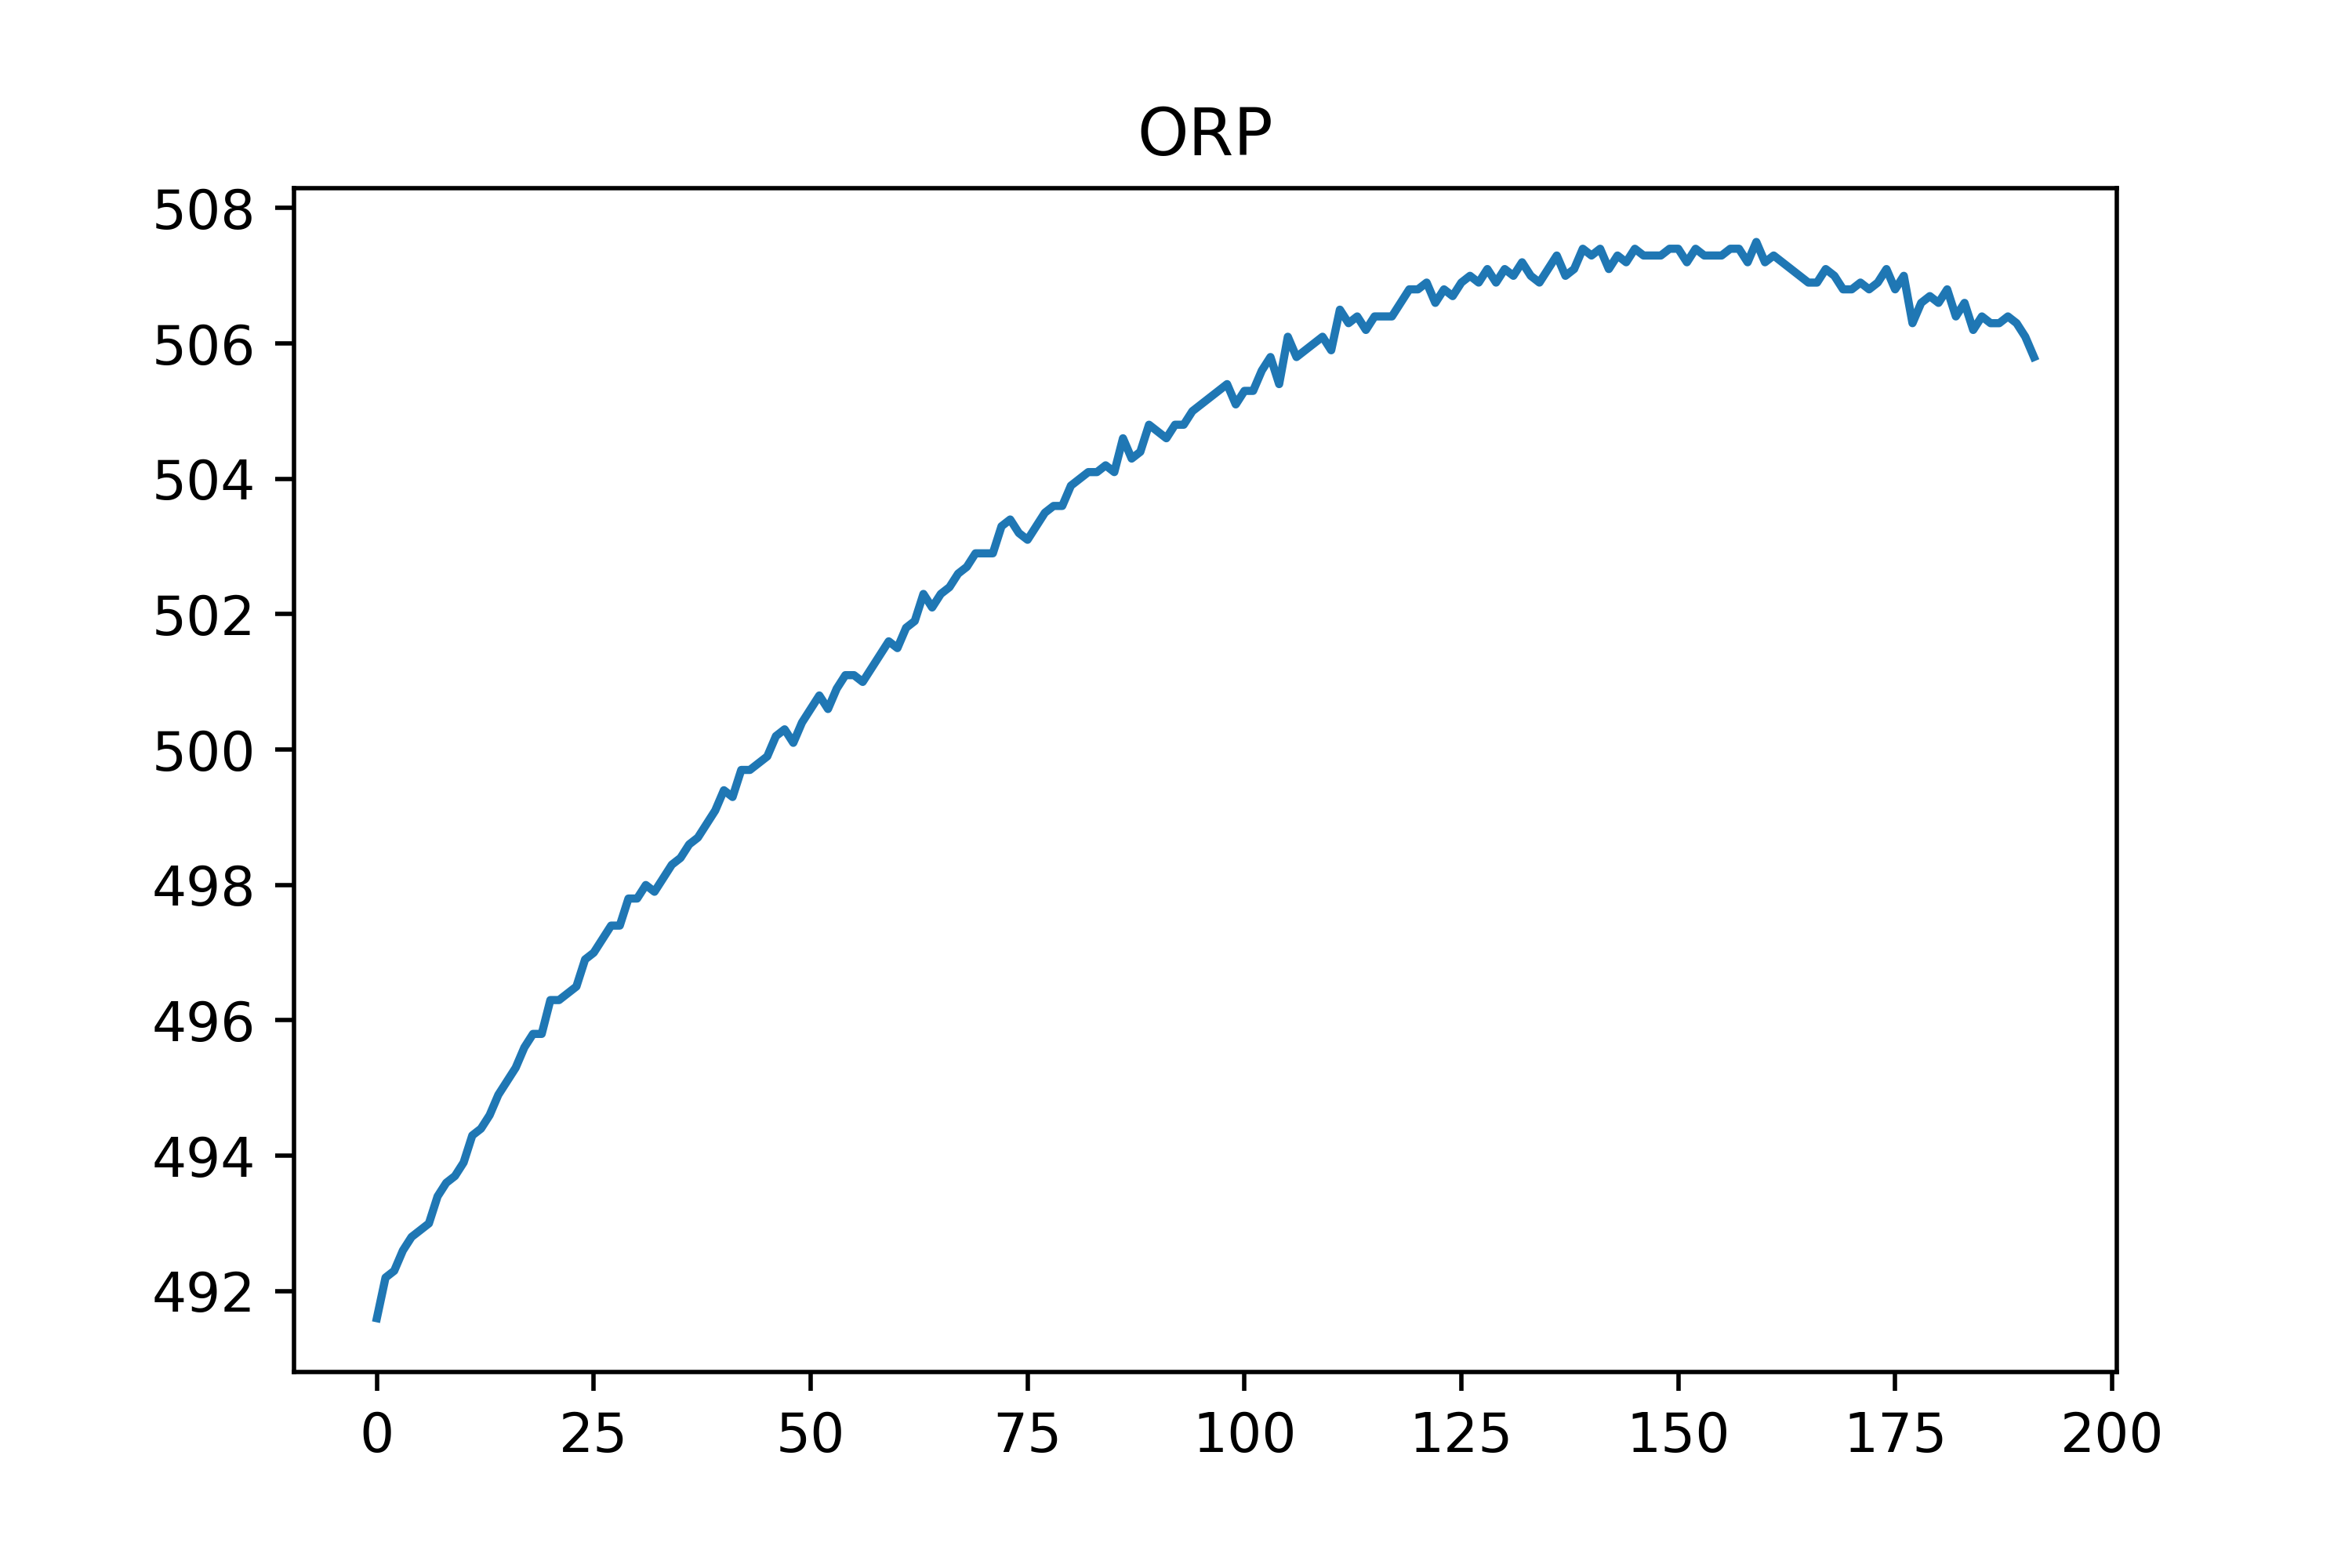
\includegraphics[scale=0.7]{imgss163.png}
	\caption{ORP en agua potable a las 2 de la tarde.}
	\label{fig:figura1000_10}
\end{figure}

\begin{figure}[h]
	\centering
	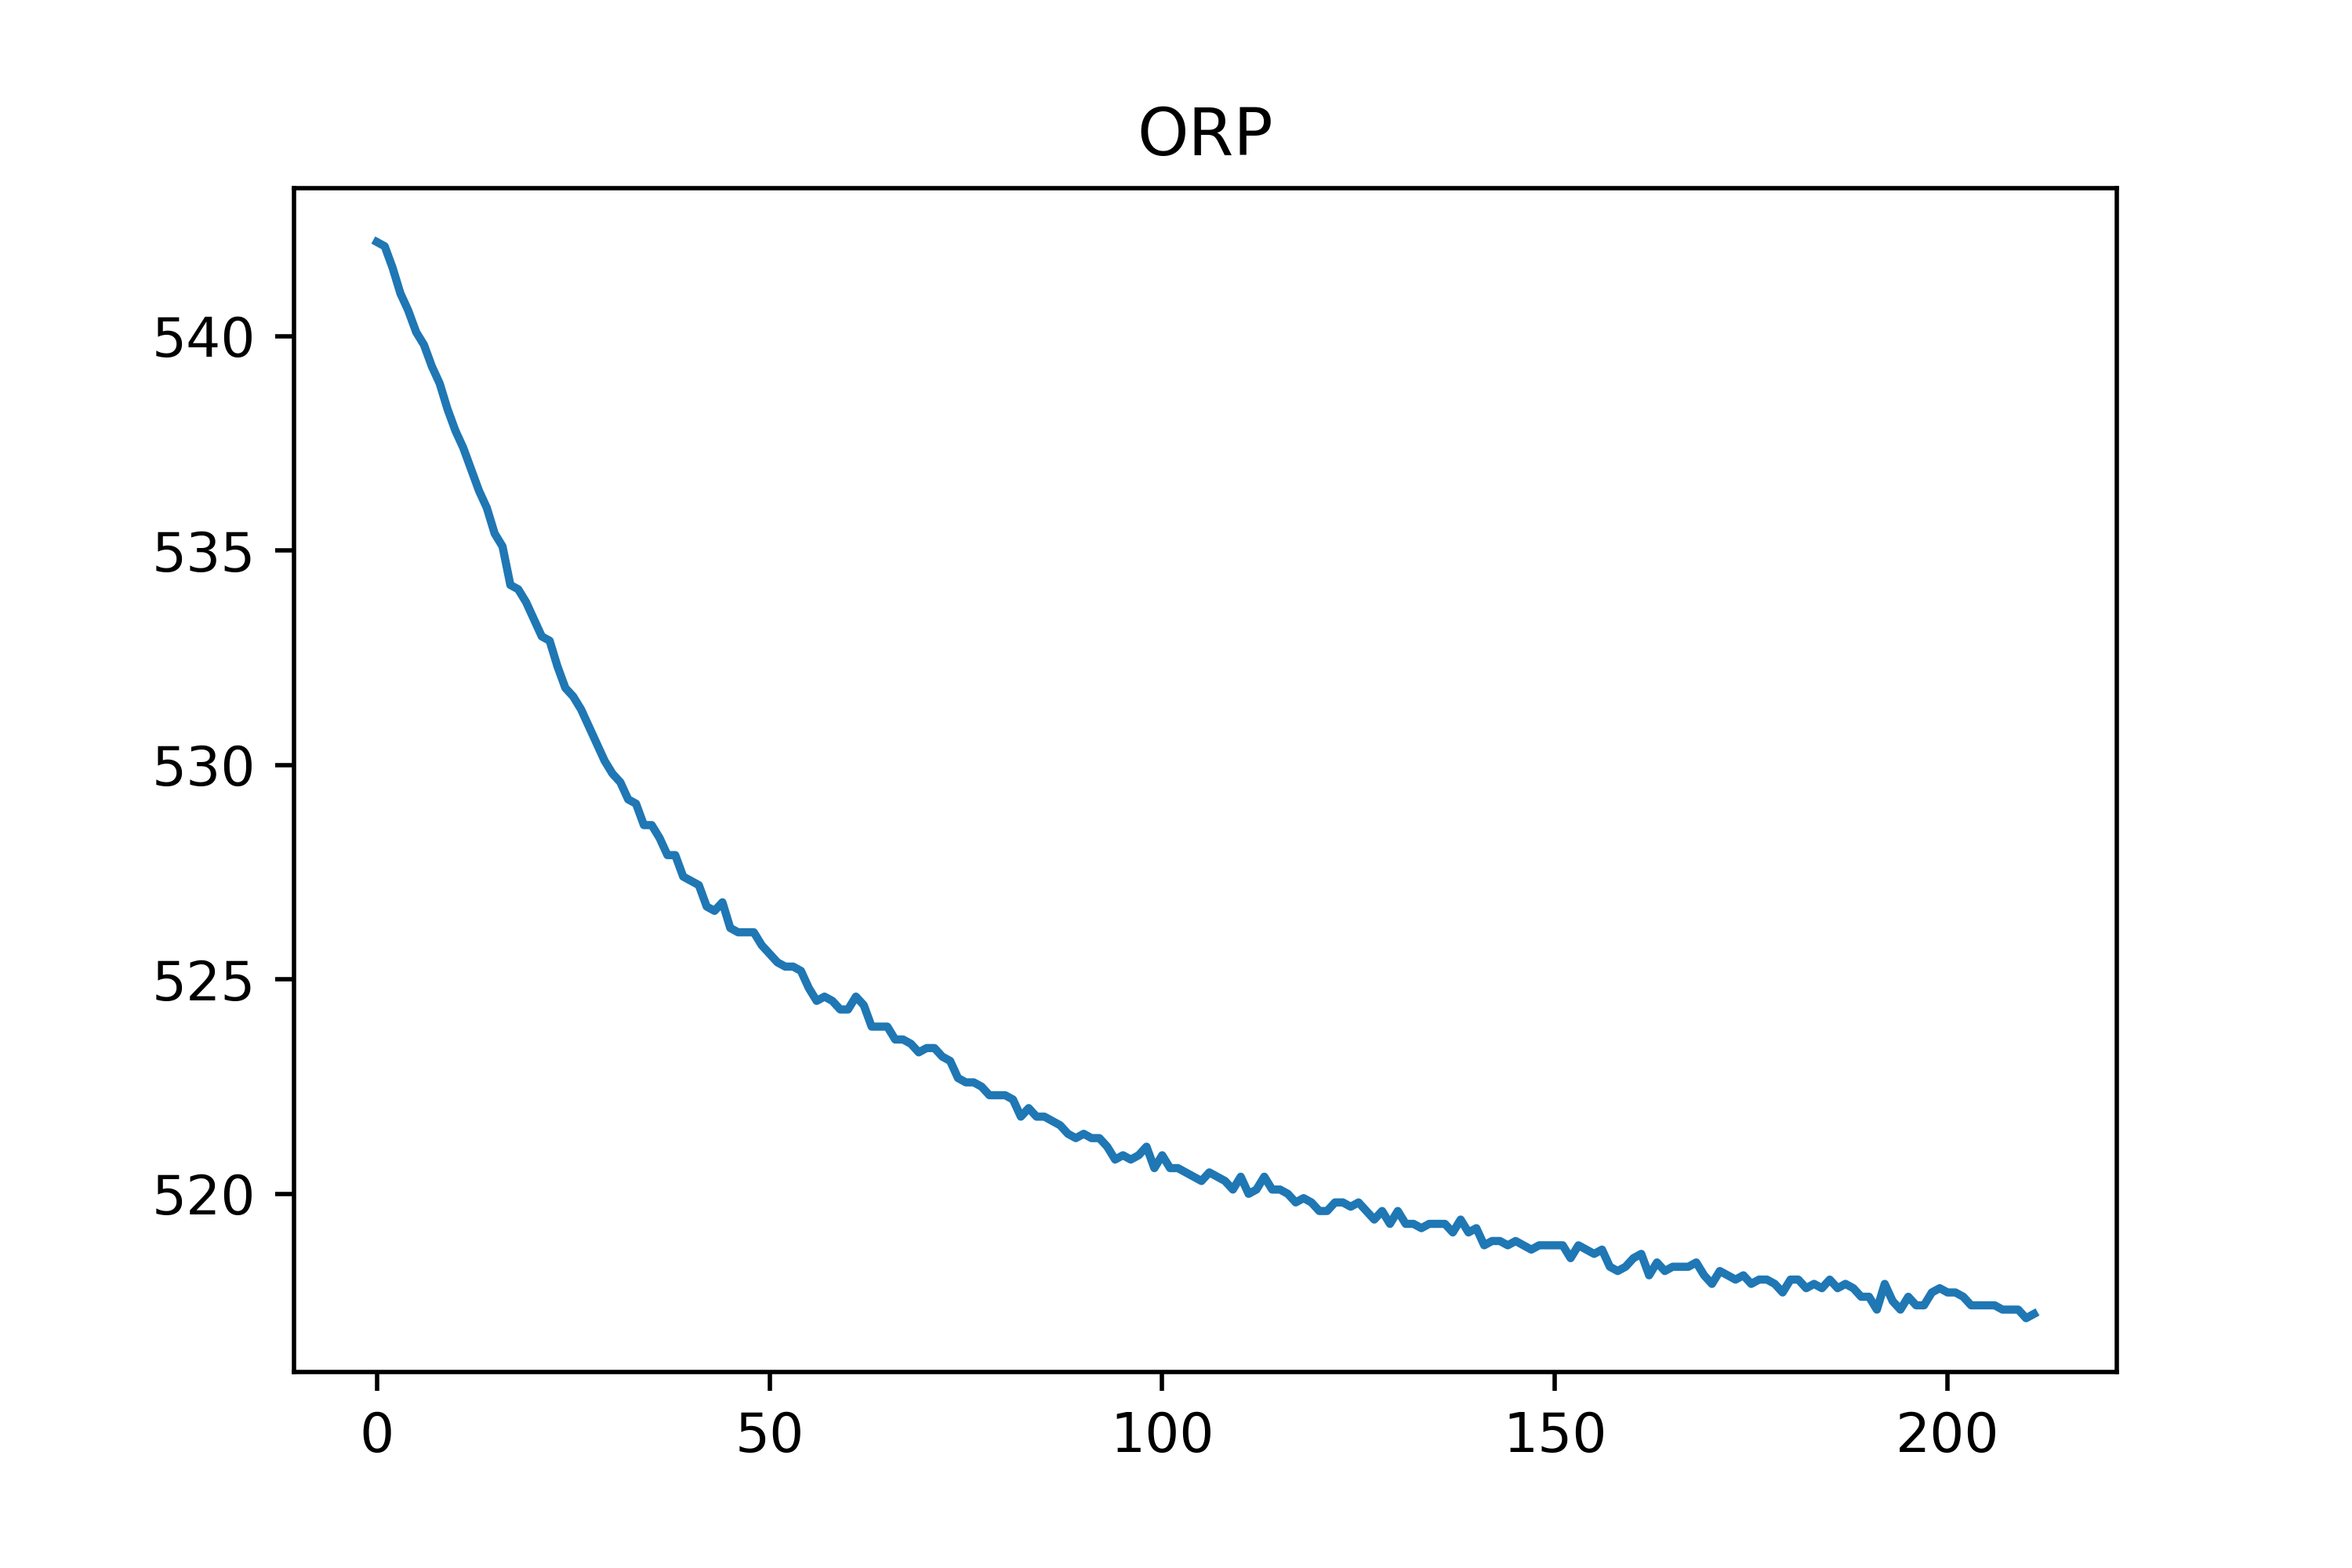
\includegraphics[scale=0.7]{imgss164.png}
	\caption{ORP en agua potable a las 4 de la tarde.}
	\label{fig:figura1000_11}
\end{figure}

En el caso de los parámetros de cloro residual y oxígeno disuelto no se registraron cambios a lo largo de los diferentes horarios muestreados. 

La novena y décima caracterizaciones fueron llevadas a cabo los días 06 y 08 de agosto respectivamente. En estos 2 experimentos se volvió a tomar muestras de las 5 etapas predeterminadas. Para el noveno y décimo experimento se solicitó que las mediciones fuesen modificadas 
para esta ocasión en específico. La petición en estas 2 caracterizaciones fue que la medición en cada una de las 5 muestras fuese de 35 minutos sin interrupciones. El objetivo de este cambio era poder observar el comportamiento de la estabilización en las mediciones para 
un periodo de tiempo más extenso, ya que los sensores utilizados, al principio de la medición, pueden presentar variaciones, pero con el paso de los minutos tanto el sensor como la muestra de agua se estabilizan, y ese fenómeno 
en específico es el que se buscaba registrar.

Sin embargo, las mediciones para la novena y décima caracterización fueron afectadas debido al nivel de contaminación que presentaba el agua cruda debido a todos los residuos generados por 
las lluvias. En estos casos, el agua cruda presentaba un color completamente café, además de tener una consistencia lodosa, respecto a lo cual en el laboratorio de muestreo se nos comentó que esas condiciones 
son principalmente ocasionadas por la filtración de arcilla. Estas condiciones generaron valores en las mediciones fuera de lo esperado, lo cual nos permite conocer que las lluvias son un factor que generan cambios que 
afectaran las mediciones con el equipo específico que hemos utilizado.

Para la décimo primera caracterización su fecha de realización fue el día 12 de noviembre de 2024. En estas fechas el agua cruda que llegaba a la planta ya no presentaba el alto nivel de contaminación que se encontró en 
las mediciones llevadas a cabo en el mes de agosto, ahora las condiciones del agua cruda eran de nuevo similares a las que se podían observar entre los meses de enero y julio. Para este experimento las variables medidas 
fueron ORP, cloro residual y oxígeno disuelto. 

En la \autoref{tab:table25000_1} se muestran los coeficientes de correlación para los datos del onceavo experimento.

\begin{table}[h]
	\begin{center}
		\begin{tabular}{| c | c | c | c |}
			\hline
			\multicolumn{4}{ |c| }{Matriz de correlación Pearson} \\ \hline
			 & DO & ORP & Cloro Residual \\ \hline
			 DO & 1 & 0.8857 & 0.9071 \\
			 ORP & 0.8857 & 1 & 0.984 \\
			 Cloro Residual & 0.9071 & 0.984 & 1 \\ \hline
		\end{tabular}
		\caption{Coeficientes de correlación para la onceava caracterización}
		\label{tab:table25000_1}
	\end{center}
\end{table}

Se observa que los coeficientes entre los parámetros significativos tienen magnitud cercana a 1, lo cual es la tendencia deseada. Este tipo de comportamiento era imposible de obtener para las mediciones del mes de agosto 
cuando las condiciones de contaminación generaban mediciones fuera de rango para las variables medidas.

La doceava caracterización se realizó el día 14 de noviembre de 2024, en la cual los parámetros medidos fueron ORP, cloro residual y oxígeno disuelto. En esta ocasión fueron realizados 3 recolecciones 
de muestras a diferentes horarios, 9 de la mañana, 1 de la tarde y 5 de la tarde, y las 3 recolecciones fueron sobre las 5 etapas del proceso predeterminadas.

Finalmente, la última caracterización fue realizada el día 19 de noviembre de 2024, en la cual se analizaron los parámetros de ORP, cloro residual y oxígeno disuelto para las 5 etapas predeterminadas.
Se realizaron 2 recolecciones de muestras en 2 horarios, a las 9 de la mañana y a la 1 de la tarde. 

En la \autoref{tab:table25000_4} se muestran los coeficientes de correlación para los datos del décimo tercer experimento.

\begin{table}[h]
	\begin{center}
		\begin{tabular}{| c | c | c | c |}
			\hline
			\multicolumn{4}{ |c| }{Matriz de correlación Pearson} \\ \hline
			 & DO & ORP & Cloro Residual \\ \hline
			 DO & 1 & 0.8264 & 0.8622 \\
			 ORP & 0.8264 & 1 & 0.9756 \\
			 Cloro Residual & 0.8622 & 0.9756 & 1 \\ \hline
		\end{tabular}
		\caption{Coeficientes de correlación para la décimo tercer caracterización}
		\label{tab:table25000_4}
	\end{center}
\end{table}

\clearpage

\section{Resultados estadísticos de los parámetros de calidad del agua}

\subsection{Parámetros descartados}

En la sección anterior se describió que inicialmente este trabajo tenía como objetivo generar modelos de clasificación de calidad del agua en el proceso de potabilización con 4 parámetros específicos, temperatura, pH, ORP y conductividad 
eléctrica. También se indicó que 3 de ellos, temperatura, pH y conductividad eléctrica, fueron descartados para modelos de clasificación debido a los resultados que generaban al realizar estadística descriptiva sobre dichas 
variables. 

En la \autoref{fig:figura1000_15} se muestra un diagrama de caja para los datos recolectados para el parámetro de pH.

\begin{figure}[h]
	\centering
	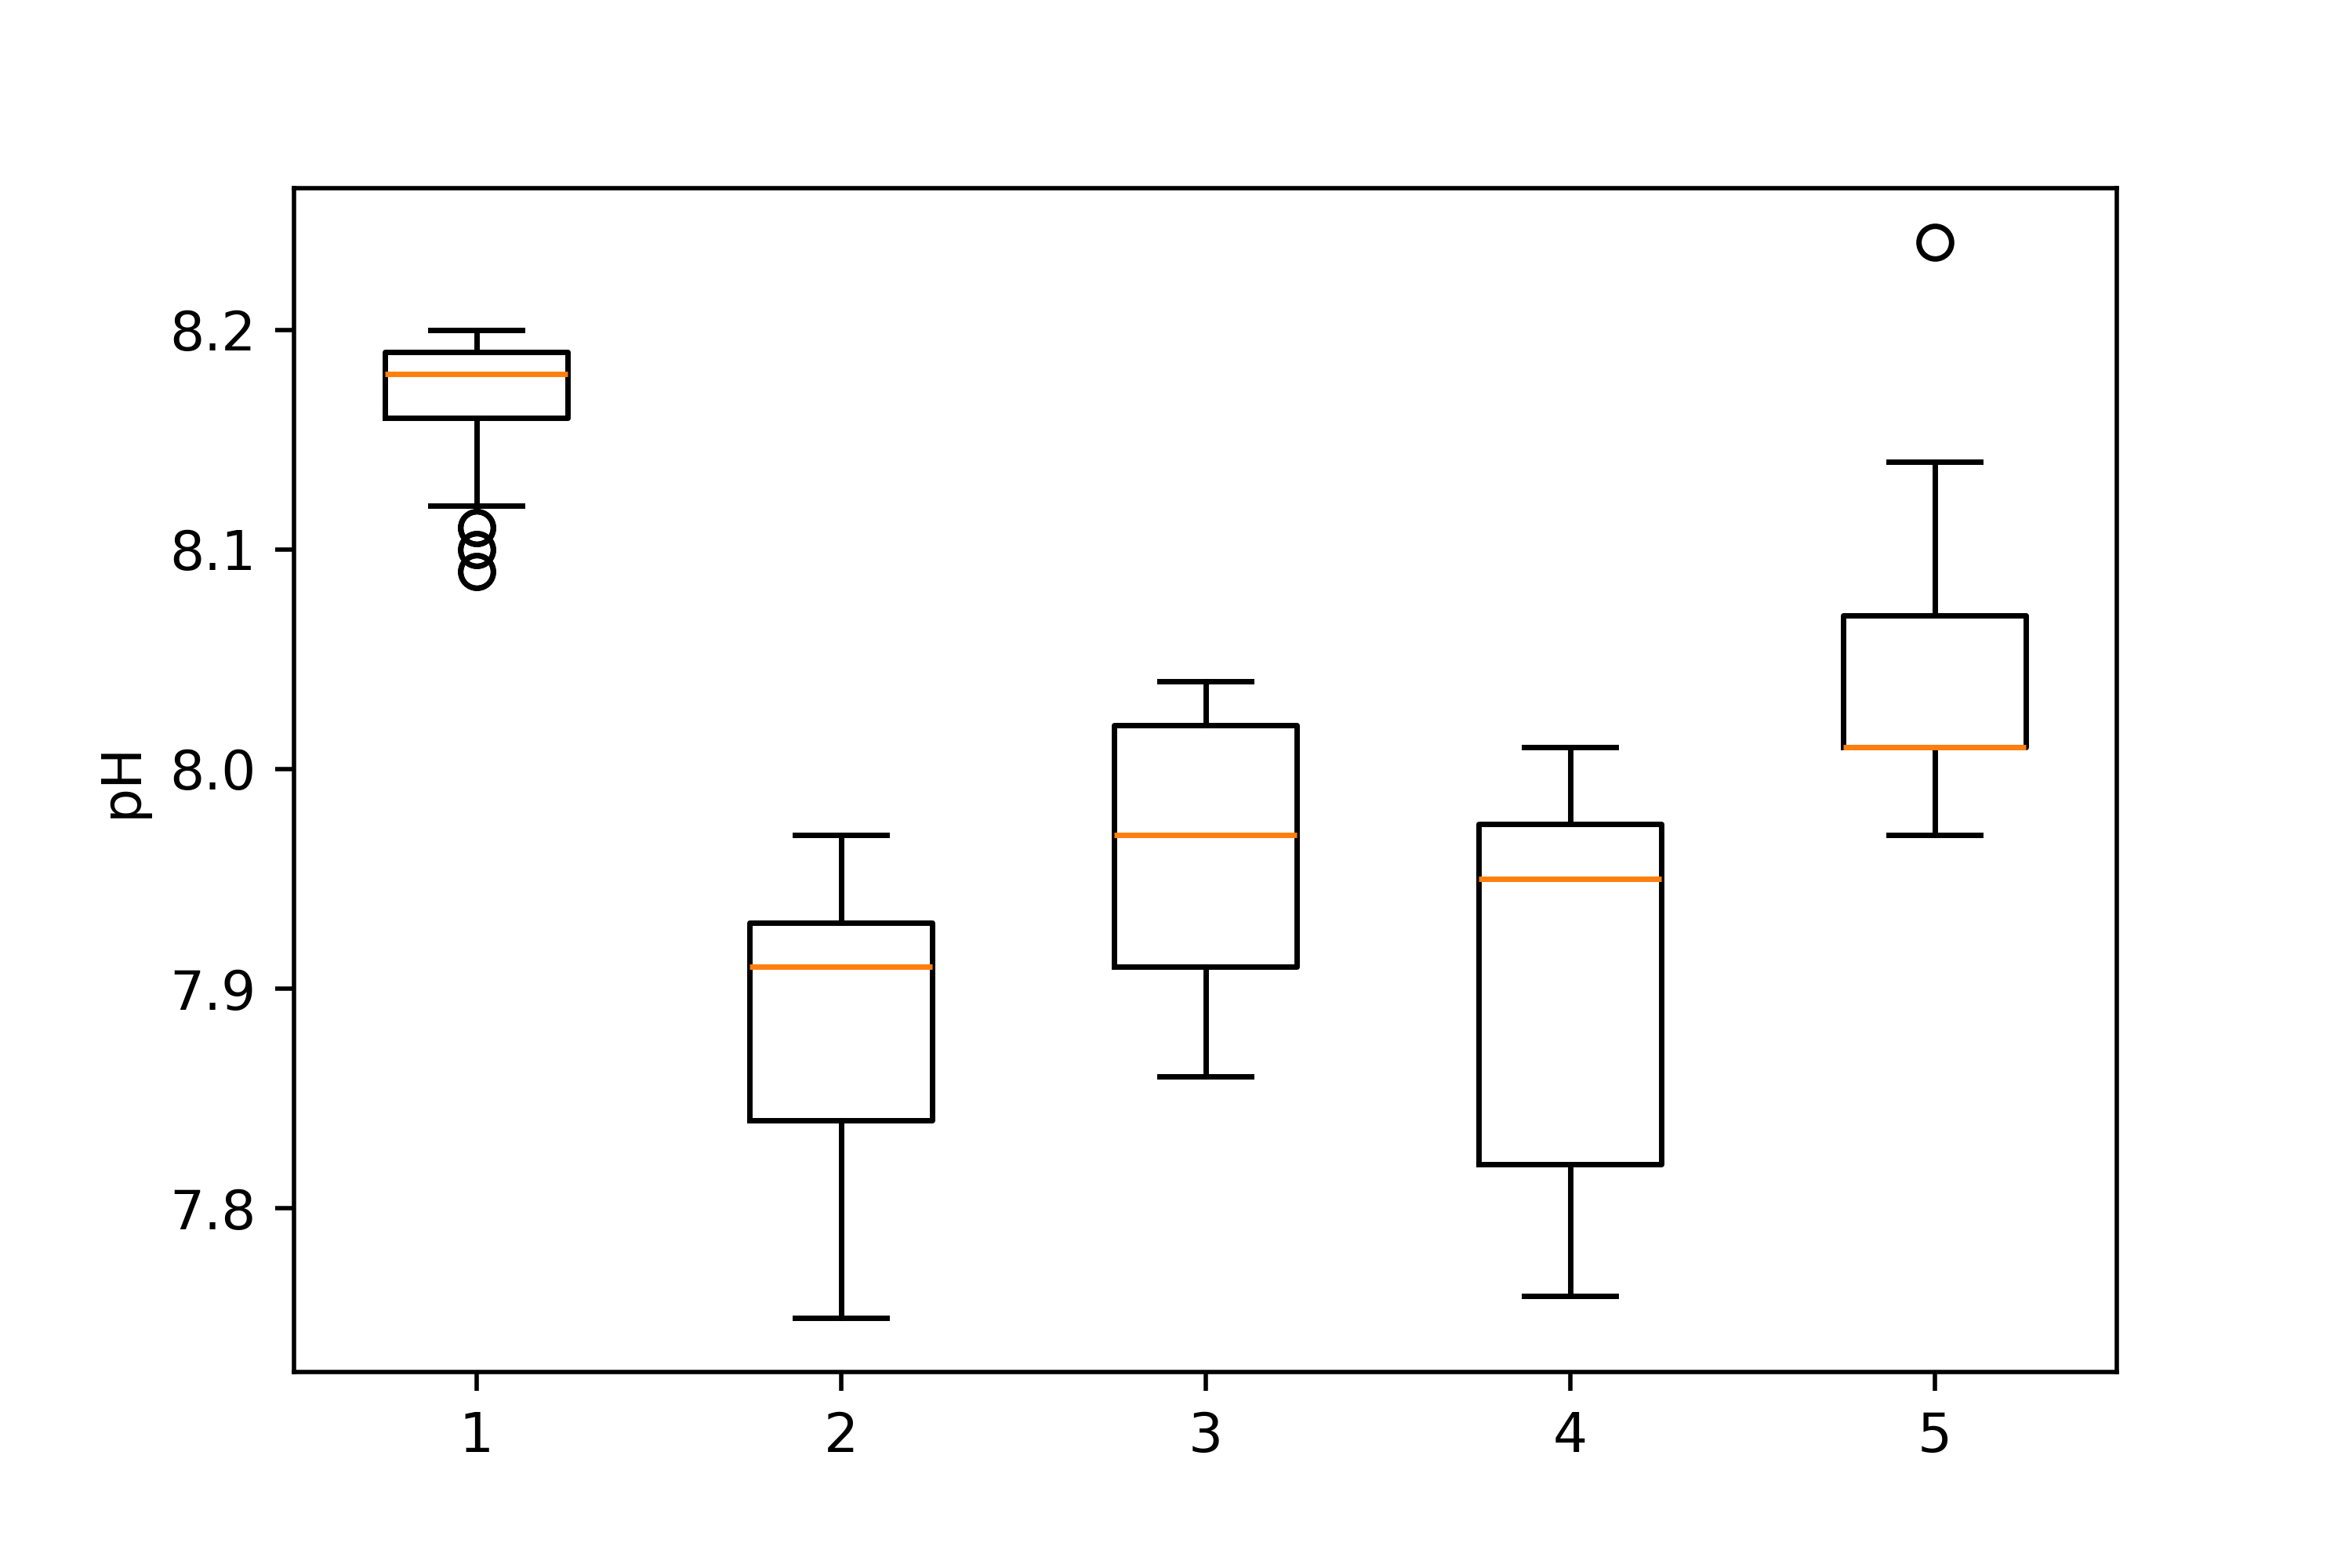
\includegraphics[scale=1.0]{imgss165.png}
	\caption{Diagrama de caja para el parámetro de pH en las 5 etapas del proceso de potabilización.}
	\label{fig:figura1000_15}
\end{figure}

En un diagrama de este tipo se representa el rango de valores que tiene una variable, en el cual las líneas superior e inferior son los valores máximo y mínimo, respectivamente; la línea marcada en color naranja representa 
la mediana de ese conjunto de datos específico, y la caja sirve para generar la separación de los datos en los 4 cuartiles correspondientes, es decir, el 25$\%$ de los datos en cada 1 de las 4 separaciones formadas por los 
límites superior e inferior, la mediana y la caja. Adicionalmente, fuera de los límites superior e inferior se marcan algunos datos en forma de círculo, los cuales se consideran datos atípicos para este caso específico.

En la \autoref{fig:figura1000_15} se enumeran 5 conjuntos de datos; el marcado como 1, corresponde a los datos de agua cruda; el marcado como 2, son los datos de tanque de mezcla rápida; el marcado como 3, son datos del 
canal sedimentador; el marcado como 4, corresponden a la salida de filtración; el marcado como 5, son los datos para el agua potable. Se puede observar que los datos para el parámetro de pH para todas las etapas del proceso 
están contenidos entre 7.8 y 8.2 en la escala estándar, recordando que la escala de pH es de 0 a 14. Por lo tanto, no resulta útil introducir a un algoritmo clasificador de red neuronal una variable que tiene una variación 
de 0.4 en magnitud para los 5 targets posibles, y además, la mayoría de los datos entre las diferentes etapas del proceso se traslapan en el mismo rango de valores entre los distintos targets del clasificador. Es decir, el 
ajuste de los pesos del clasificador incluyendo el parámetro de pH lo que ocasionaría de cierta forma es \textit{confundir} a dicho algoritmo, ya que por ejemplo un valor de pH de 7.9 puede corresponder a 3 etapas distintas,
por ejemplo, tanque de mezclado, canal sedimentador o salida de filtros, y el clasificador al final tendrá que entregar un resultado que posiblemente no corresponda correctamente con la etapa del proceso.

En la \autoref{fig:figura1000_16} se muestra el diagrama de caja para los datos recolectados para el parámetro de conductividad eléctrica.

\begin{figure}[h]
	\centering
	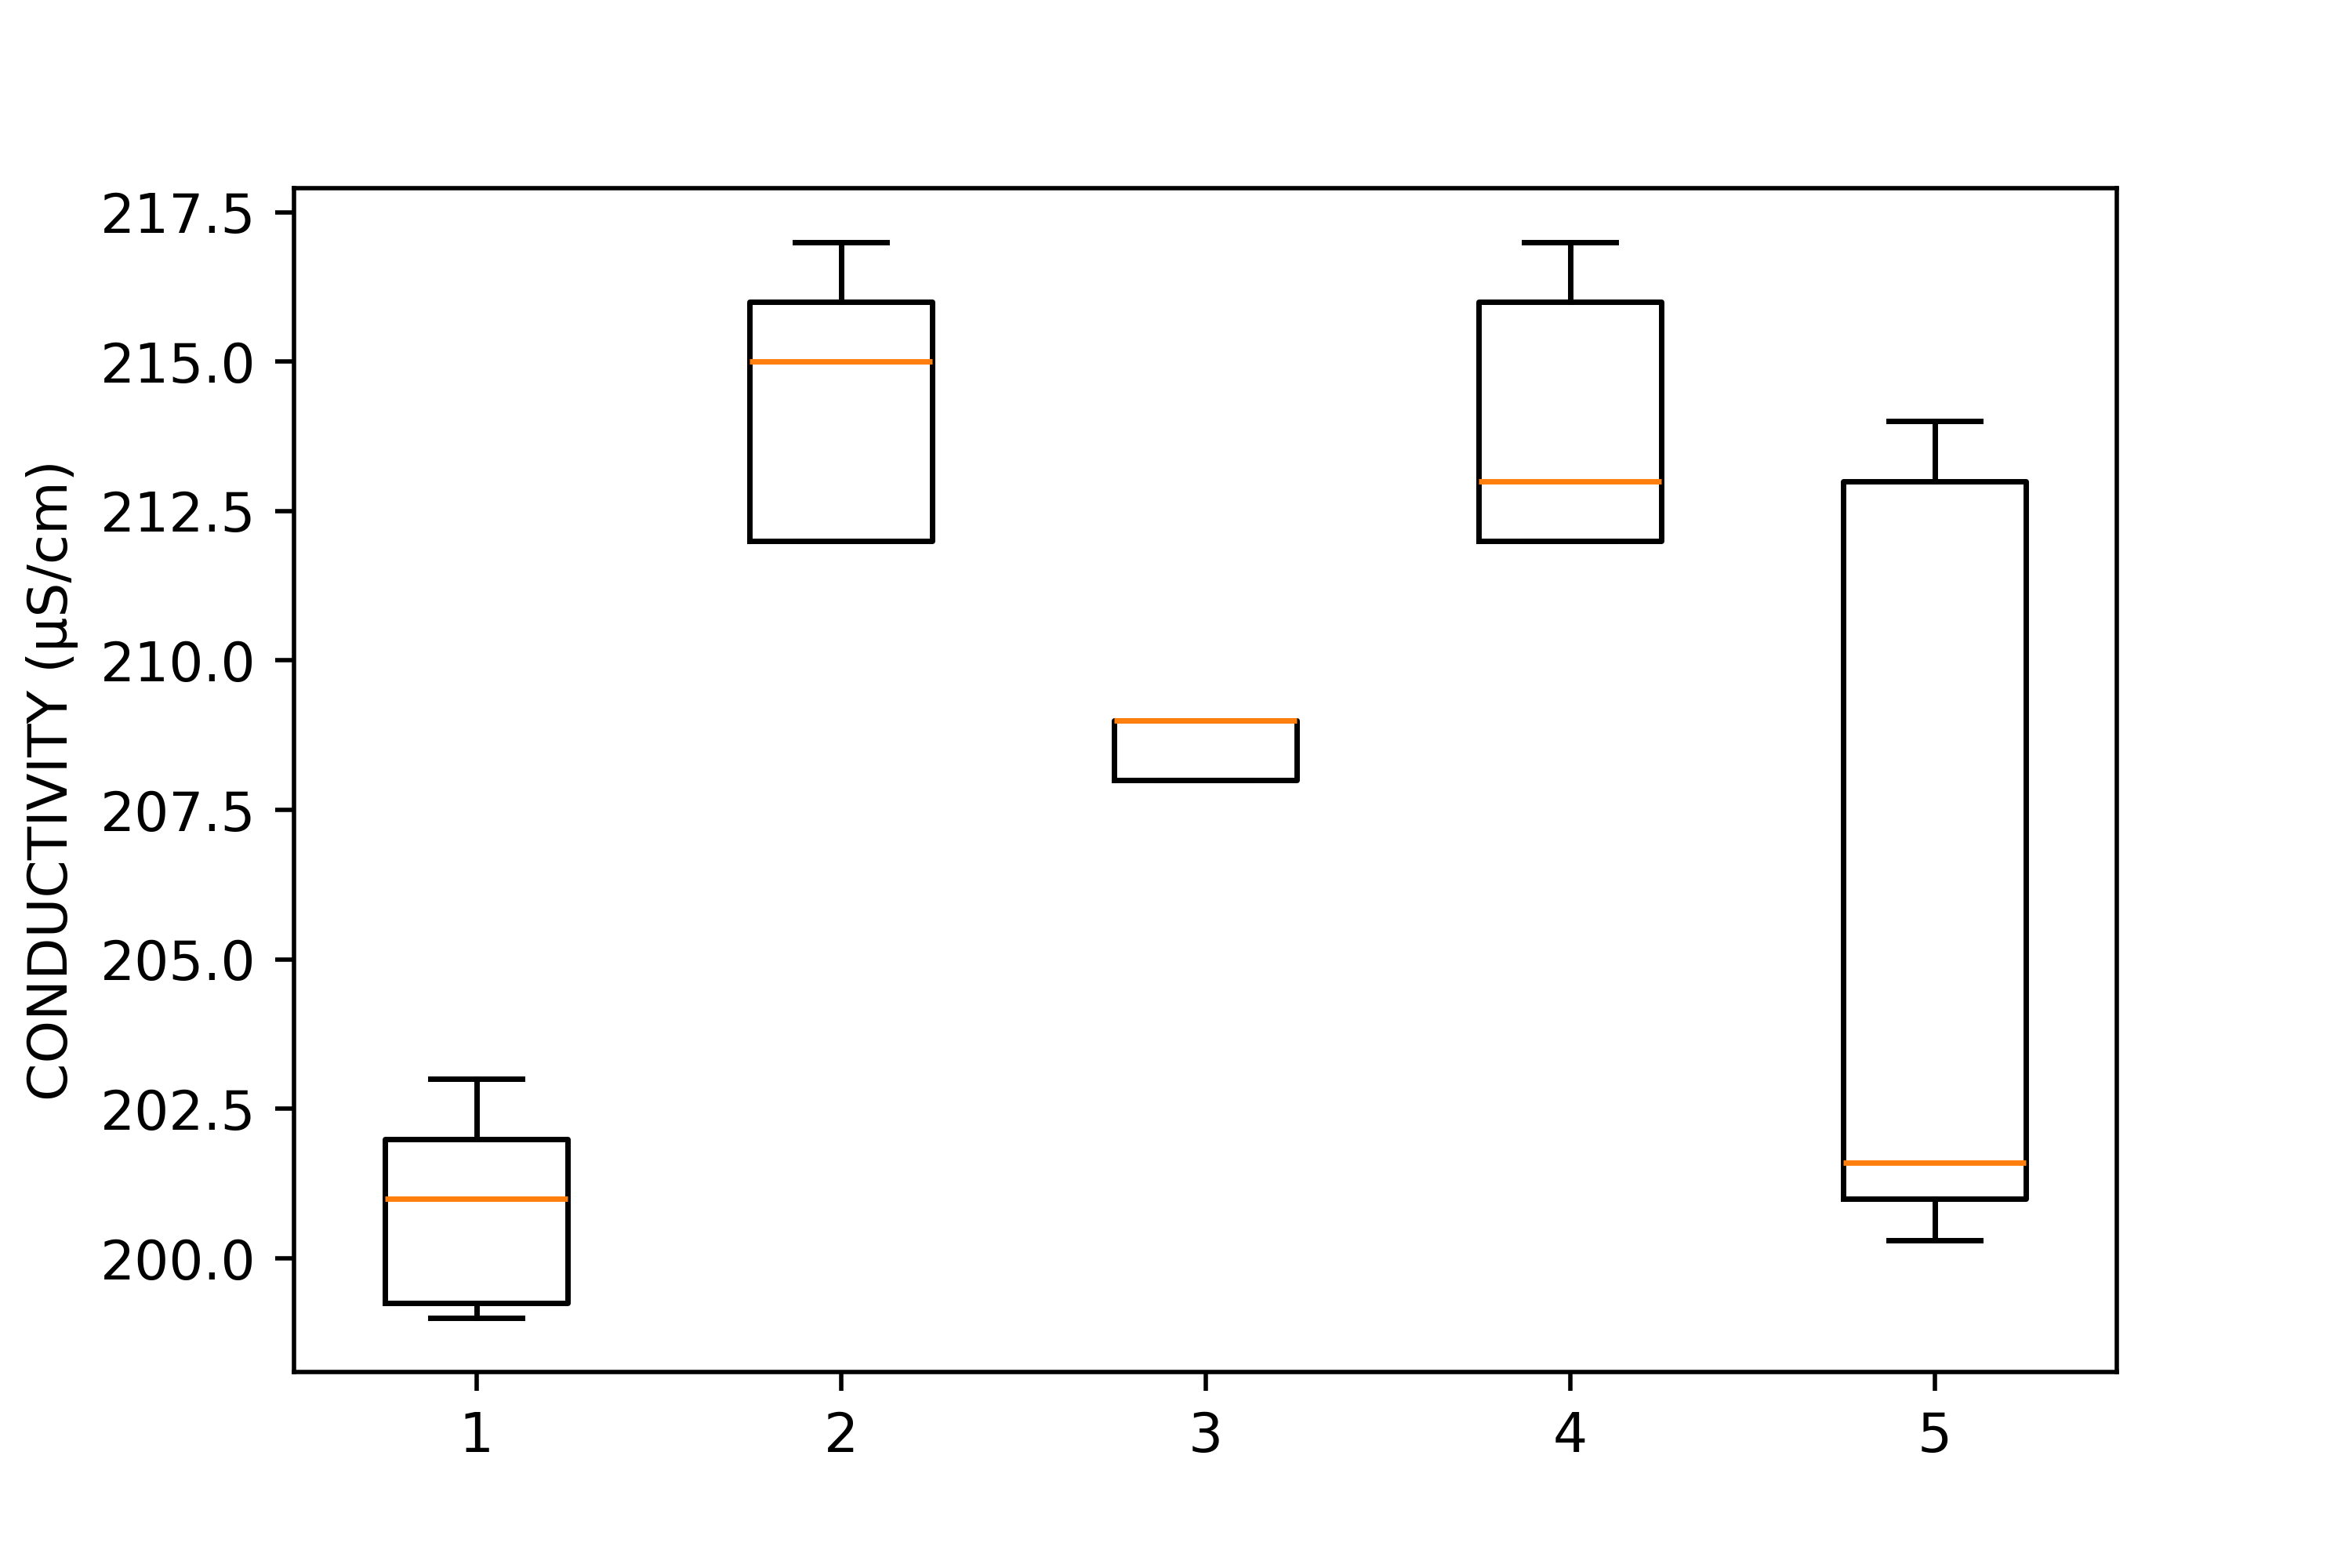
\includegraphics[scale=1.0]{imgss166.png}
	\caption{Diagrama de caja para el parámetro de conductividad eléctrica en las 5 etapas del proceso de potabilización.}
	\label{fig:figura1000_16}
\end{figure}

En la \autoref{fig:figura1000_16} se visualizan los datos de conductividad en las 5 etapas analizadas en el proceso de potabilización. Como primer argumento para las conclusiones con esta variable es el hecho de que los 
datos correspondientes a la etapa de tanque de mezclado rápido y la etapa de salida de filtración, ambos casos caen ene el mismo rango. El segundo argumento tiene que ver con el mismo hecho, sólo que ahora para los datos 
de la etapa de canal sedimentador y la etapa de agua potable, en cuyo caso todos los datos medidos para la etapa de canal sedimentador caen dentro del rango de valores más amplio que abarca esta variable para la etapa de 
agua potable. Por lo tanto, nuevamente se tiene el caso de traslape de valores entre los diferentes targets posibles para el clasificador, lo cual se sabe que la inclusión de una variable con estas condiciones lo que ocasiona 
es que el modelo se aleje más de las condiciones ideales de lograr una función de costo de magnitud 0 después del entrenamiento.

En la \autoref{fig:figura1000_17} se muestra el diagrama de caja para el parámetro de temperatura.

\begin{figure}[h]
	\centering
	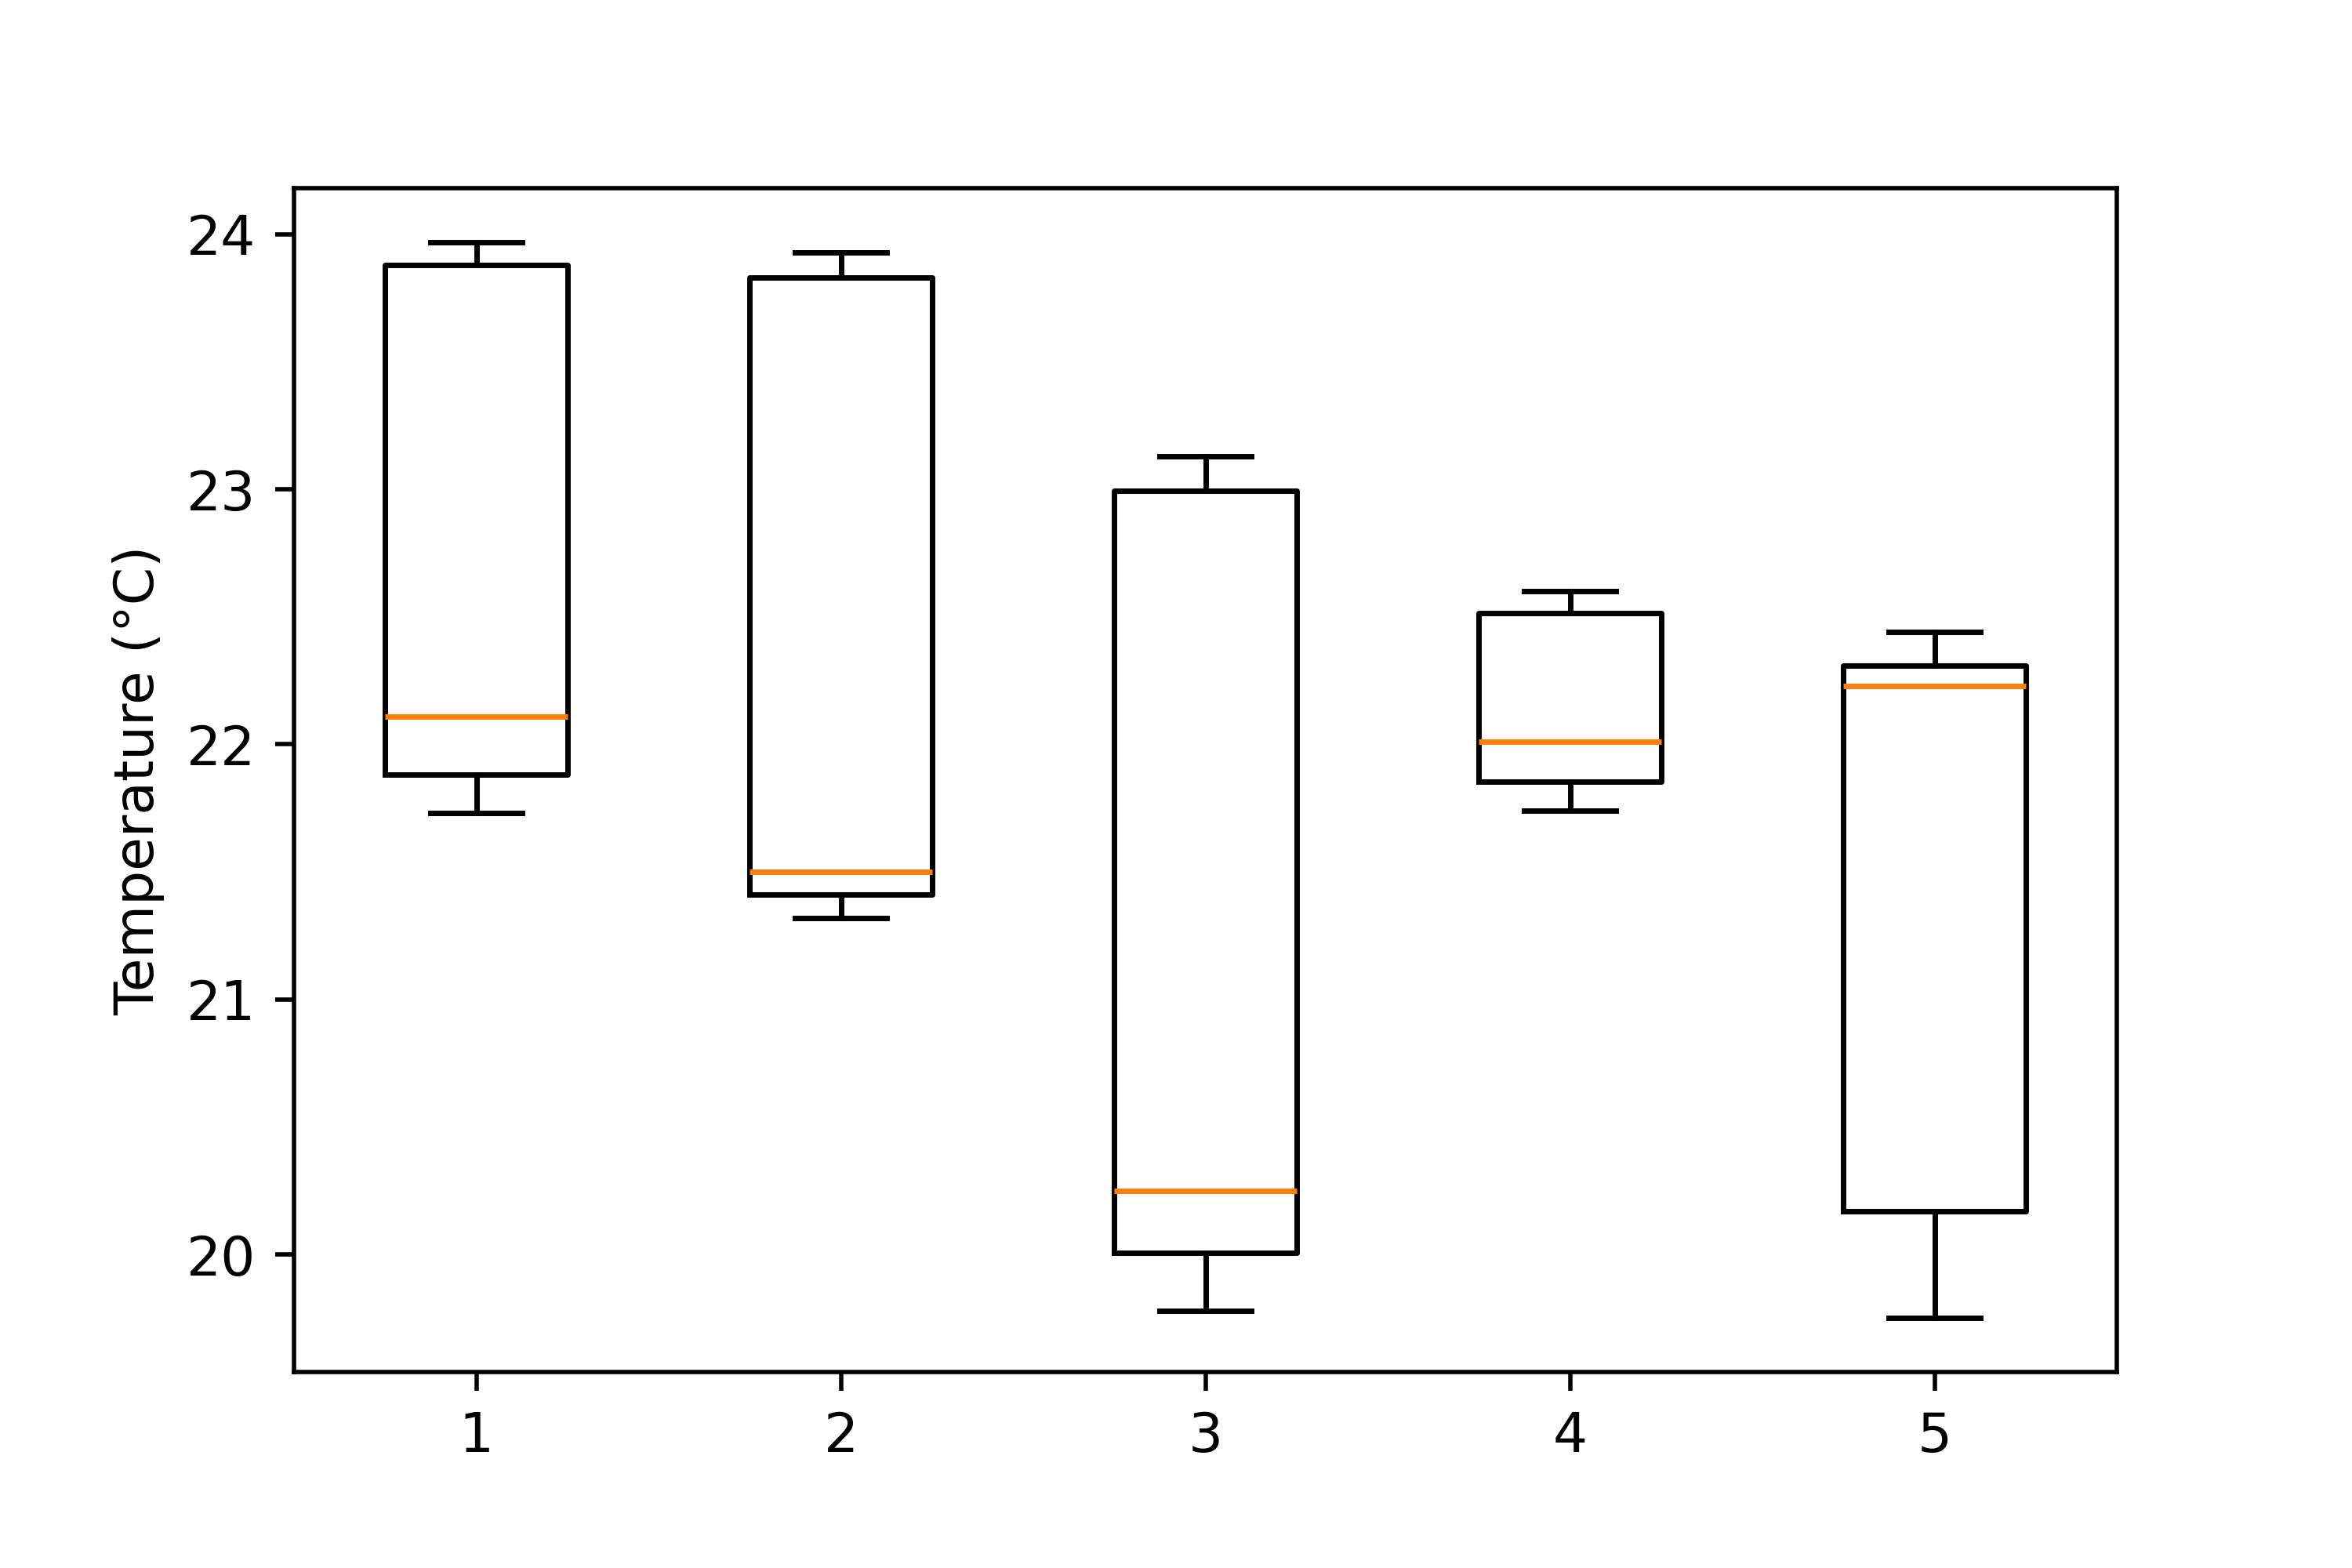
\includegraphics[scale=1.0]{imgss167.png}
	\caption{Diagrama de caja para el parámetro de temperatura en las 5 etapas del proceso de potabilización.}
	\label{fig:figura1000_17}
\end{figure}

Para la variable de temepratura, en la \autoref{fig:figura1000_17} se pueden ver casos similares a los dados con el pH y conductividad; las 5 etapas del proceso comparten prácticamente el mismo rango de valores, por lo cual 
no es posible identificar una etapa específica con el uso de este parámetro, además de que también la diferencia en magnitud entre los valores mínimo y máximo registrados es muy pequeña. Para el caso de la temperatura en 
la revisión del estado del arte se encontraron diversos estudios donde se establecía dicho parámetro como de importancia en modelos de IA para análisis de calidad del agua, sin embargo, en nuestro caso de estudio ha resultado 
inútil esta variable principalmente a causa de que todas la muestras de agua recolectadas están dentro un espacio en el cual se puede considerar que la temperatura es constante, por lo cual el fenómeno de equilibrio térmico 
lleva a que el agua que se puede encontrar en la planta de potabilización no presente diferencias de magnitud importante en su temperatura, a pesar de que las muestras correspondan a diferentes fases del proceso de tratamiento.

\clearpage

\subsection{Parámetros significativos}

La implementación de redes neuronales para estimación de calidad fue realizada mediante 3 parámetros, ORP, cloro residual y oxígeno disuelto, las cuales son las variables que presentan un comportamiento viable para formar 
con ellas un conjunto de datos para entrenamiento y validación.

En la \autoref{fig:figura1000_18} se muestra el diagrama de caja para los datos recolectados durante el año 2024 para el parámetro de ORP.

\begin{figure}[h]
	\centering
	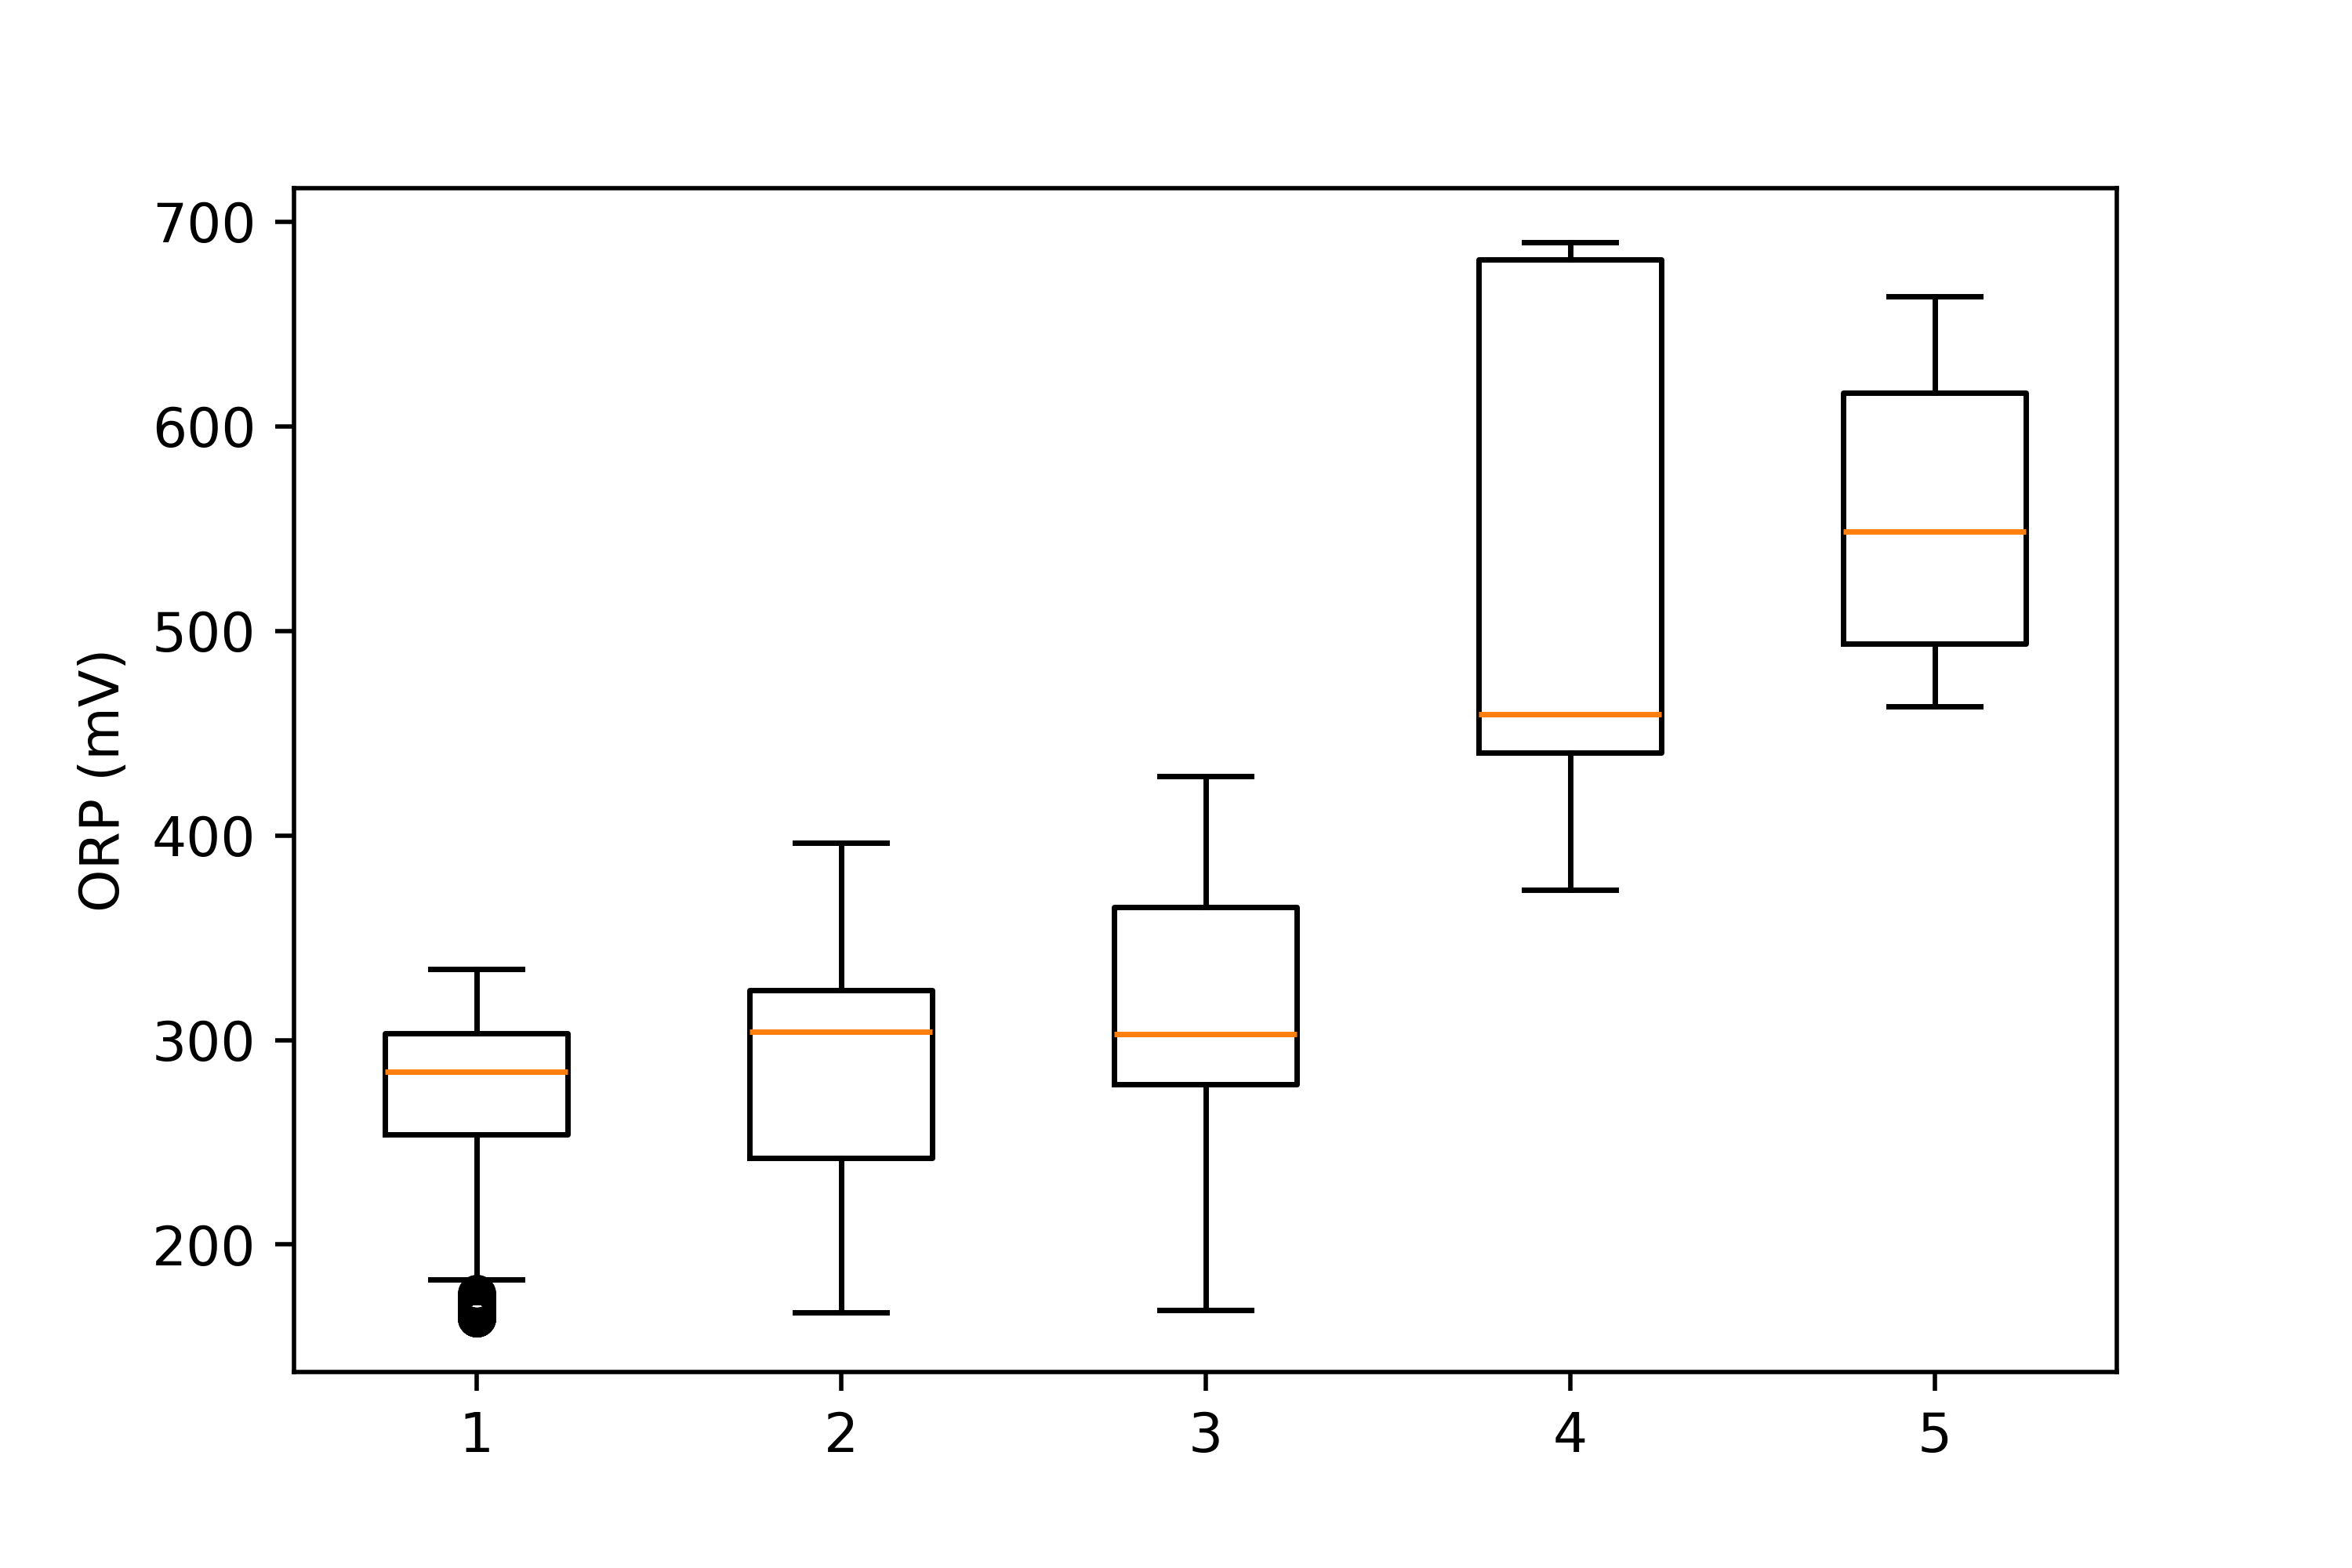
\includegraphics[scale=1.0]{imgss168.png}
	\caption{Diagrama de caja para el parámetro de ORP.}
	\label{fig:figura1000_18}
\end{figure}

\clearpage

La \autoref{fig:figura1000_19} muestra el diagrama de caja correspondiente a la variable de cloro residual.

\begin{figure}[h]
	\centering
	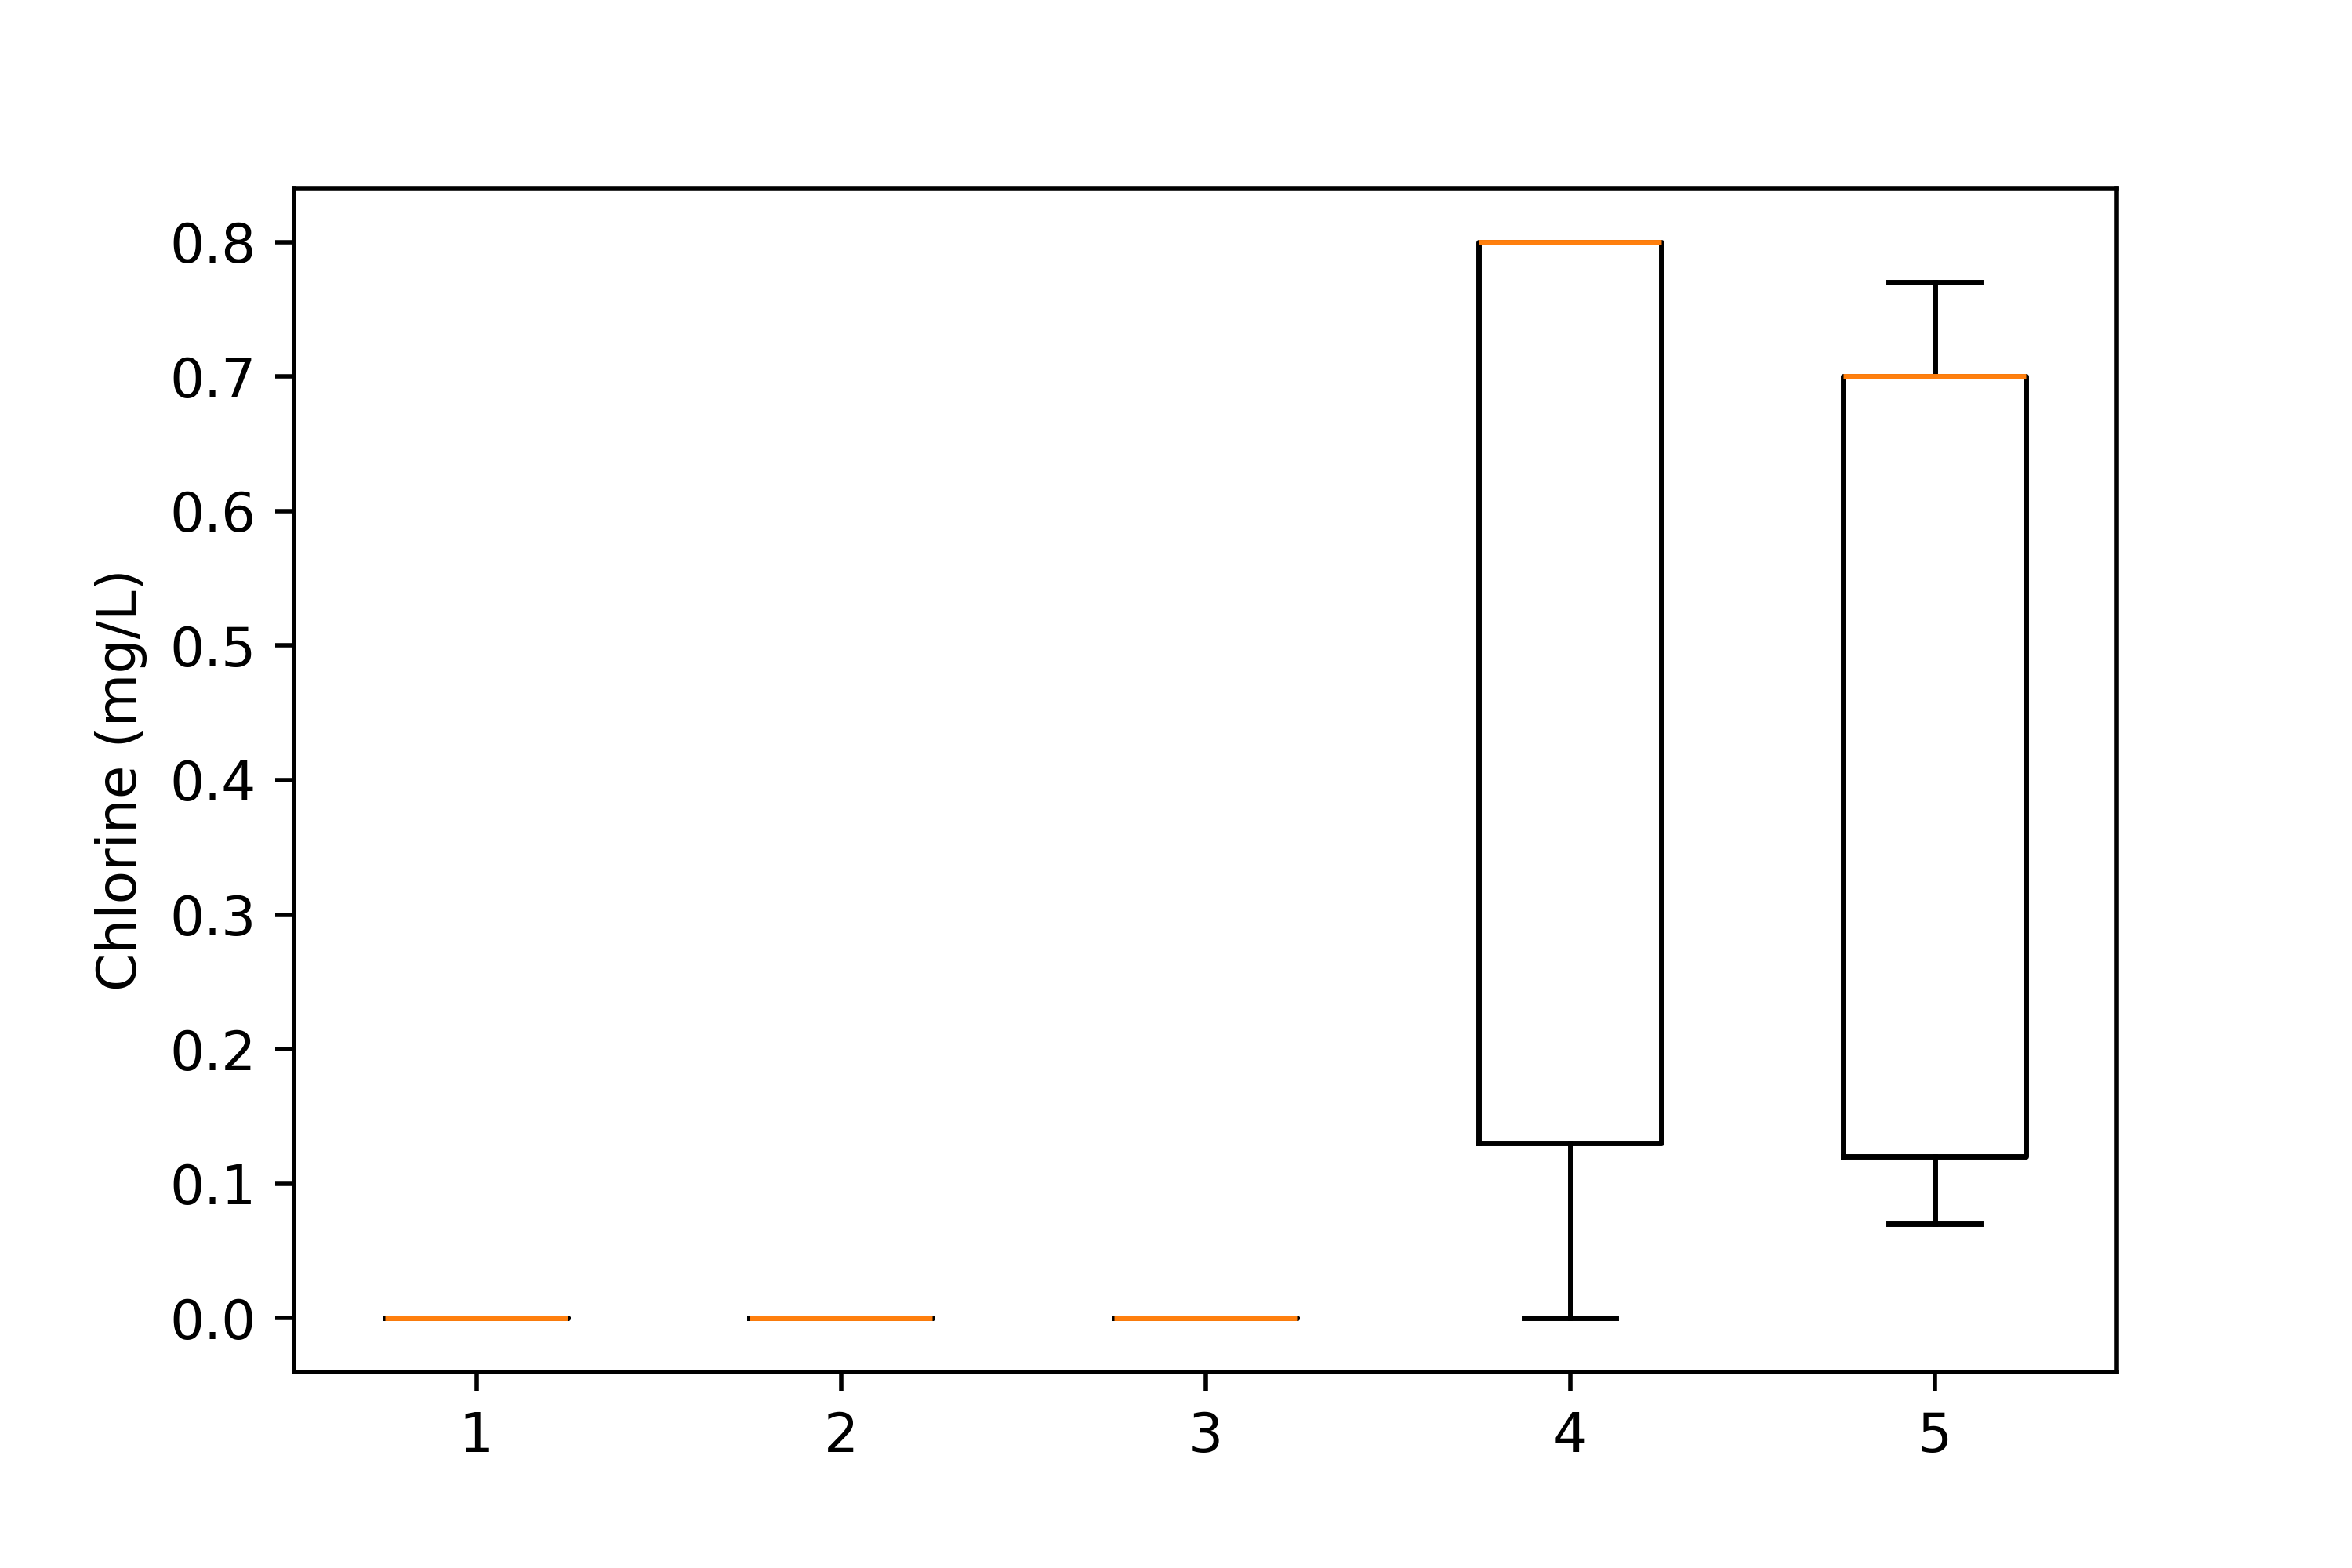
\includegraphics[scale=1.0]{imgss169.png}
	\caption{Diagrama de caja para el parámetro de cloro residual.}
	\label{fig:figura1000_19}
\end{figure}

\clearpage

Finalmente, la \autoref{fig:figura1000_20} muestra el diagrama de caja para el parámetro de oxígeno disuelto.

\begin{figure}[h]
	\centering
	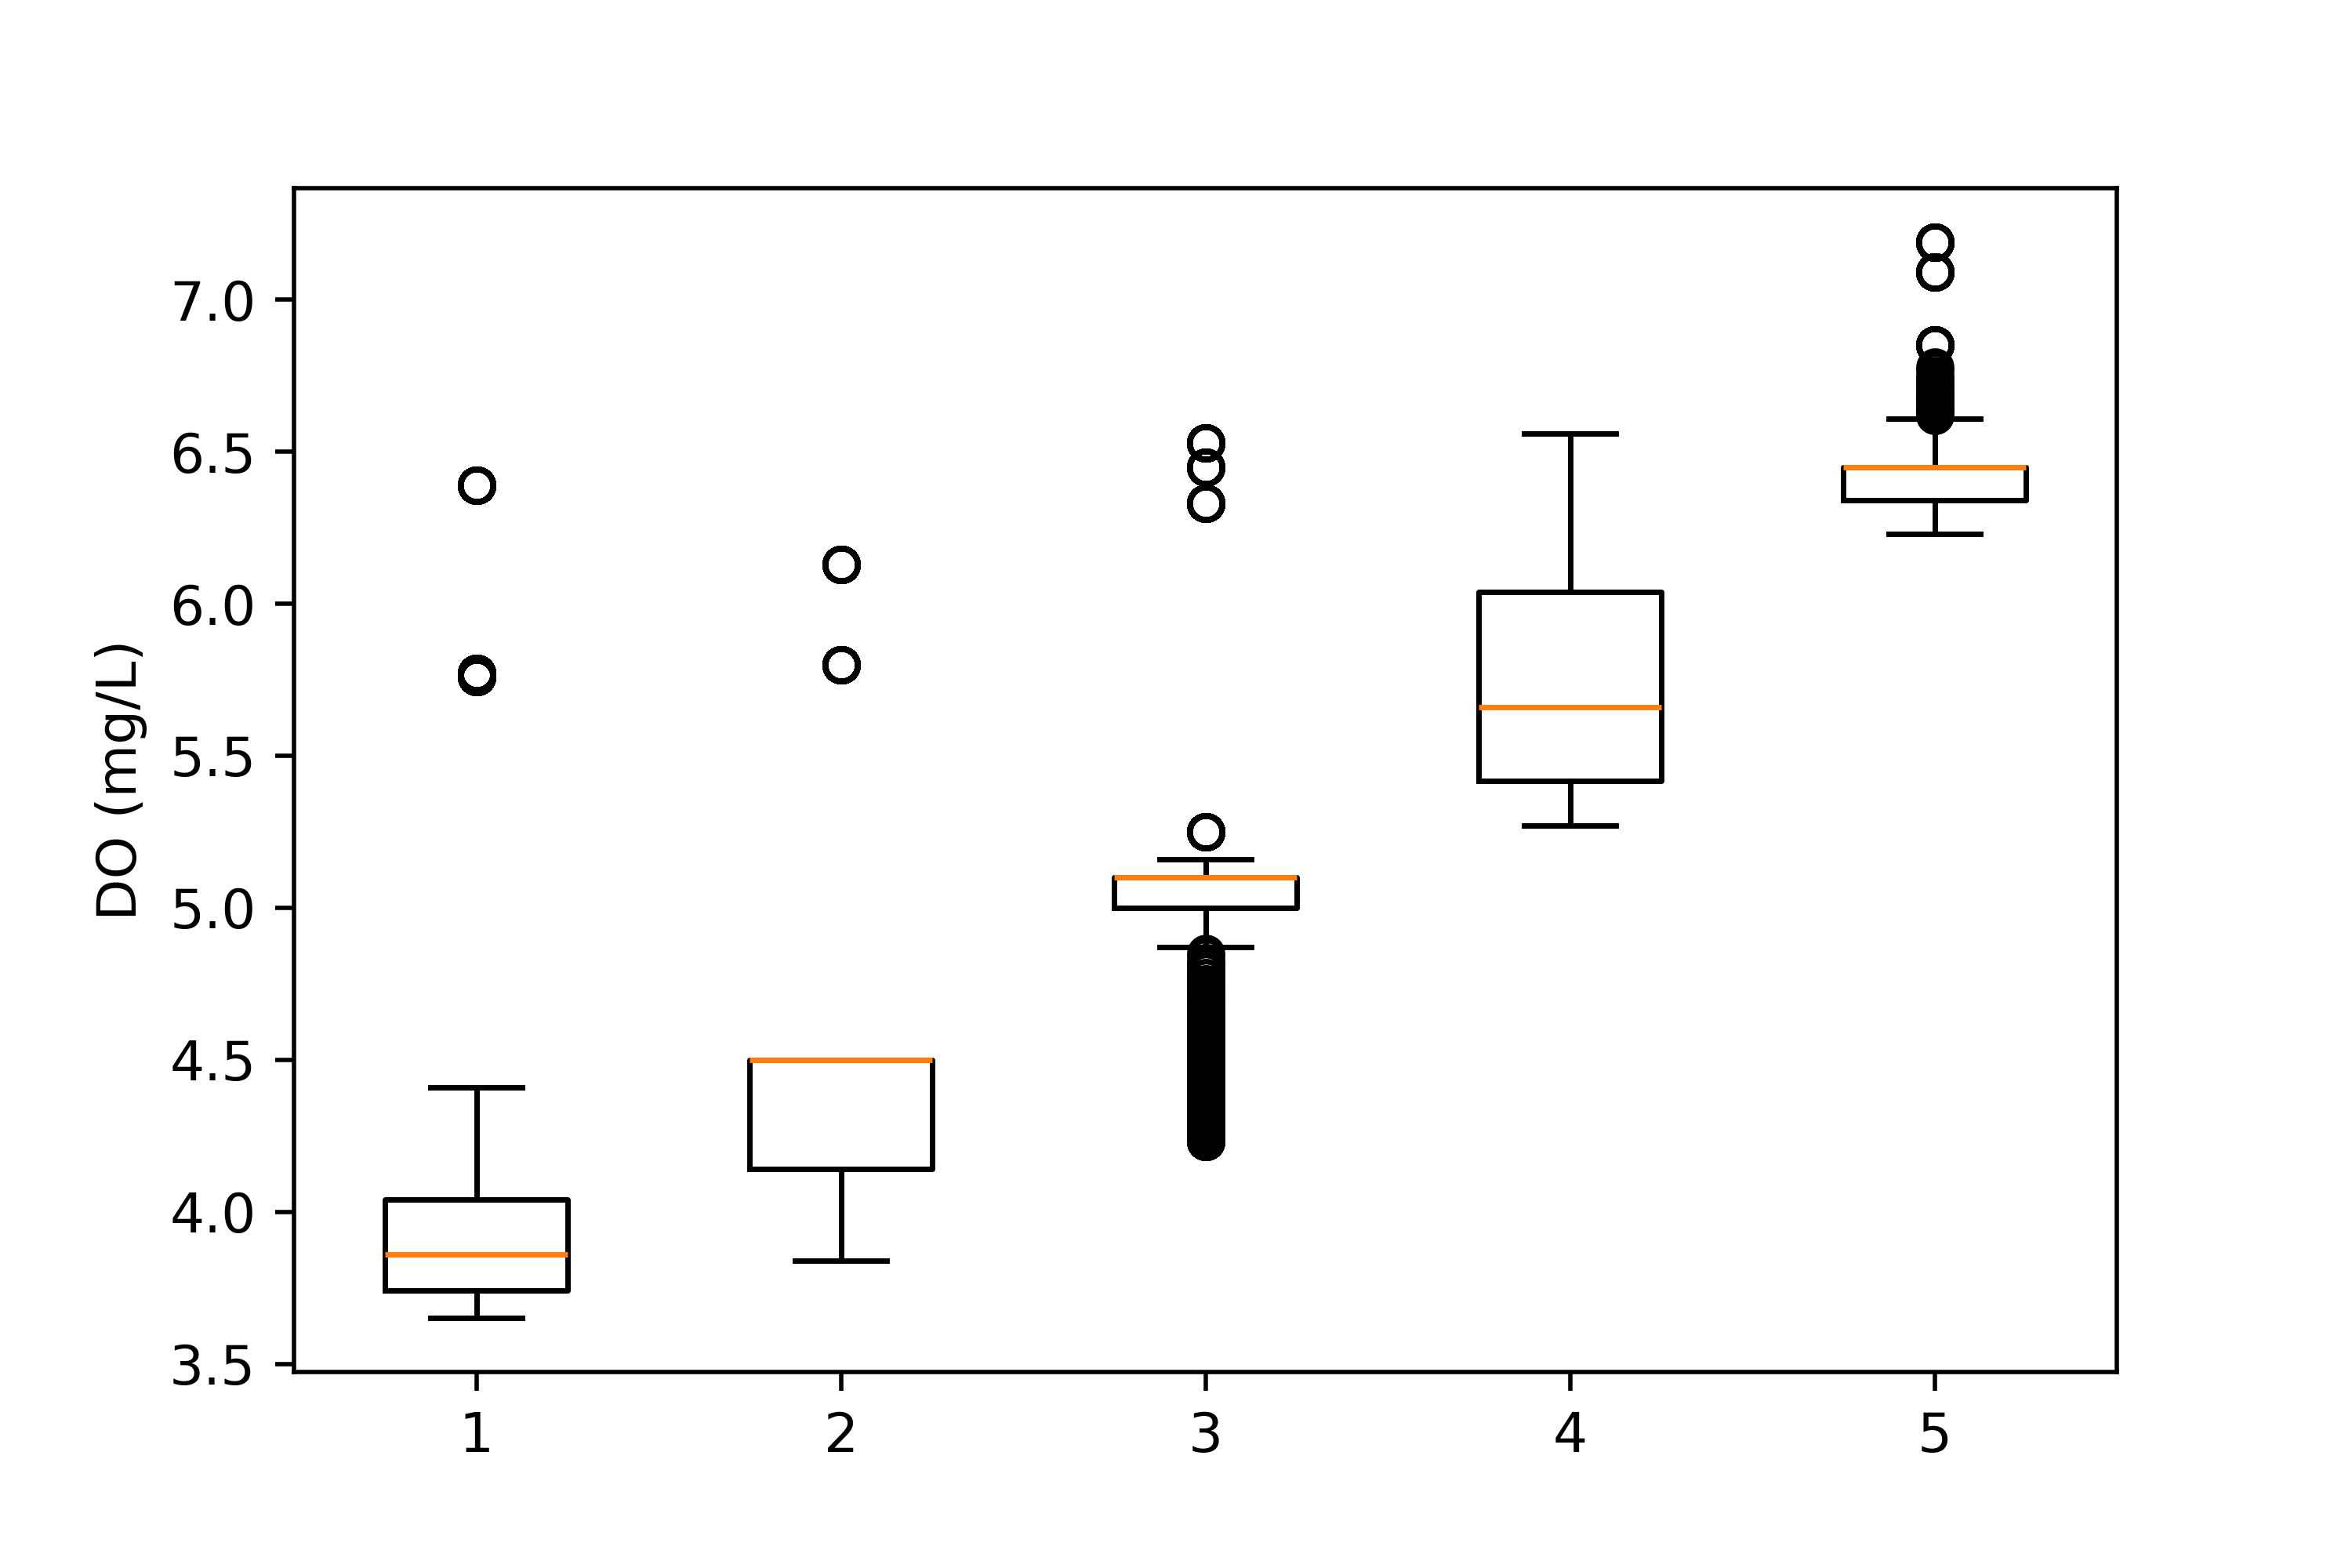
\includegraphics[scale=1.0]{imgss170.png}
	\caption{Diagrama de caja para el parámetro de oxígeno disuelto.}
	\label{fig:figura1000_20}
\end{figure}

Primeramente, en la \autoref{fig:figura1000_18} el diagrama de ORP muestra una buena aproximación del comportamiento teórico deseable para una aplicación de este tipo. Tanto en el estado del arte como en el laboratorio de 
muestreo del OOAPAS se estableció que el comportamiento esperado para el parámetro de ORP es un incremento en su magnitud conforme mejora la calidad del agua, es decir, conforme el líquido presenta meyor grado de tratamiento.
El diagrama de caja muestra precisamente una tendencia incremental conforme se avanza a través de la etapas de potabilización, observándose principalmente un cambio importante en la magnitud del valor de ORP entre las etapas 
de canal sedimentador y salida de filtración. Este cambio lo que nos puede dar como conclusión sobre este proceso de potabilización en específico es que justamente al pasar por la última etapa de filtrado del proceso, es 
cuando el agua comienza a adquirir una característica de potencial antimicrobiano al empezar el parámetro de ORP a tomar valores en el rango de los 600mV o mayor.

En el diagrama de caja de la \autoref{fig:figura1000_19} correspondiente a cloro residual se tiene un comportamiento marcado claramente, es decir, en las etapas de agua cruda, tanque de mezcla rápida y canal sedimentador 
no se tiene presencia de remanentes del desinfectante; es hasta las últimas 2 etapas analizadas cuando el equipo de medición logra registrar la presencia de esta sustancia, lo cual es imprescindible que a la salida del 
proceso exista una cierta cantidad, para poder cumplir con la regulación sanitaria correspondiente que indica que el rango permisible es de 0.2mg/L a 1.5mg/L para agua potable a la salida del proceso.

Por último, para el diagrama mostrado en la \autoref{fig:figura1000_20} correspondiente a oxígeno disuelto, en este caso también se tiene una tendencia incremental de la magnitud de la variable conforme hay mejoras en la 
calidad del agua, lo que nos indica que para este proceso específico esta variable presenta la tendencia de incrementarse conforme el líquido viaja a través de las diferentes fases que se tienen en la planta de potabilización.
También es importante resaltar que el diagrama muestra, especialmente para las primeras 3 etapas analizadas, varios datos atípicos los cuales corresponden puntualmente a algunas de las mediciones efectuadas en las últimas 
caracterizaciones llevadas a cabo en el mes de noviembre. 

En la \autoref{tab:table25000_9} se muestran los coeficientes de correlación para los datos de parámetros significativos.

\begin{table}[h]
	\begin{center}
		\begin{tabular}{| c | c | c | c |}
			\hline
			\multicolumn{4}{ |c| }{Matriz de correlación Pearson} \\ \hline
			 & ORP & Cloro Residual & Oxígeno Disuelto \\ \hline
			 ORP & 1 & 0.7936 & 0.7198 \\
			 Cloro Residual & 0.7936 & 1 & 0.5801 \\
			 Oxígeno Disuelto & 0.7198 & 0.5801 & 1 \\ \hline
		\end{tabular}
		\caption{Coeficientes de correlación para los datos del año 2024}
		\label{tab:table25000_9}
	\end{center}
\end{table}

En estos resultados de correlación el coeficiente que está un poco más lejano al valor de 1 de correlación lineal perfecta es el coeficiente dado por la relación entre las variables de cloro residual y oxígeno disuelto. 
Este valor un poco más alejado de 1 se debe principalmente a que el parámetro de oxígeno disuelto sí presenta una tendencia incremental durante todo el proceso, mientras que la variable de cloro residual no tiene cambios 
en las primeras 3 etapas analizadas, es hasta la transición entre el canal sedimentador y la salida de filtración que hay cambios para este parámetro. Esta es la razón de que el coeficiente tiene magnitud menor, es decir,
que la variable de oxígeno disuelto tiene un incremento de cierta manera uniforme a lo largo de todas las etapas, mientras que el parámetro de cloro residual no tiene crecimiento a través de las 5 etapas analizadas, únicamente 
las últimas 2 etapas lo tienen, por lo cual la tendencia no es exactamente igual para ambas variables y consecuentemente su coeficiente de correlación decrementa su magnitud.

\clearpage

\subsection{Parámetros significativos con datos atípicos de época de lluvias}

Los resultados mostrados en la \textit{Sección 6.2.2 Parámetros significativos}, se indicó que eran todos los datos recolectados durante el total de las caracterizaciones, y que ese conjunto de datos en específico era el 
usado posteriormente para los modelos de redes neuronales. Sin embargo, ese conjunto de datos no incluye los valores recolectados en el mes de agosto cuando el agua que llegaba a la planta de potabilización presentaba niveles 
muy elevados de contaminación debido a las lluvias de temporada. En esta sección se muestran los mismos resultados estadísticos de la sección anterior pero agregando al conjunto de datos la información correspondiente a 
ese mes de agosto, para hacer la comparativa y ver los efectos que se generan en los resultados.

En la \autoref{tab:table25000_10} se muestran los coeficientes de correlación correspondientes.

\begin{table}[h]
	\begin{center}
		\begin{tabular}{| c | c | c | c |}
			\hline
			\multicolumn{4}{ |c| }{Matriz de correlación Pearson} \\ \hline
			 & ORP & Cloro Residual & Oxígeno Disuelto \\ \hline
			 ORP & 1 & 0.7098 & 0.7085 \\
			 Cloro Residual & 0.7098 & 1 & 0.4735 \\
			 Oxígeno Disuelto & 0.7085 & 0.4735 & 1 \\ \hline
		\end{tabular}
		\caption{Coeficientes de correlación para los datos del año 2024 incluyendo datos atípicos de temporada de lluvias}
		\label{tab:table25000_10}
	\end{center}
\end{table}

Para este caso de los coeficientes de correlación sí se tiene un efecto negativo que decrementa la magnitud de dichos coeficientes al agregar los datos atípicos, sin embargo la magnitud de este decremento no es tan grande, 
es decir, se conserva la tendencia vista en los resultados que no incluyen los datos atípicos.

El diagrama de caja para la variable de cloro residual se muestra en la \autoref{fig:figura1000_23}.

Para el caso de cloro residual sus gráficas correspondientes para las etapas de salida de filtración y agua potable no presentan cambios. Para el caso de las etapas de tanque de mezclado rápido y canal sedimentador en sus 
respectivas gráficas se observan ahora puntos de datos atípicos. En el laboratorio de muestreo del OOAPAS se nos mencionó que en el mes de agosto la cloración en el proceso se hizo más agresiva debido a los niveles más elevados 
de contaminación que se tenía en el agua cruda. Esa es la razón por la cual en estas etapas donde no es común que se registre la presencia de cloro, al incluir los datos de agosto esto cambia debido a que la concentración 
de cloro era más elevada que la que se administraba en los meses de enero a junio.

\clearpage

\begin{figure}[h]
	\centering
	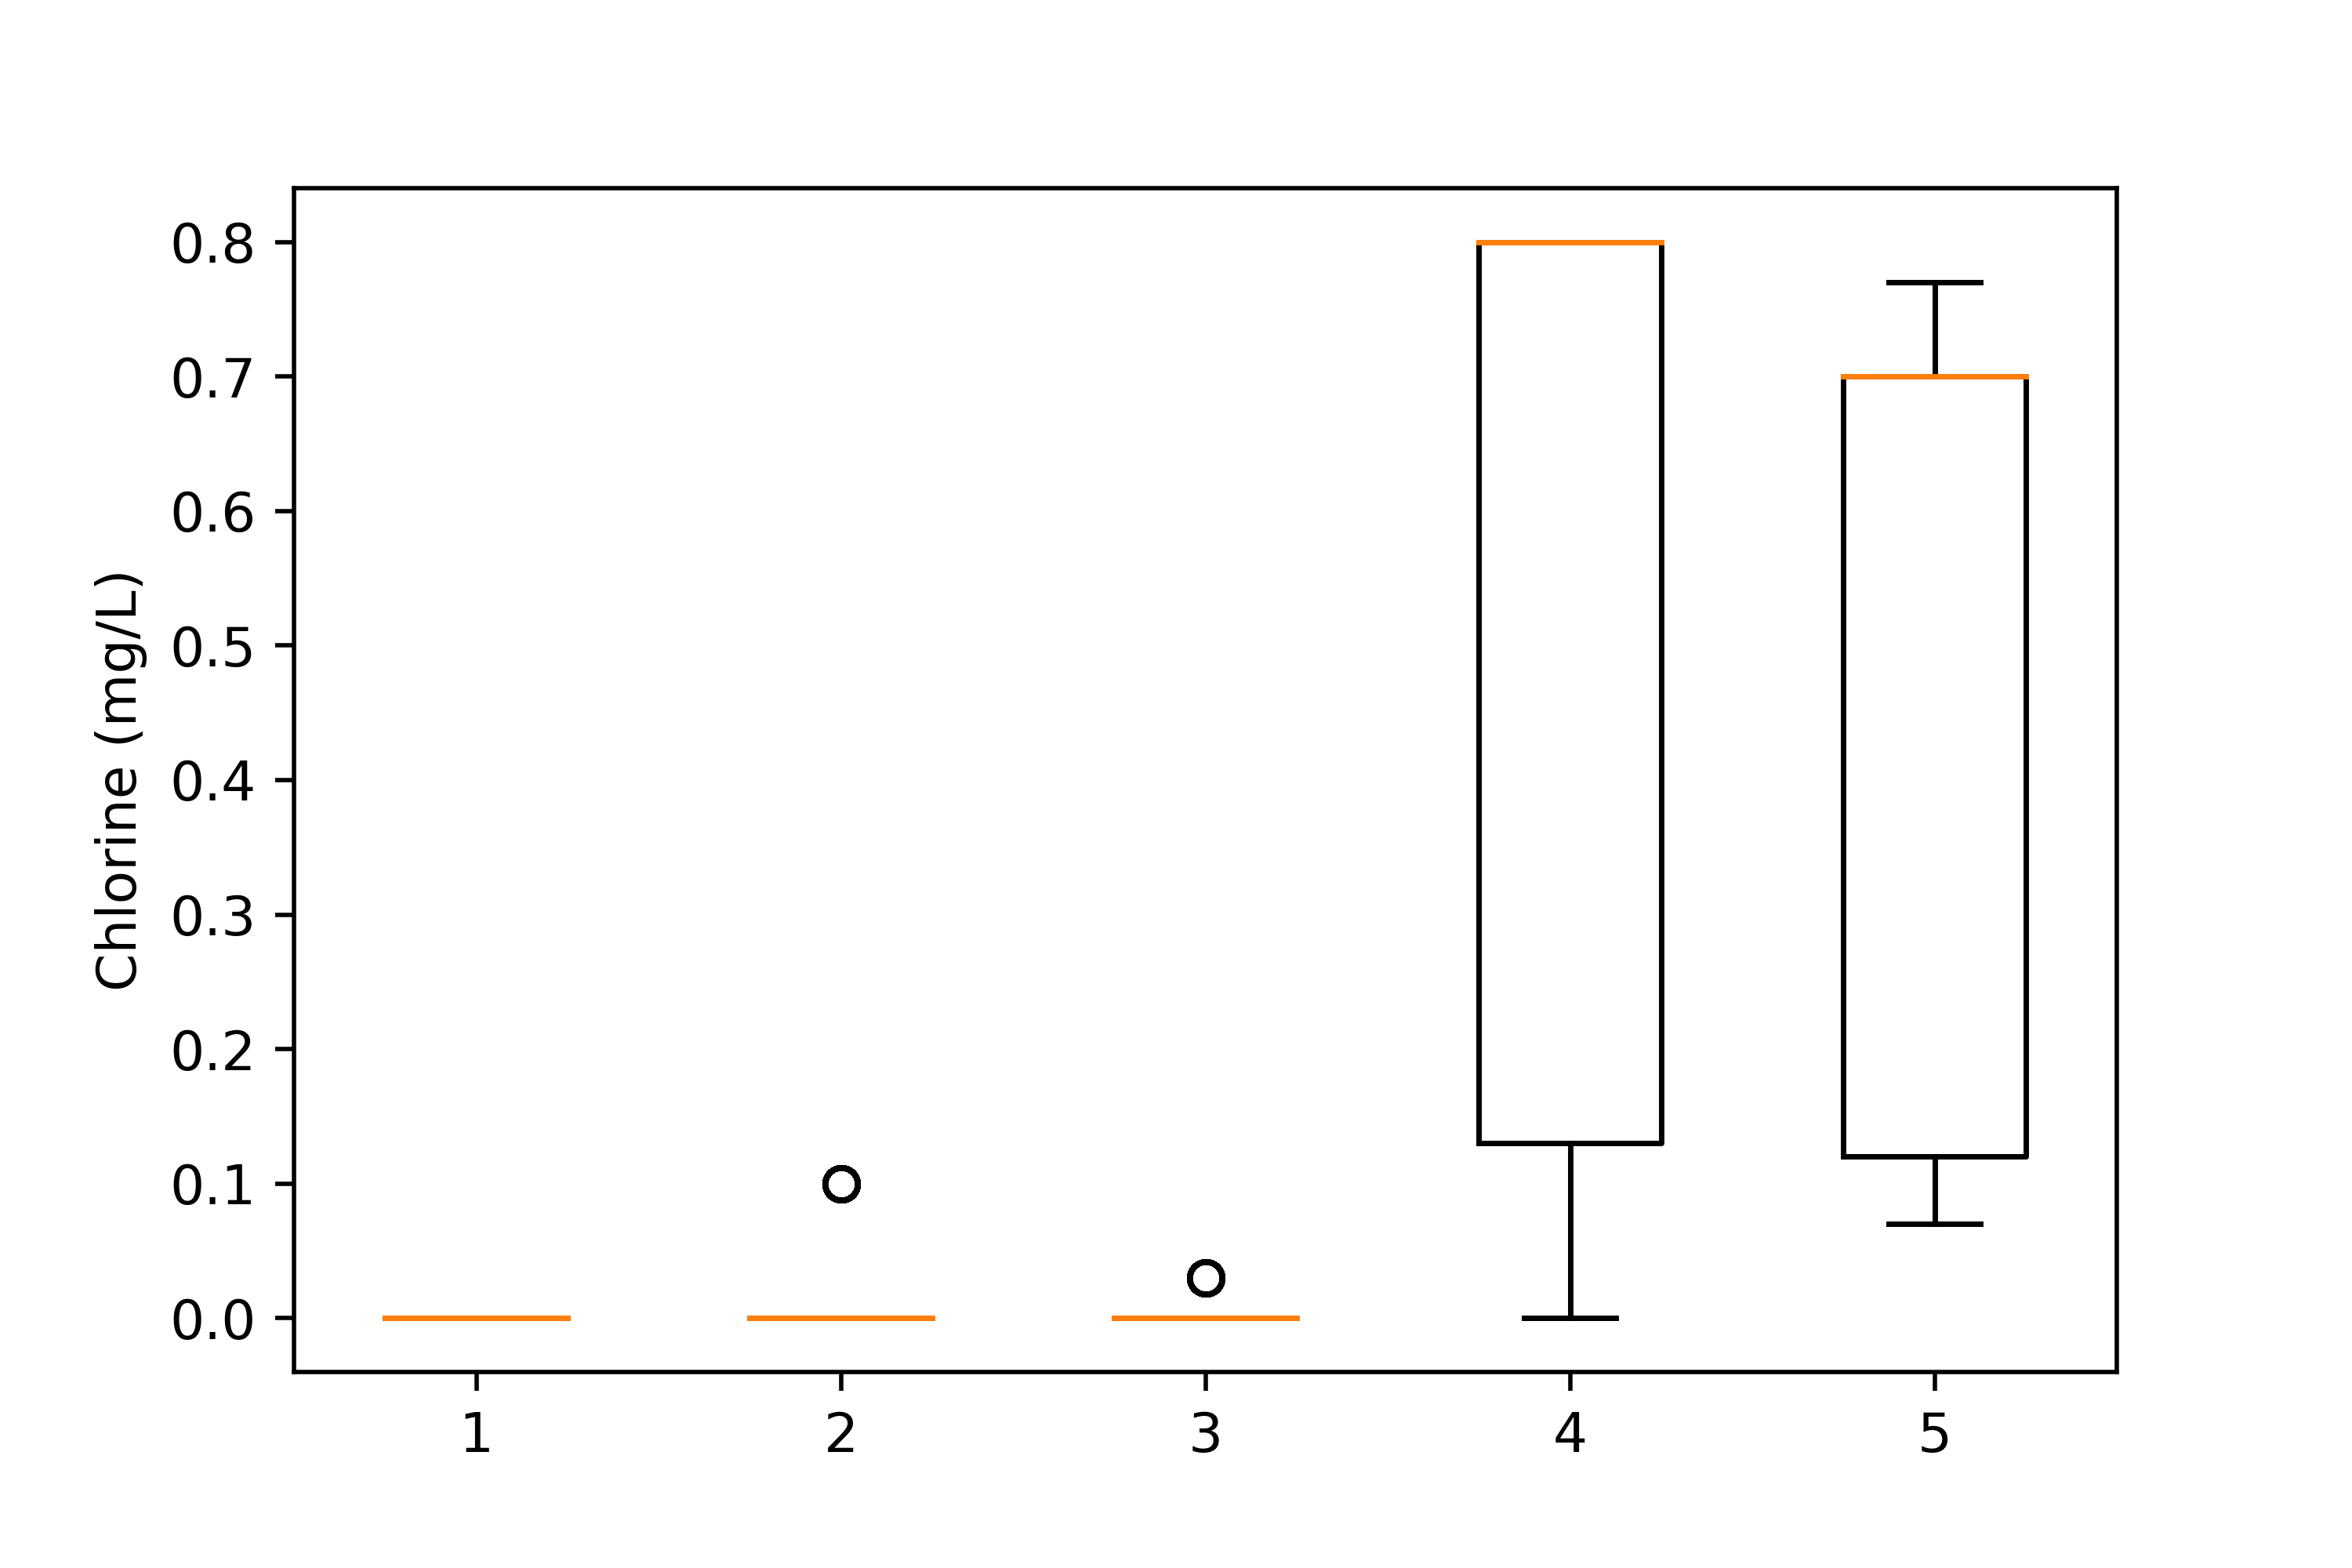
\includegraphics[scale=1.0]{imgss173.png}
	\caption{Diagrama de caja con datos atípicos para cloro residual.}
	\label{fig:figura1000_23}
\end{figure} 

El diagrama de caja para la variable de oxígeno disuelto se muestra en la \autoref{fig:figura1000_24}.

En este caso las gráficas para las diferentes etapas del proceso sí se observan con cambios significativos principalmente a la existencia de múltiples mediciones registradas como datos atípicos en comparación con la tendencia 
dada sin incluir los datos recolectados en el mes de agosto. En el laboratorio de muestreo del OOAPAS se nos mencionó que la posible causa de estos registros era que la alta concentración de contaminantes presentes estaba 
probablemente generando condiciones para las cuales mis sensores no están diseñados, y por lo tanto se tenían valores fuera de la expectativa. Obviamente no se descartó también la posibilidad de que realmente el agua sí 
trajera esos niveles tan elevados de oxígeno disuelto desde la etapa de agua cruda, ya que realmente es muy complicado conocer con exactitud la composición química de los contaminantes que se filtran al agua cruda. 

\clearpage

\begin{figure}[h]
	\centering
	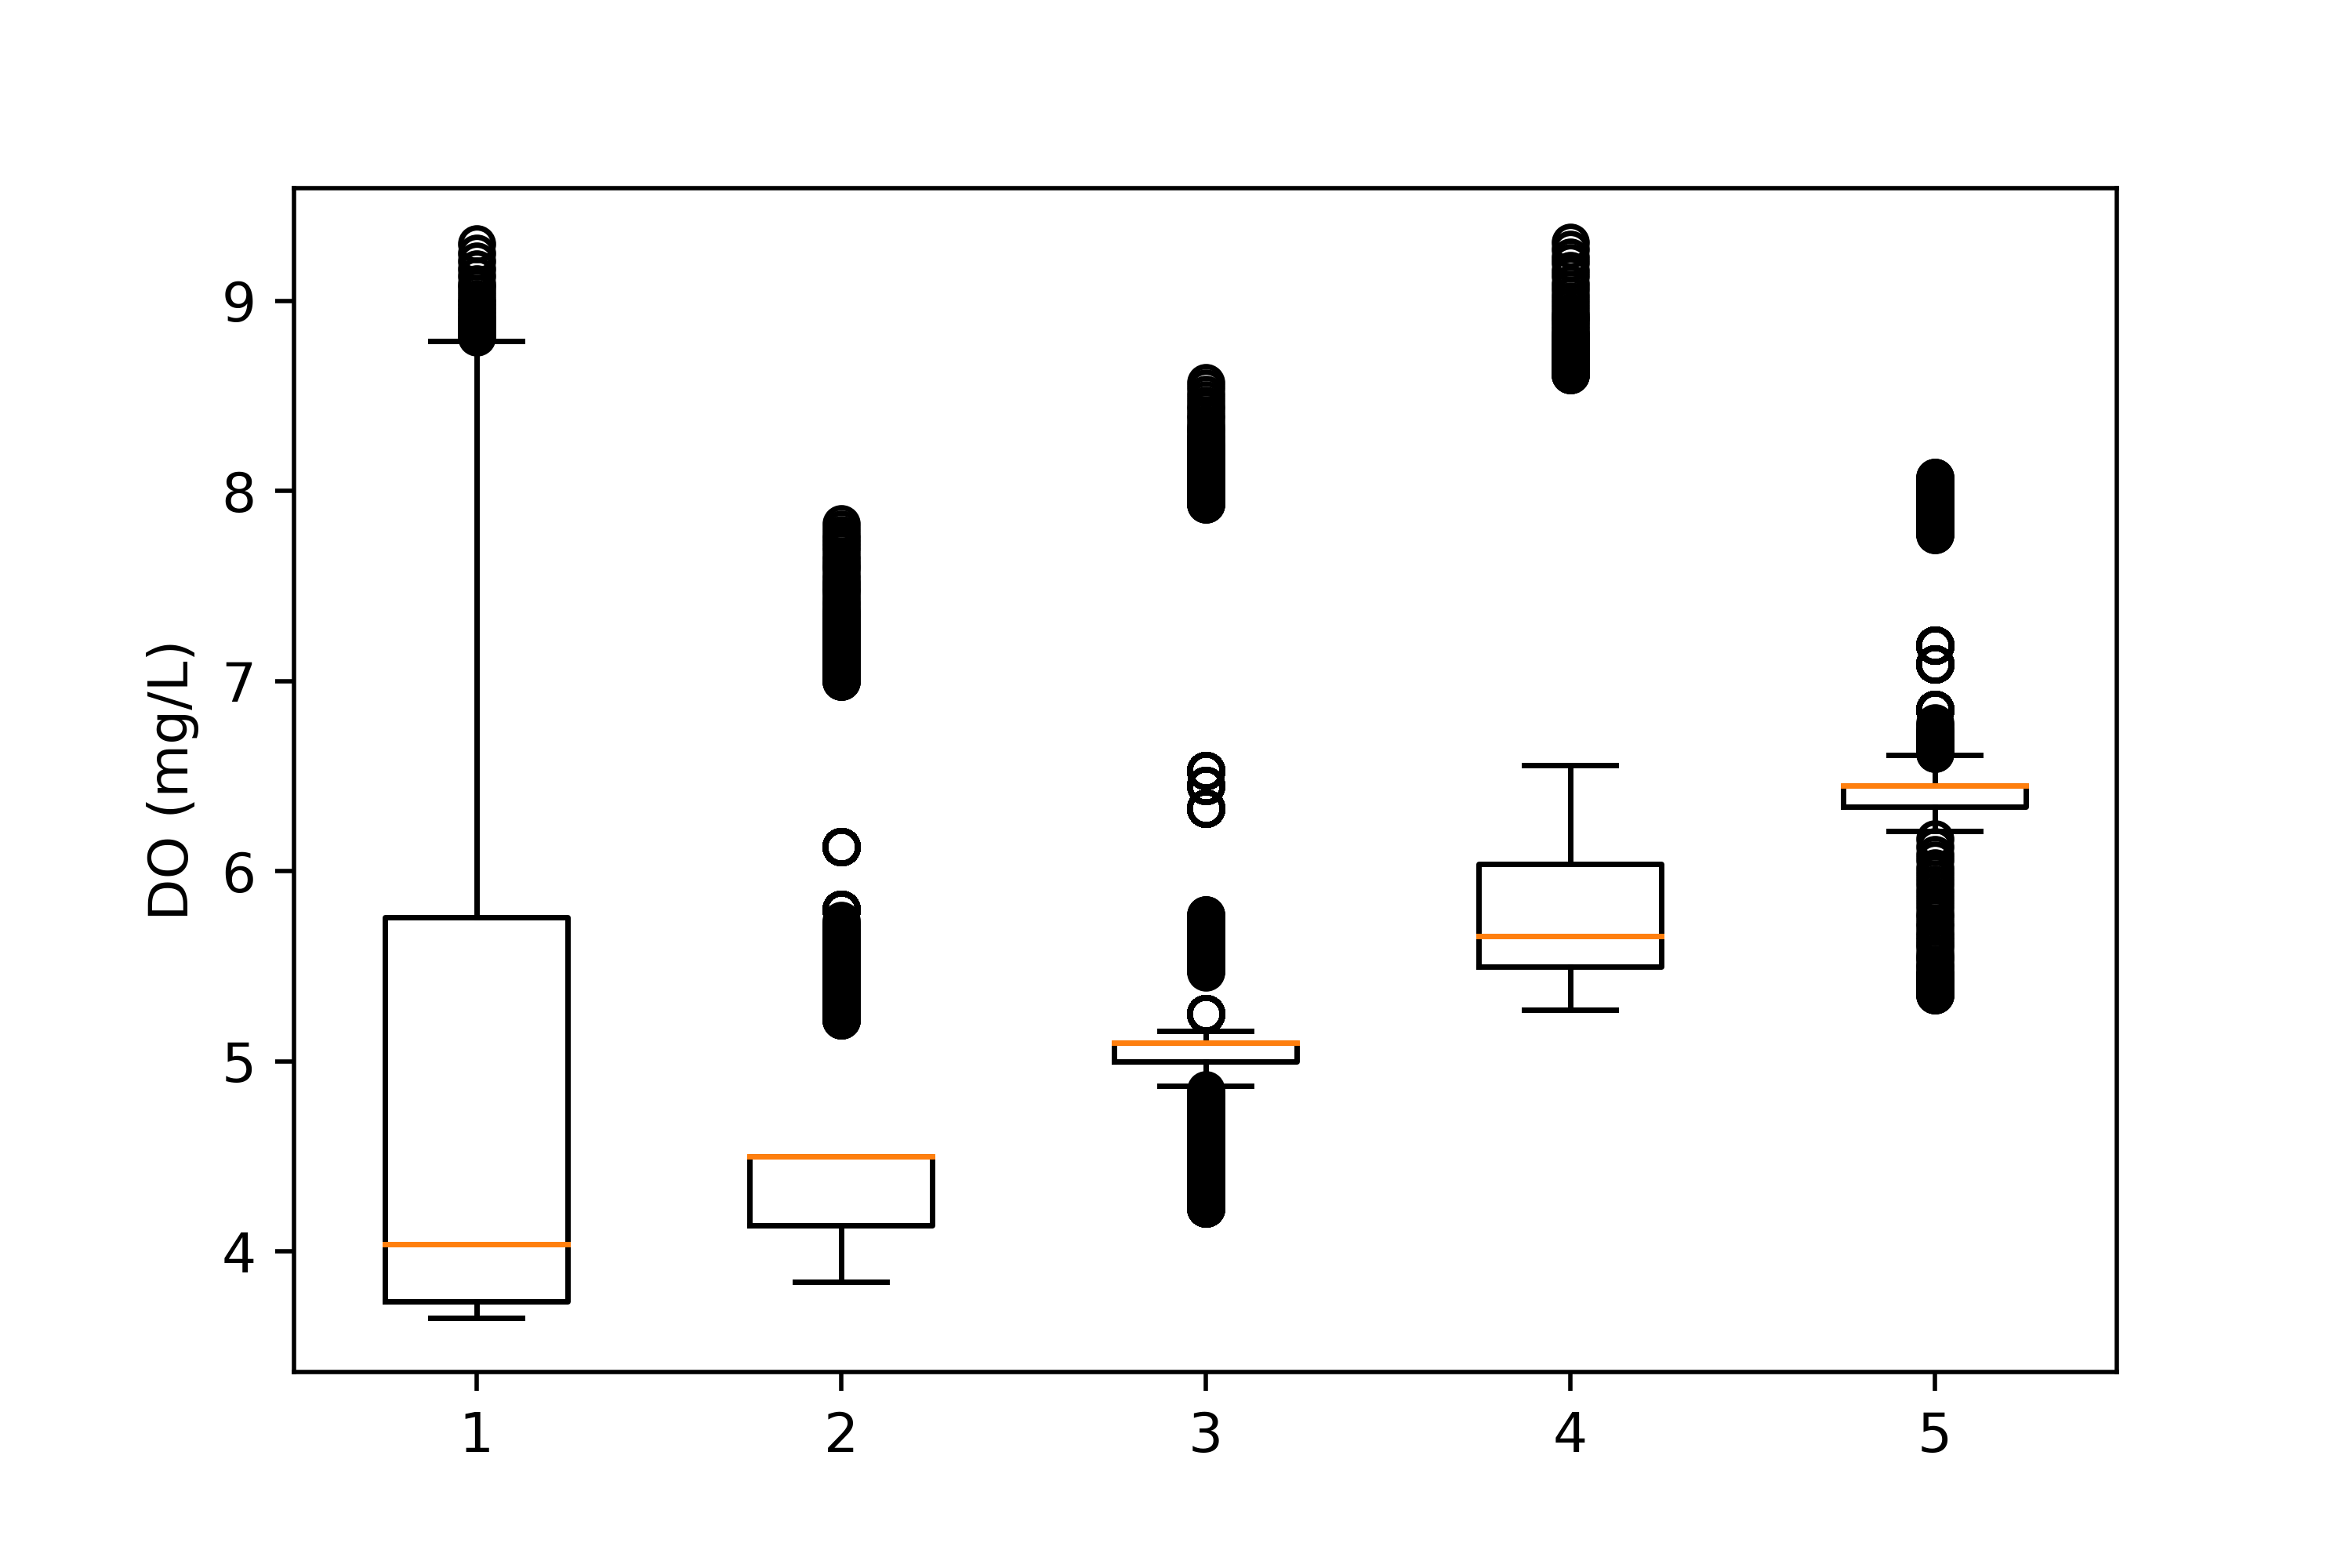
\includegraphics[scale=1.0]{imgss174.png}
	\caption{Diagrama de caja con datos atípicos para oxígeno disuelto.}
	\label{fig:figura1000_24}
\end{figure}

El diagrama de caja para la variable de ORP se muestra en la \autoref{fig:figura1000_25}.

Para la variable de ORP se puede observar que se mantiene la tendencia de un comportamiento incremental al incluir los datos del mes de agosto; para las etapas de salida de filtración y agua potable las gráficas no presentan 
modificaciones, sin embargo en las primeras 3 etapas analizadas sí se tiene la presencia de mediciones atípicas de magnitud elevada en comparación a los resultados sin datos atípicos, además de que los límites superior en 
las gráficas para las etapas de agua cruda y tanque de mezclado rápido se modifican al incluir información del mes de agosto.

\clearpage

\begin{figure}[h]
	\centering
	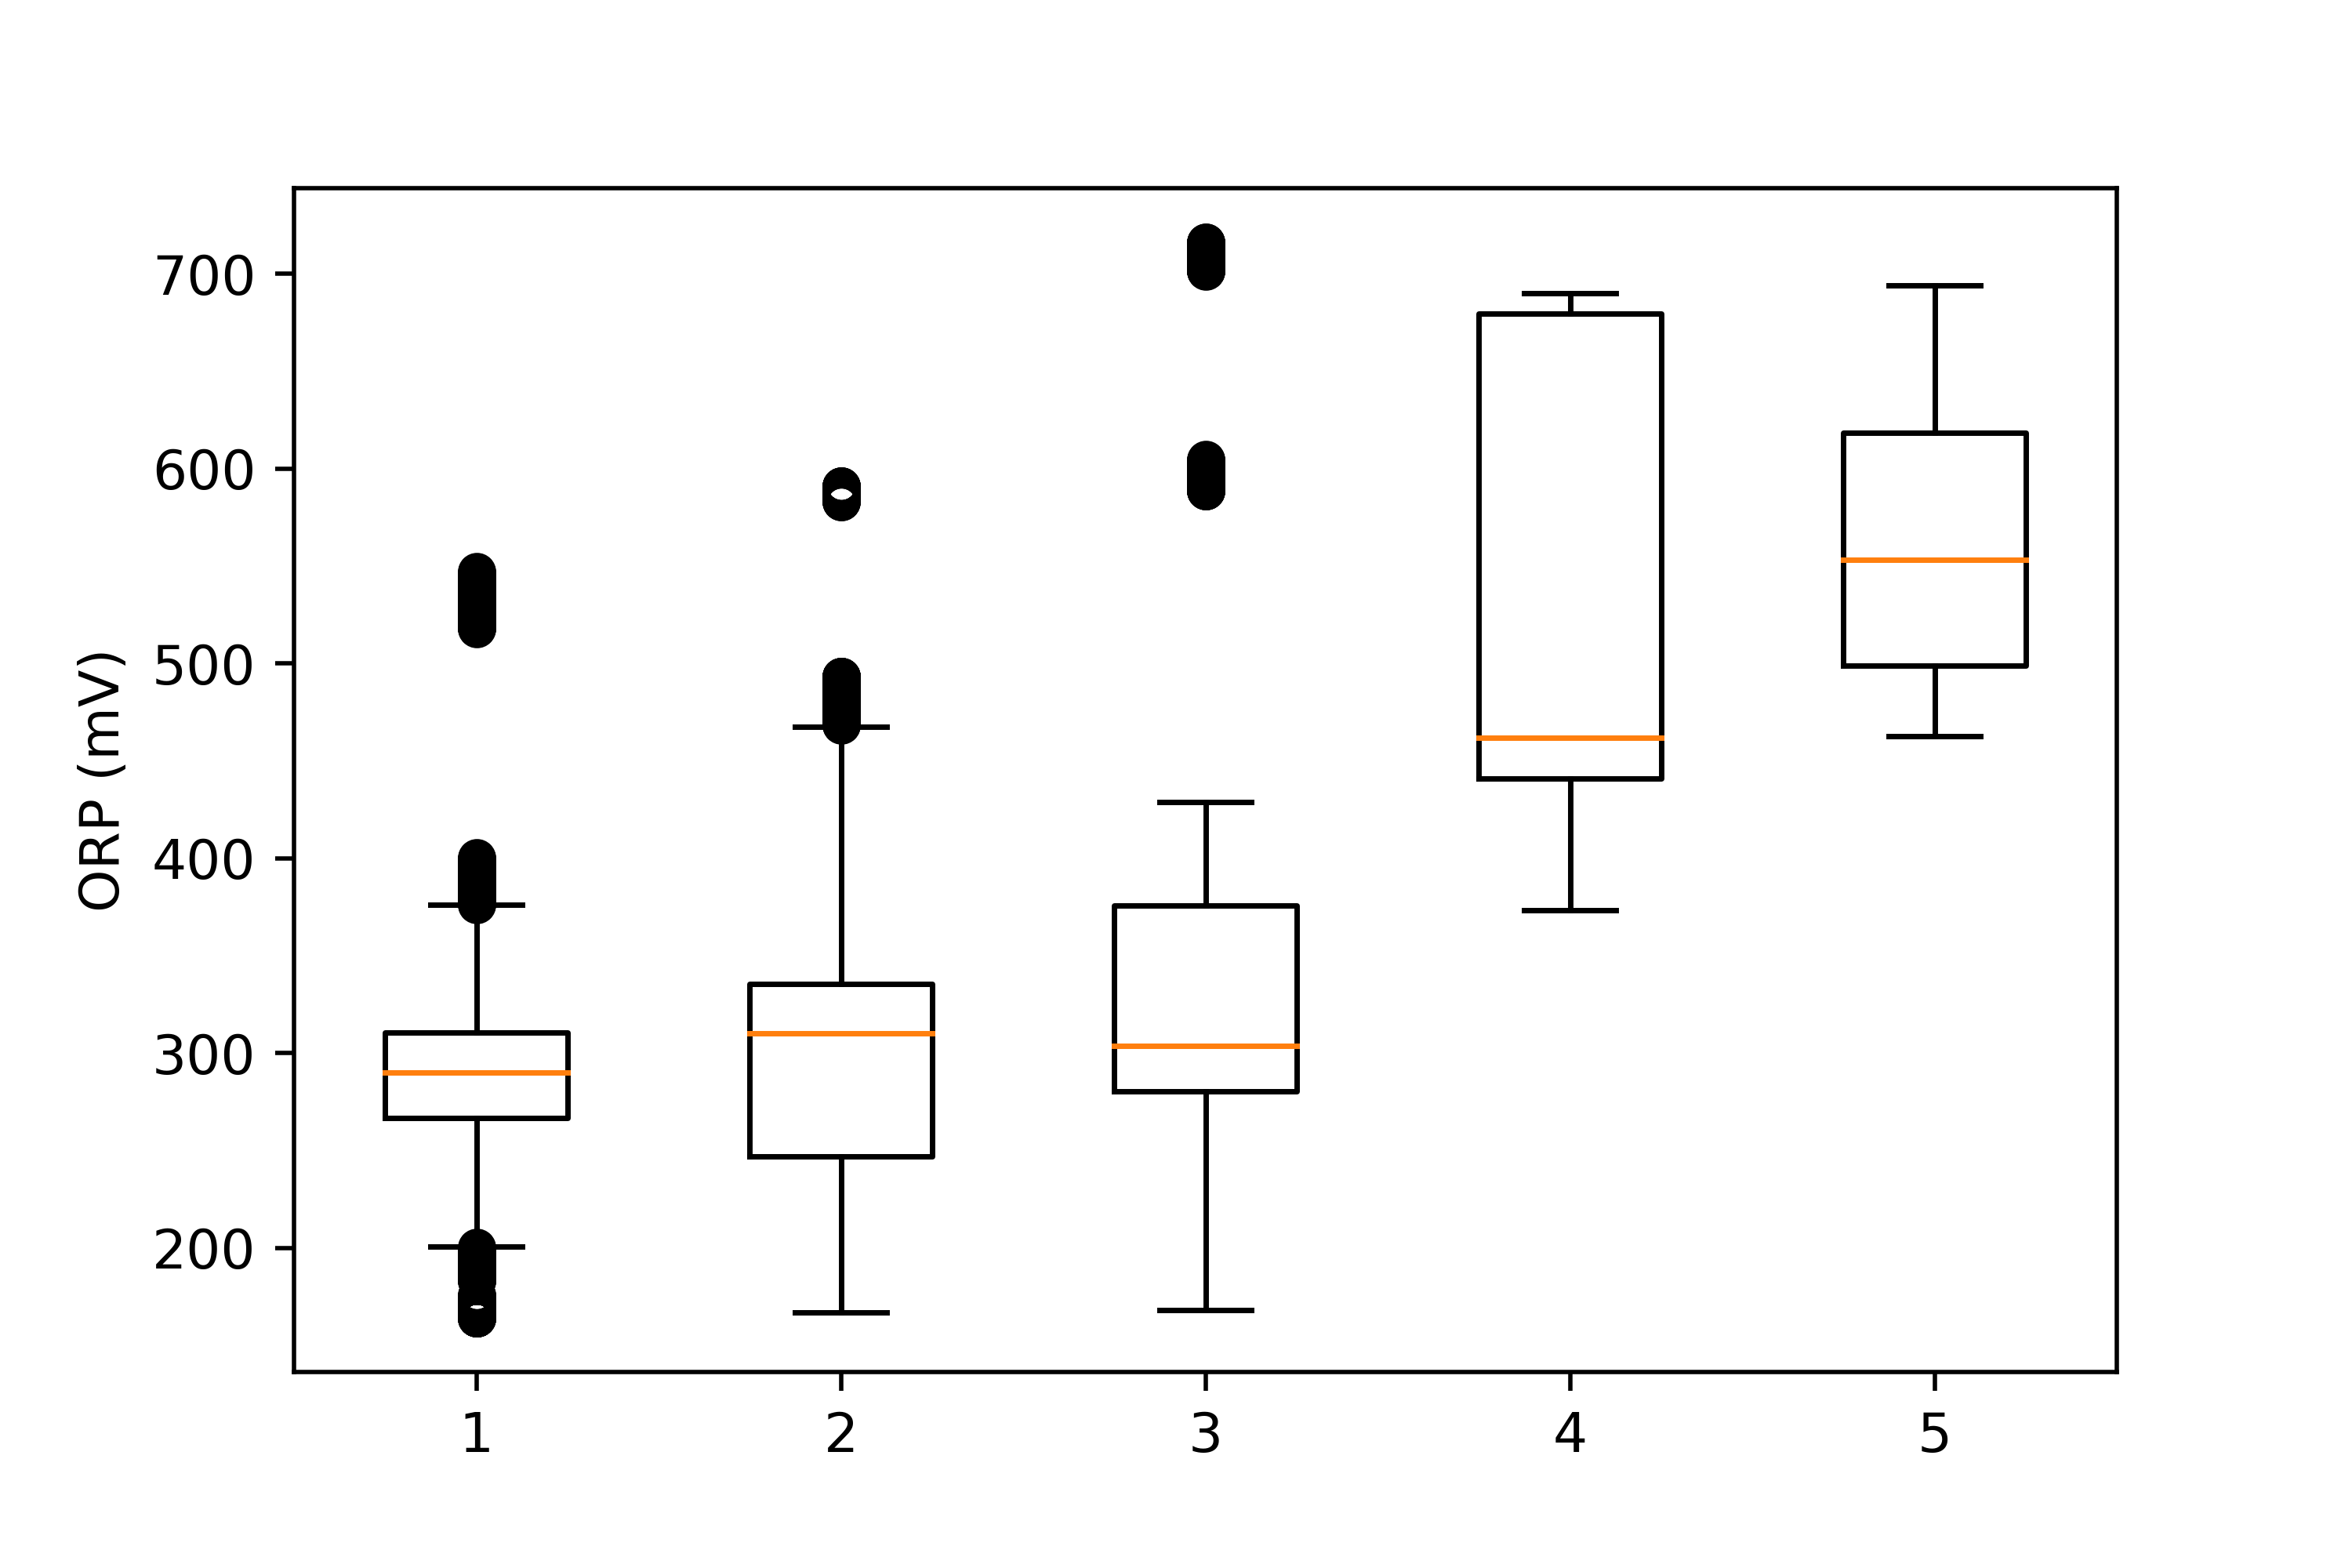
\includegraphics[scale=1.0]{imgss175.png}
	\caption{Diagrama de caja con datos atípicos para ORP.}
	\label{fig:figura1000_25}
\end{figure}

\clearpage

\section{Resultados para modelos de clasificación mediante redes neuronales}

\subsection{Resultados para conjunto principal de datos}

En la \autoref{tab:table200_1} se muestran los resultados más significativos para las pruebas de validación realizadas con el conjunto principal de datos recolectados durante todo el año 2024. Este conjunto de pruebas se 
realizó tomando un 80$\%$ del total de los datos para entrenamiento y el 20$\%$ restante para pruebas de validación.

\begin{table}[h]
	\begin{center}
		\begin{tabular}{| c | c | c | c | c |}
	    	\hline
            Nodos en capas ocultas & Tasa de aprendizaje & Épocas & Función de activación & Aciertos \\ \hline
			5 & 0.25 & 278 & Sigmoide & 94.64\% \\
			5 & 0.25 & 210 & tanh & 95.95\% \\
			8 & 0.25 & 340 & Sigmoide & 93.06\% \\
			8 & 0.25 & 292 & tanh & 97.2\% \\
			10 & 0.25 & 301 & Sigmoide & 95.58\% \\
			10 & 0.25 & 505 & tanh & 98.9\% \\
			15 & 0.25 & 663 & Sigmoide & 99.51\% \\
			15 & 0.25 & 312 & tanh & 98.84\% \\
			20 & 0.25 & 189 & Sigmoide & 94.98\% \\
			20 & 0.25 & 386 & tanh & 99.66\% \\
			25 & 0.25 & 332 & tanh & 99.81\% \\
			30 & 0.25 & 362 & tanh & 97.9\% \\ 
			50 & 0.45 & 201 & tanh & 99.84\% \\
			(20,20) & 0.2 & 114 & tanh & 100\% \\
			(20,20) & 0.3 & 35 & tanh & 98.05\% \\
			(30,30) & 0.2 & 43 & tanh & 99.75\% \\
			(30,30) & 0.3 & 69 & tanh & 100\% \\ \hline
	    \end{tabular}	
		\caption{Resultados de validación de la red neuronal para conjunto principal de datos.}
        \label{tab:table200_1}	
	\end{center}
\end{table}

La validación consistió en iniciar probando redes neuronales pequeñas con 1 sola capa oculta y pocos nodos en ella, y se fue incrementando el número de nodos de forma gradual; finalmente se hicieron pruebas con redes de 
2 capas ocultas con casos de 20 y 30 nodos en cada una de las capas. Adicionalmente, al ir ejecutando las pruebas se iba intercambiando la función de activación en las capas ocultas entre la función sigmoide y la función 
tangente hiperbólica para tener la comparativa y tener evidencia para obtener conclusiones sobre qué función de activación tiene mejor rendimiento para esta aplicación en específico.

A continuación se muestran resultados representativos de las curvas de entrenamiento donde se muestra el comportamiento de la función de error para pruebas incluidas en la \autoref{tab:table200_1}. 

\clearpage

\begin{figure}[h]
	\centering
	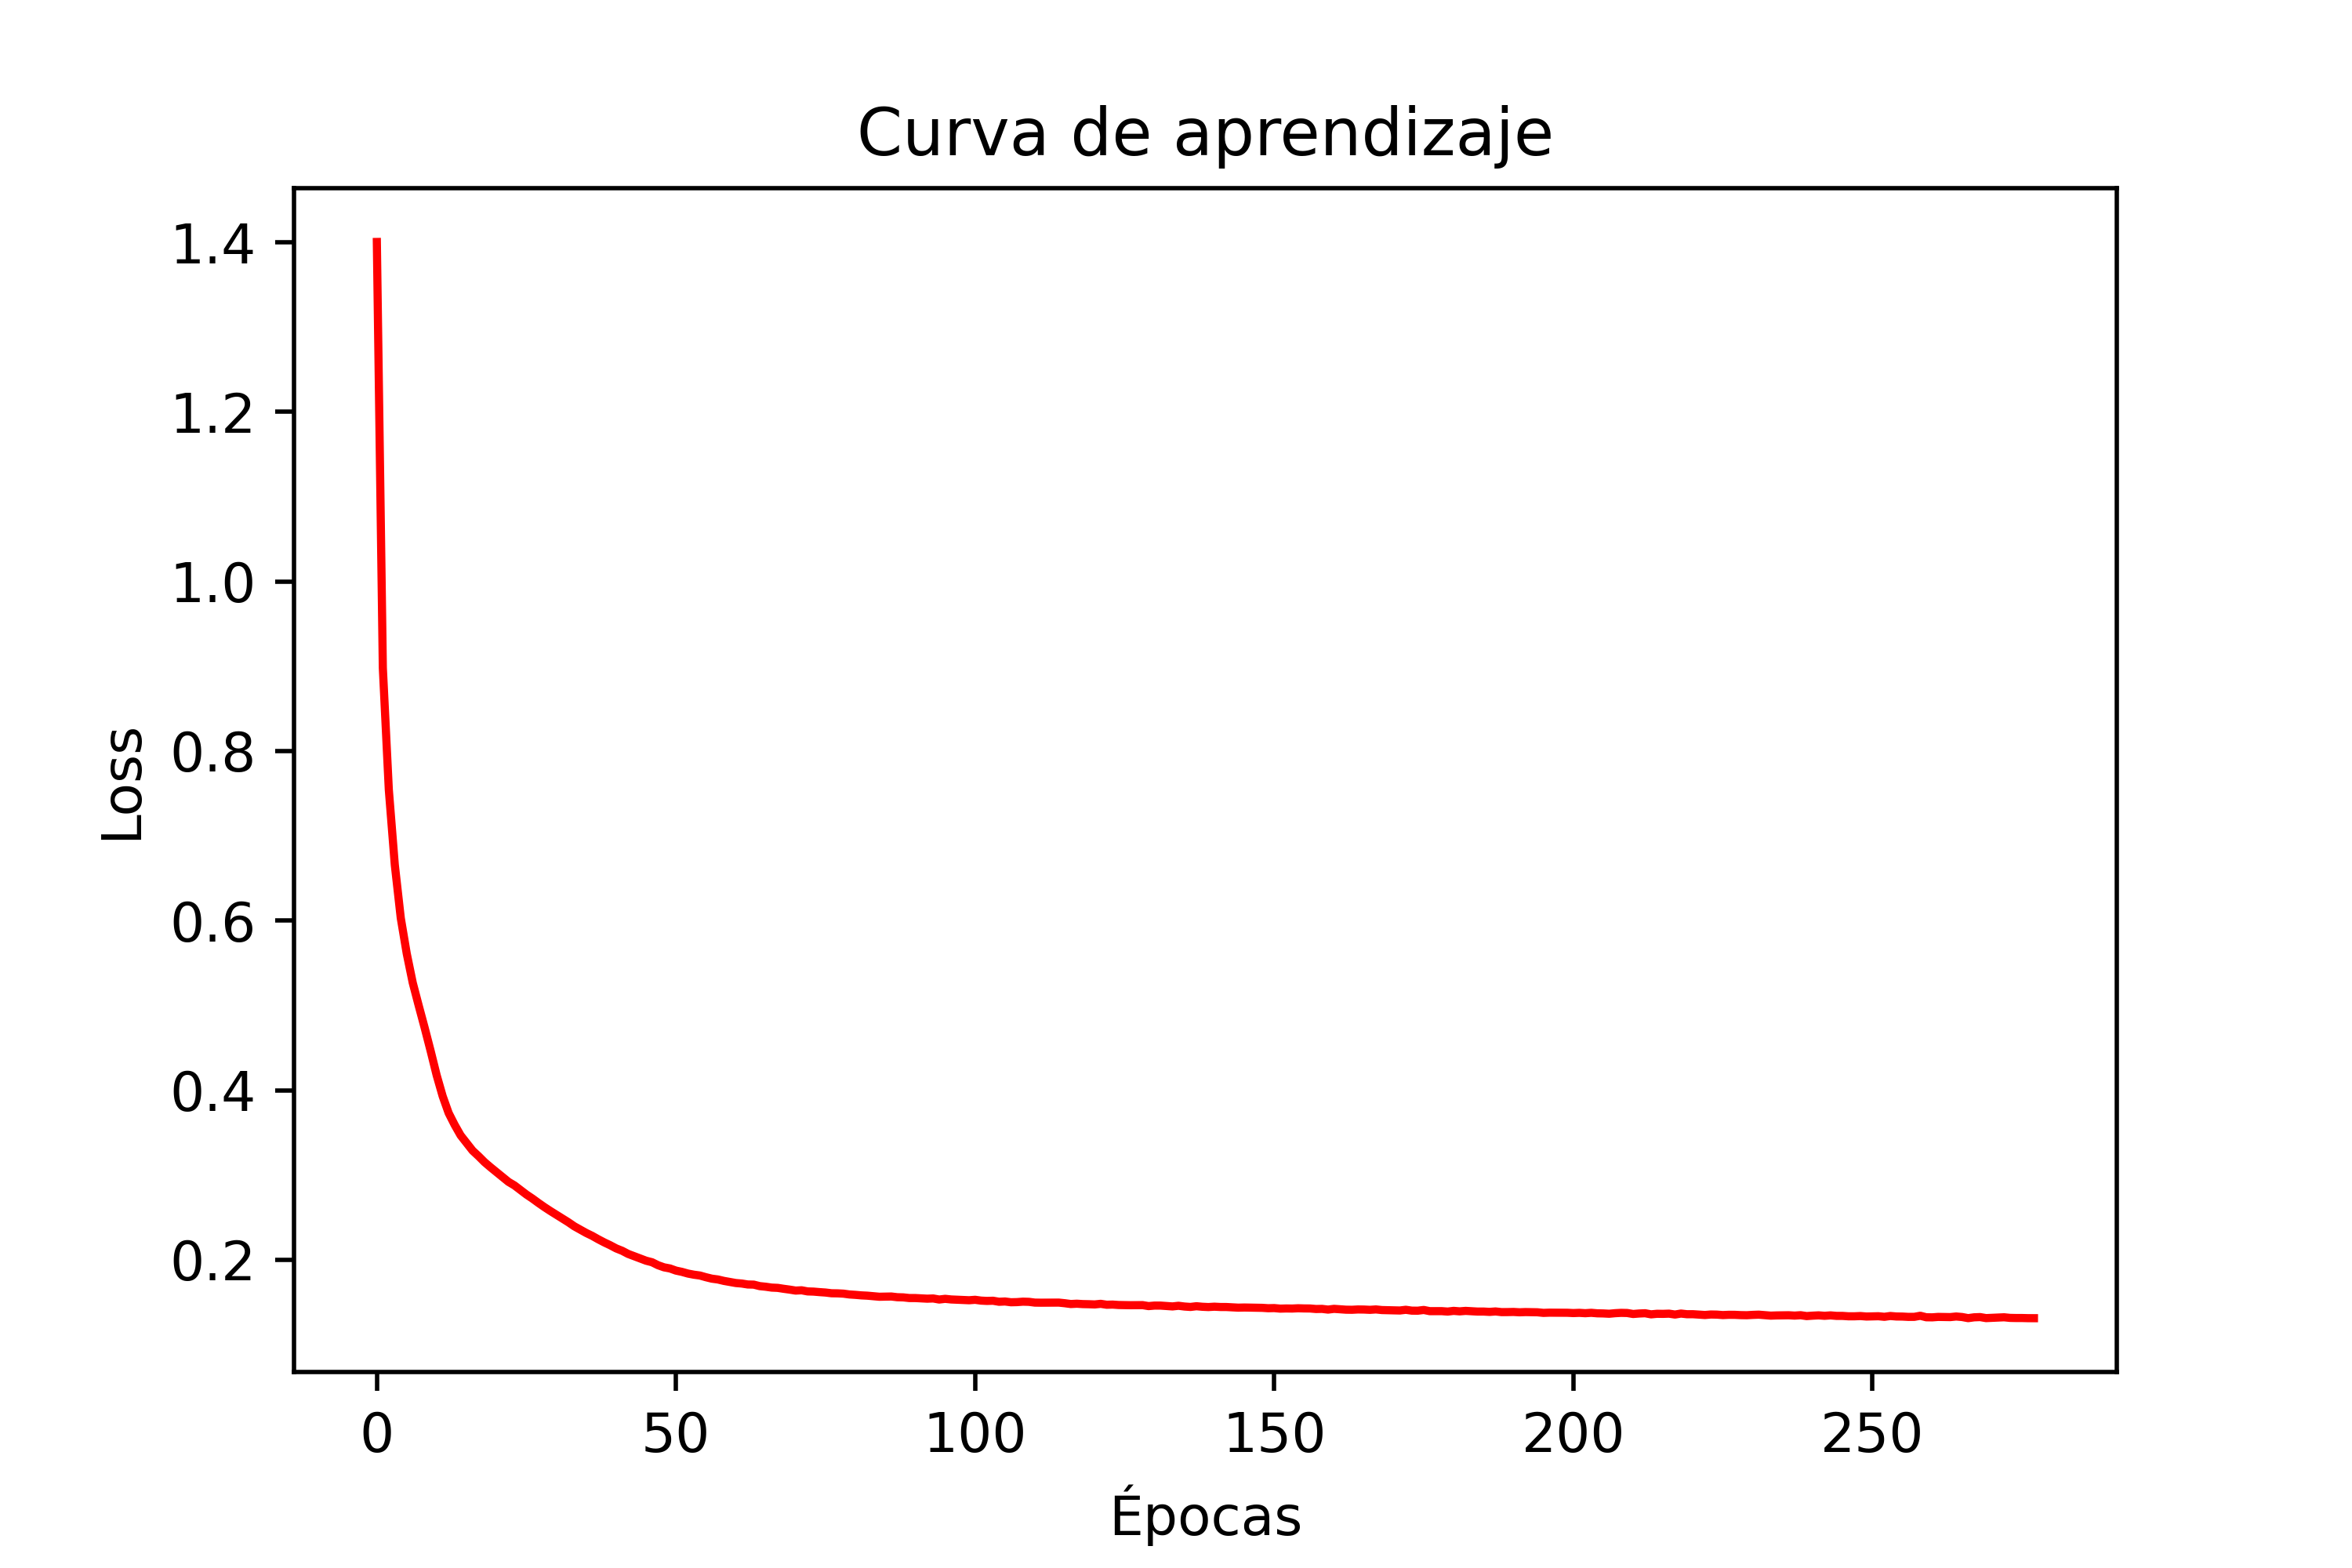
\includegraphics[scale=0.71]{imgss176.png}
	\caption{Resultado 1}
	\label{fig:figura1000_26}
\end{figure}

El resultado de la \autoref{fig:figura1000_26} corresponde a una red neuronal con 1 capa oculta, 5 nodos en ella y un valor de 0.25 como tasa de aprendizaje. La función de activación utilizada para las capas ocultas es la 
función sigmoide y logra un porcentaje de aciertos de 94.64$\%$ después de ejecutar 278 épocas de entrenamiento. En este caso, el proceso de minimización del error alcanzó un valor estable aproximadamente al alcanzar 
150 épocas de entrenamiento, hasta el punto de llegar a 278 épocas donde el algoritmo converge al alcanzar el valor más pequeño posible.

\begin{figure}[h]
	\centering
	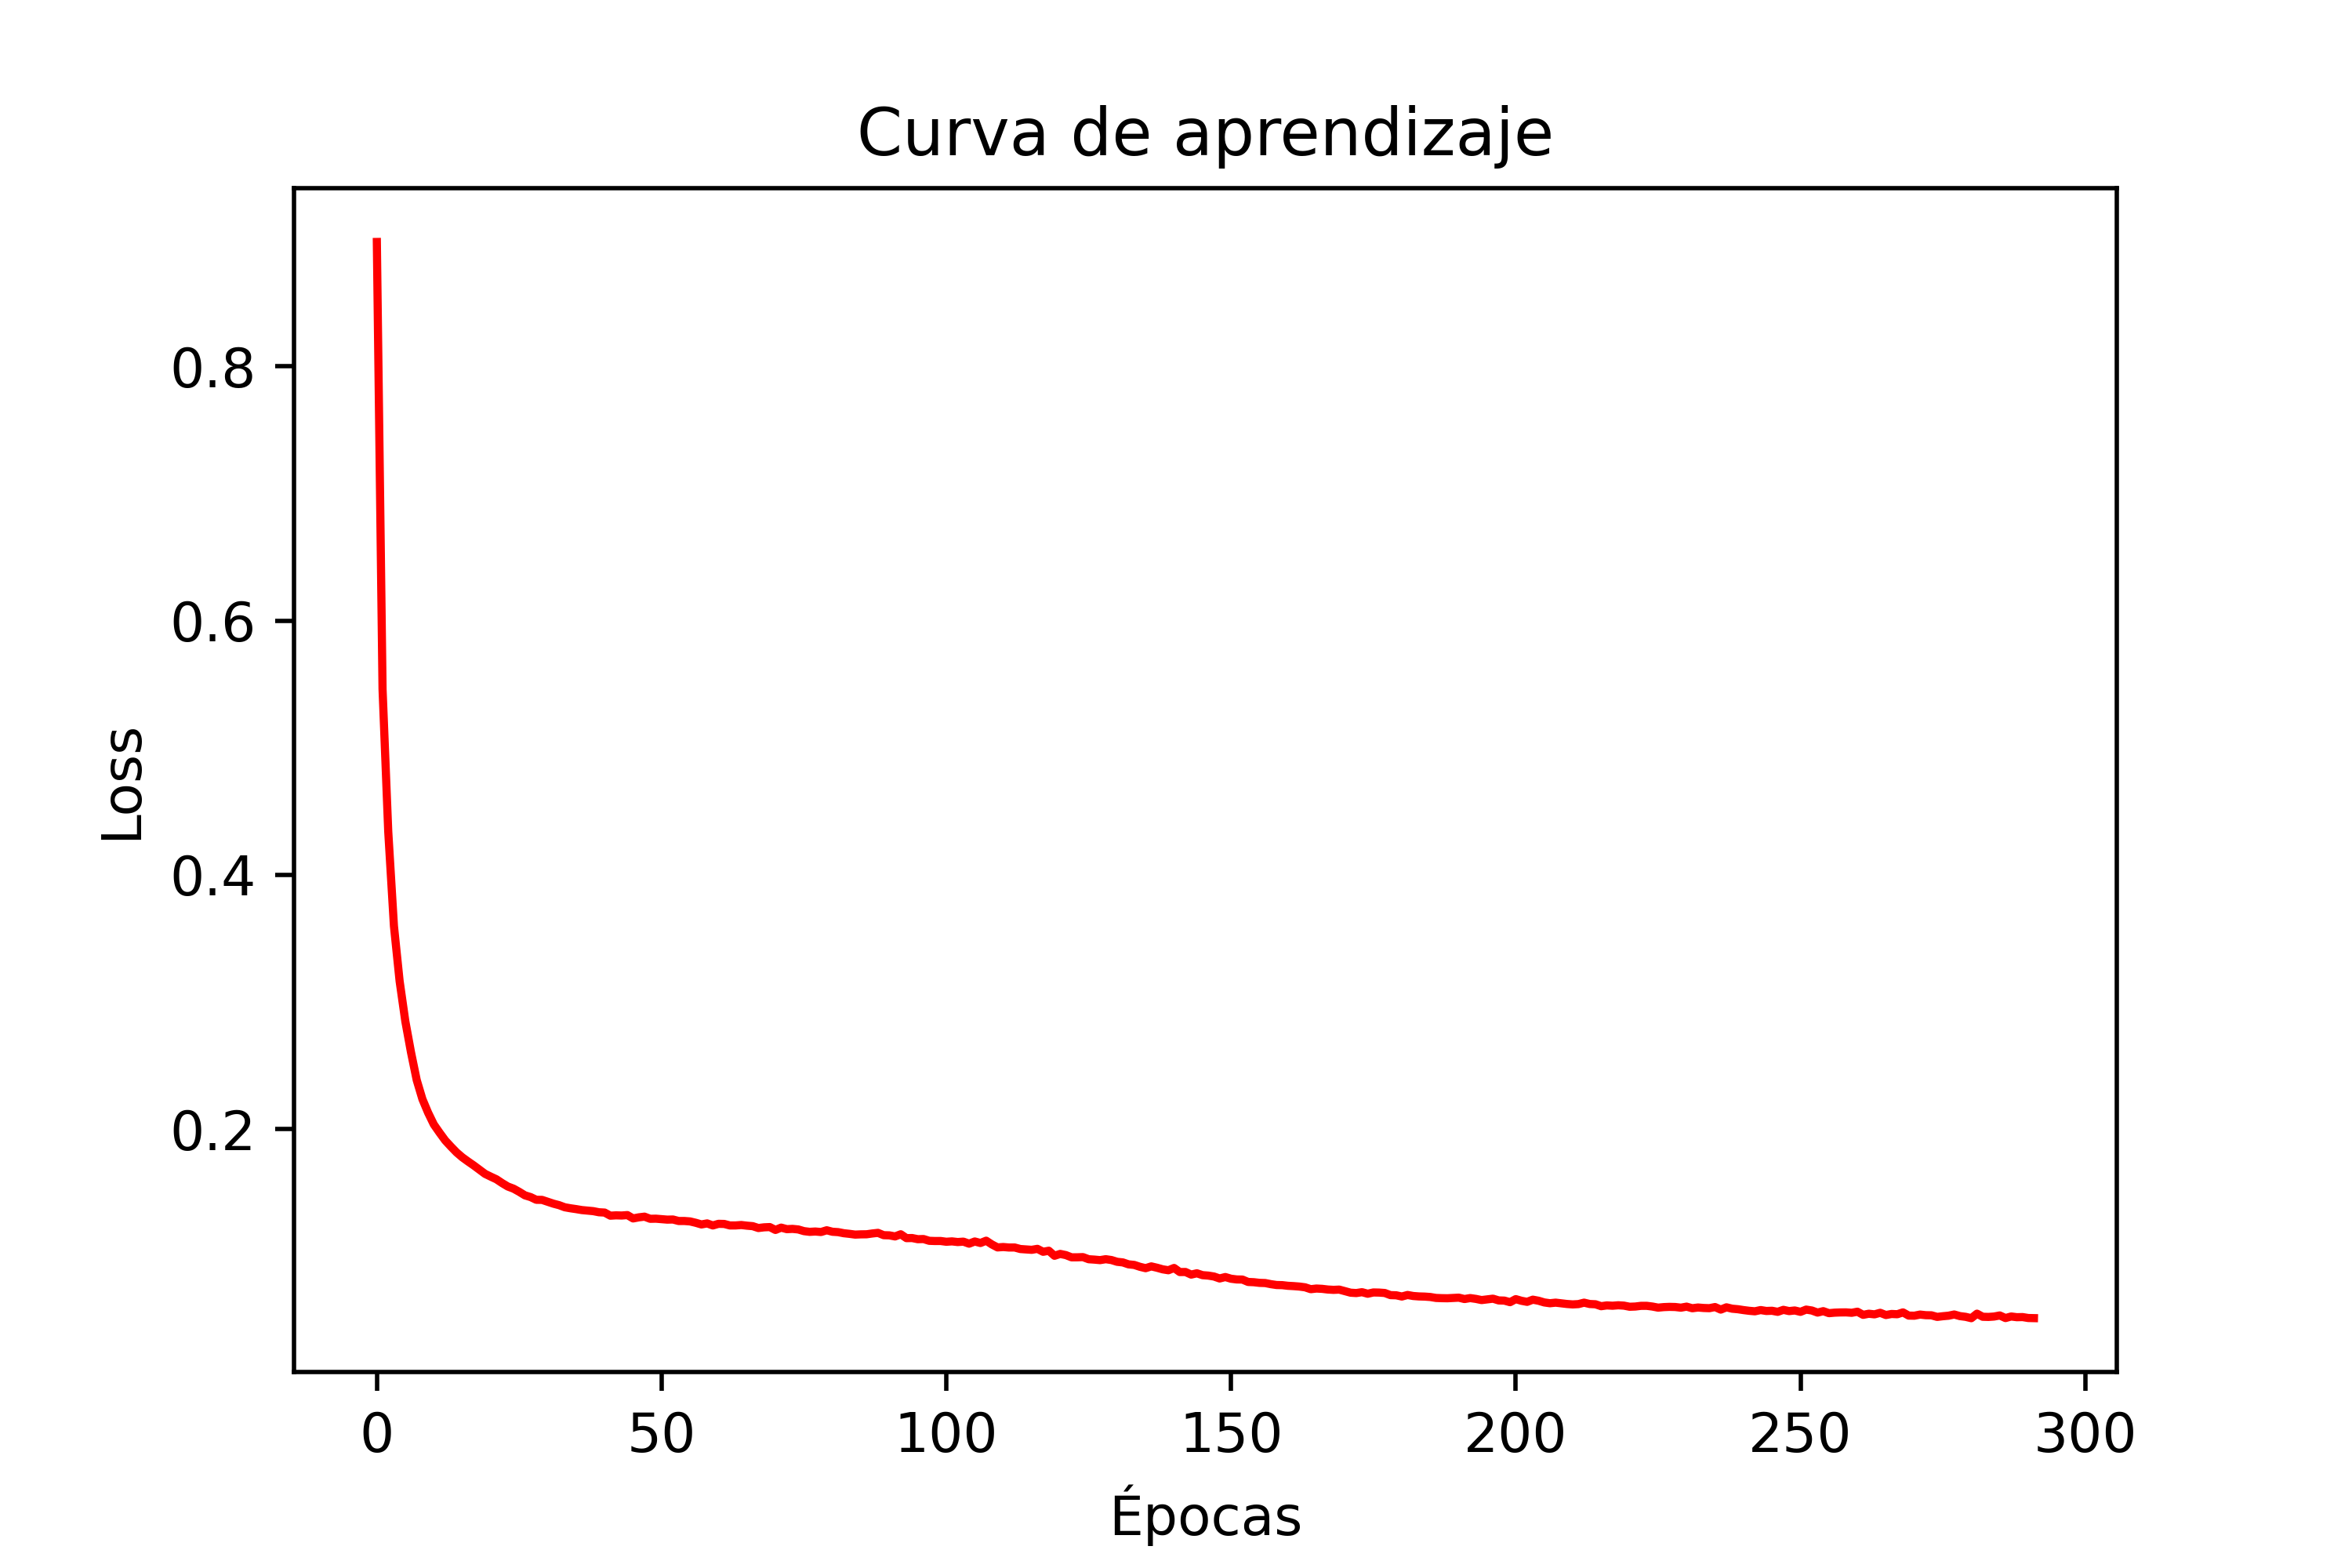
\includegraphics[scale=0.71]{imgss179.png}
	\caption{Resultado 4.}
	\label{fig:figura1000_29}
\end{figure} 

El resultado de la \autoref{fig:figura1000_29} corresponde a una red neuronal con 1 capa oculta, 8 nodos en ella y un valor de 0.25 como tasa de aprendizaje. La función de activación utilizada para las capas ocultas es la 
función tangente hiperbólica y logra un porcentaje de aciertos de 97.2$\%$ después de ejecutar 292 épocas de entrenamiento. En este caso, el proceso de minimización del error alcanzó un valor estable después de 150 épocas 
de entrenamiento hasta converger en 292 épocas sin lograr un valor de 0 para la función de error.

\begin{figure}[h]
	\centering
	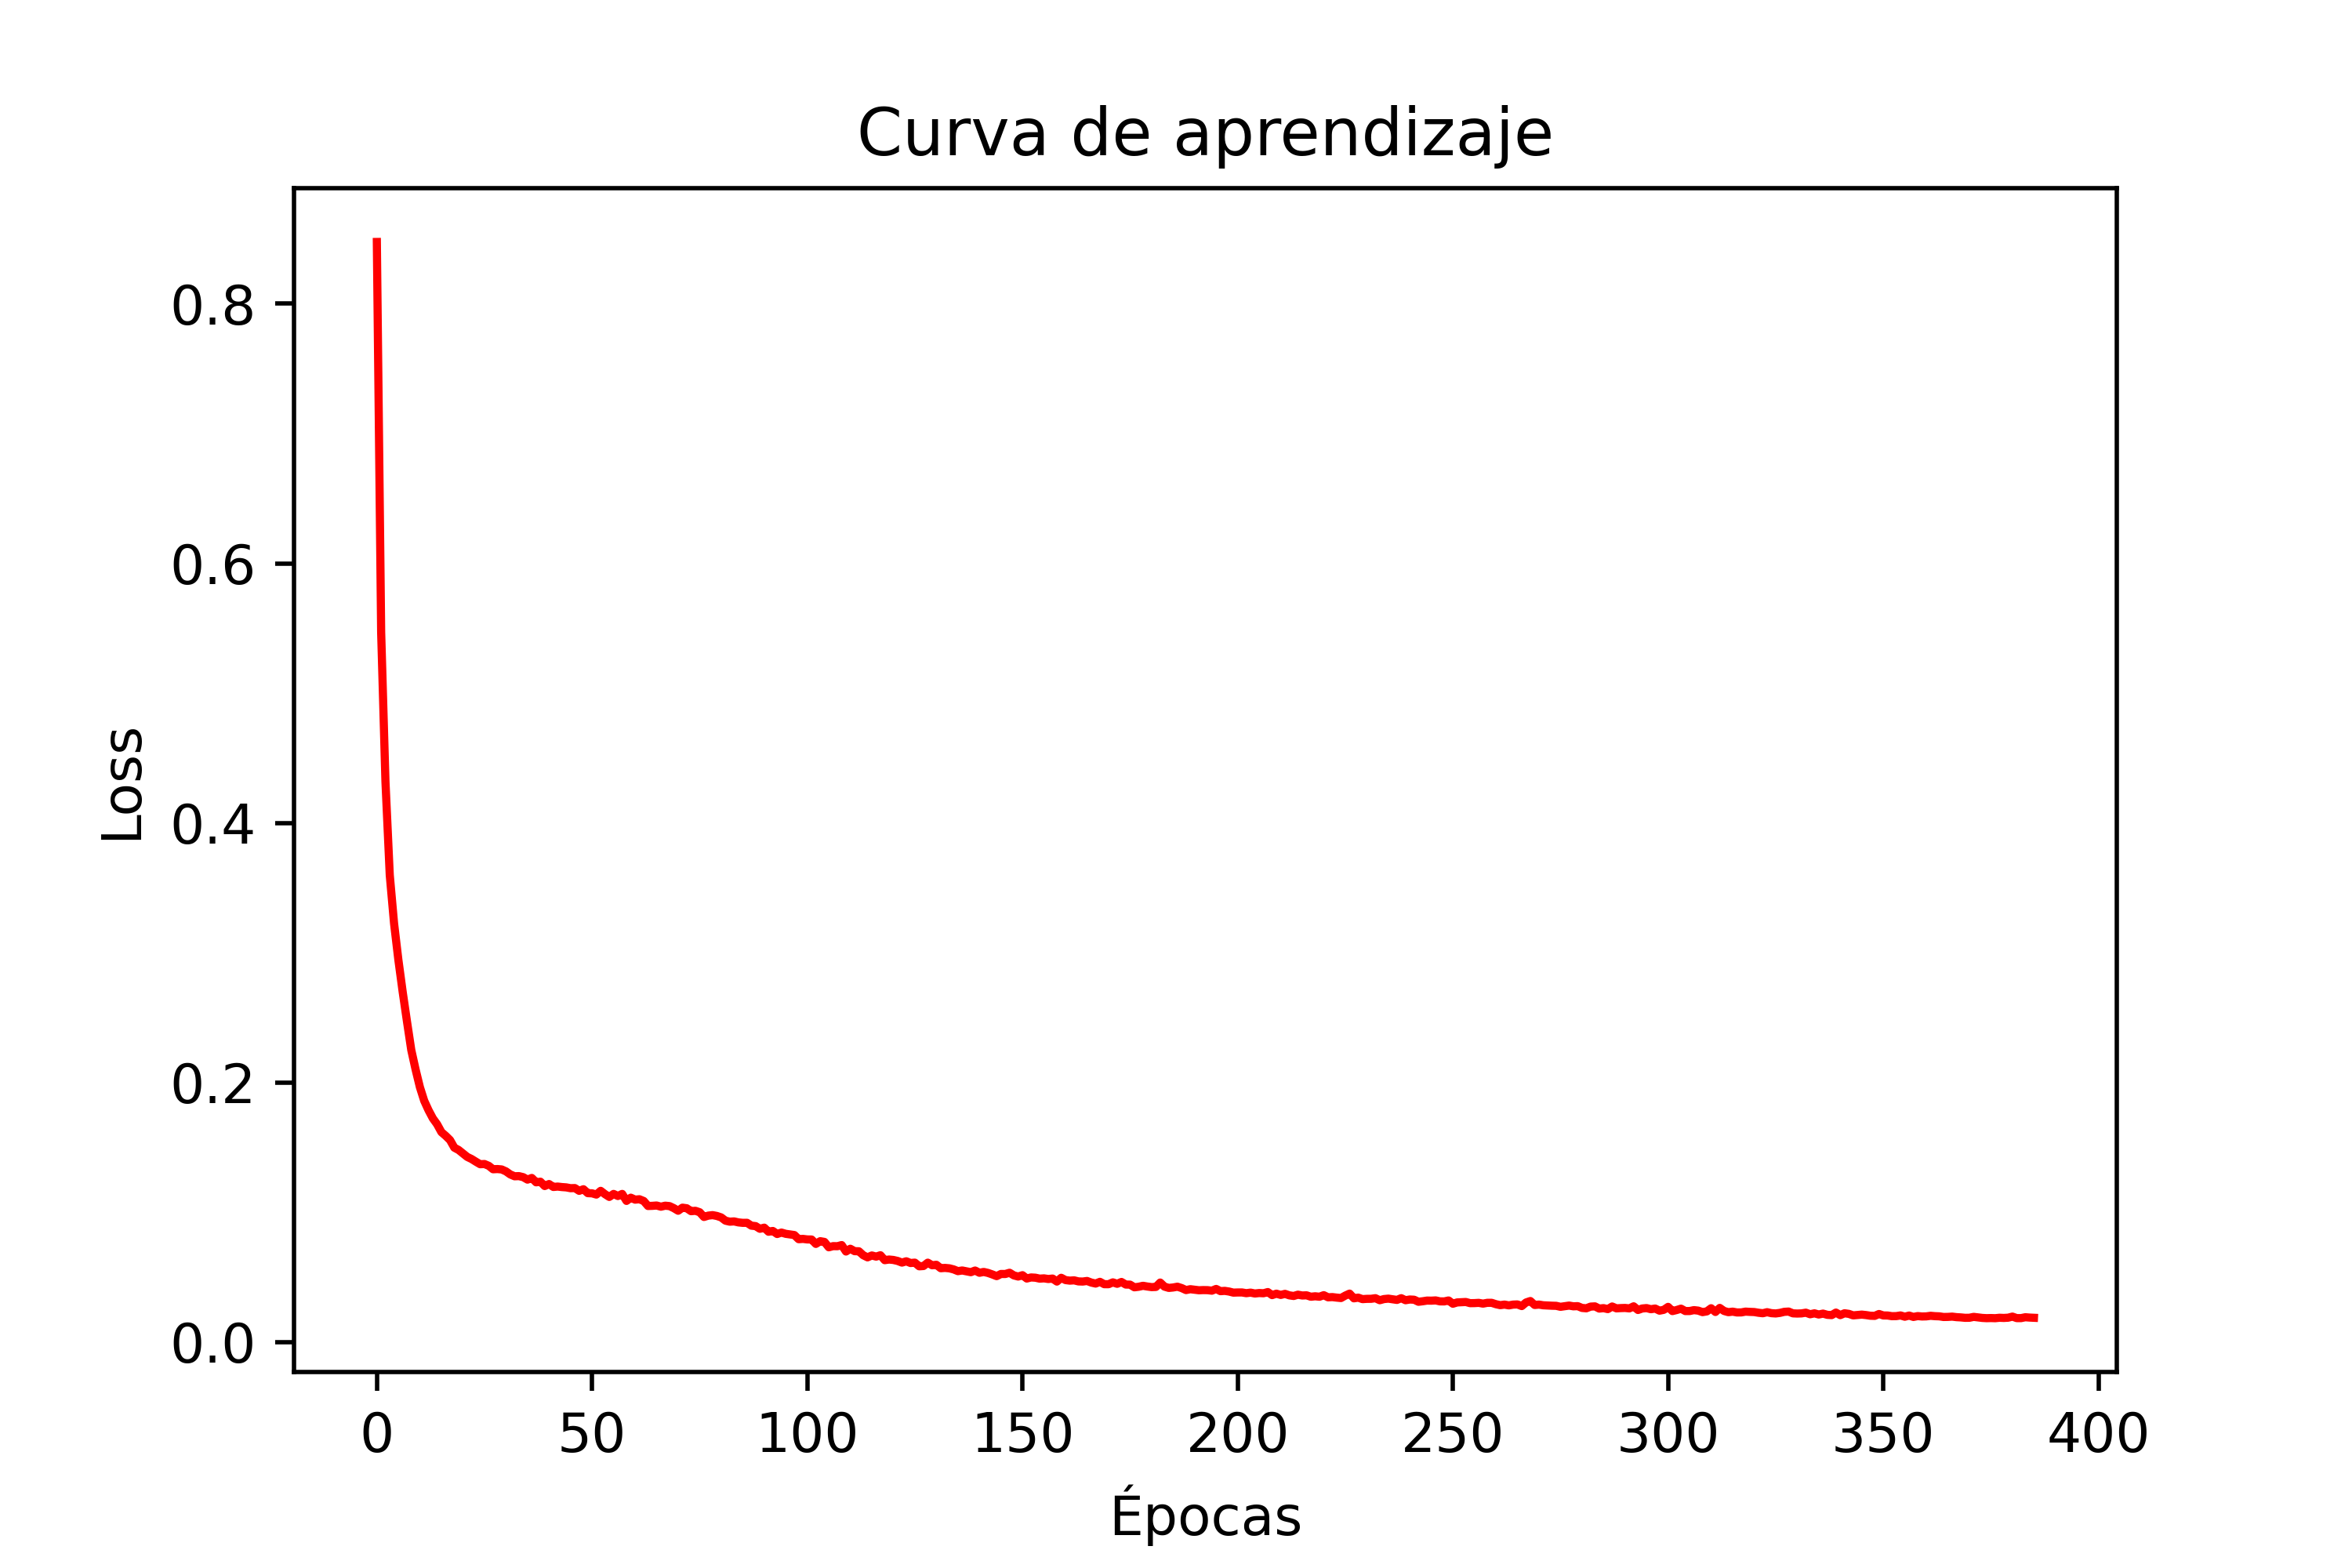
\includegraphics[scale=0.71]{imgss185.png}
	\caption{Resultado 10.}
	\label{fig:figura1000_35}
\end{figure}

El resultado de la \autoref{fig:figura1000_35} corresponde a una red neuronal con 1 capa oculta, 20 nodos en ella y un valor de 0.25 como tasa de aprendizaje. La función de activación para las capas ocultas es la 
función tangente hiperbólica y logra un porcentaje de aciertos de 99.66$\%$ después de ejecutar 386 épocas de entrenamiento. La minimización del error alcanza un valor estable aproximadamente al llegar a 250 épocas de 
entrenamiento hasta converger en 386 épocas, sin lograr alcanzar un valor de 0 para fase de entrenamiento.

\begin{figure}[h]
	\centering
	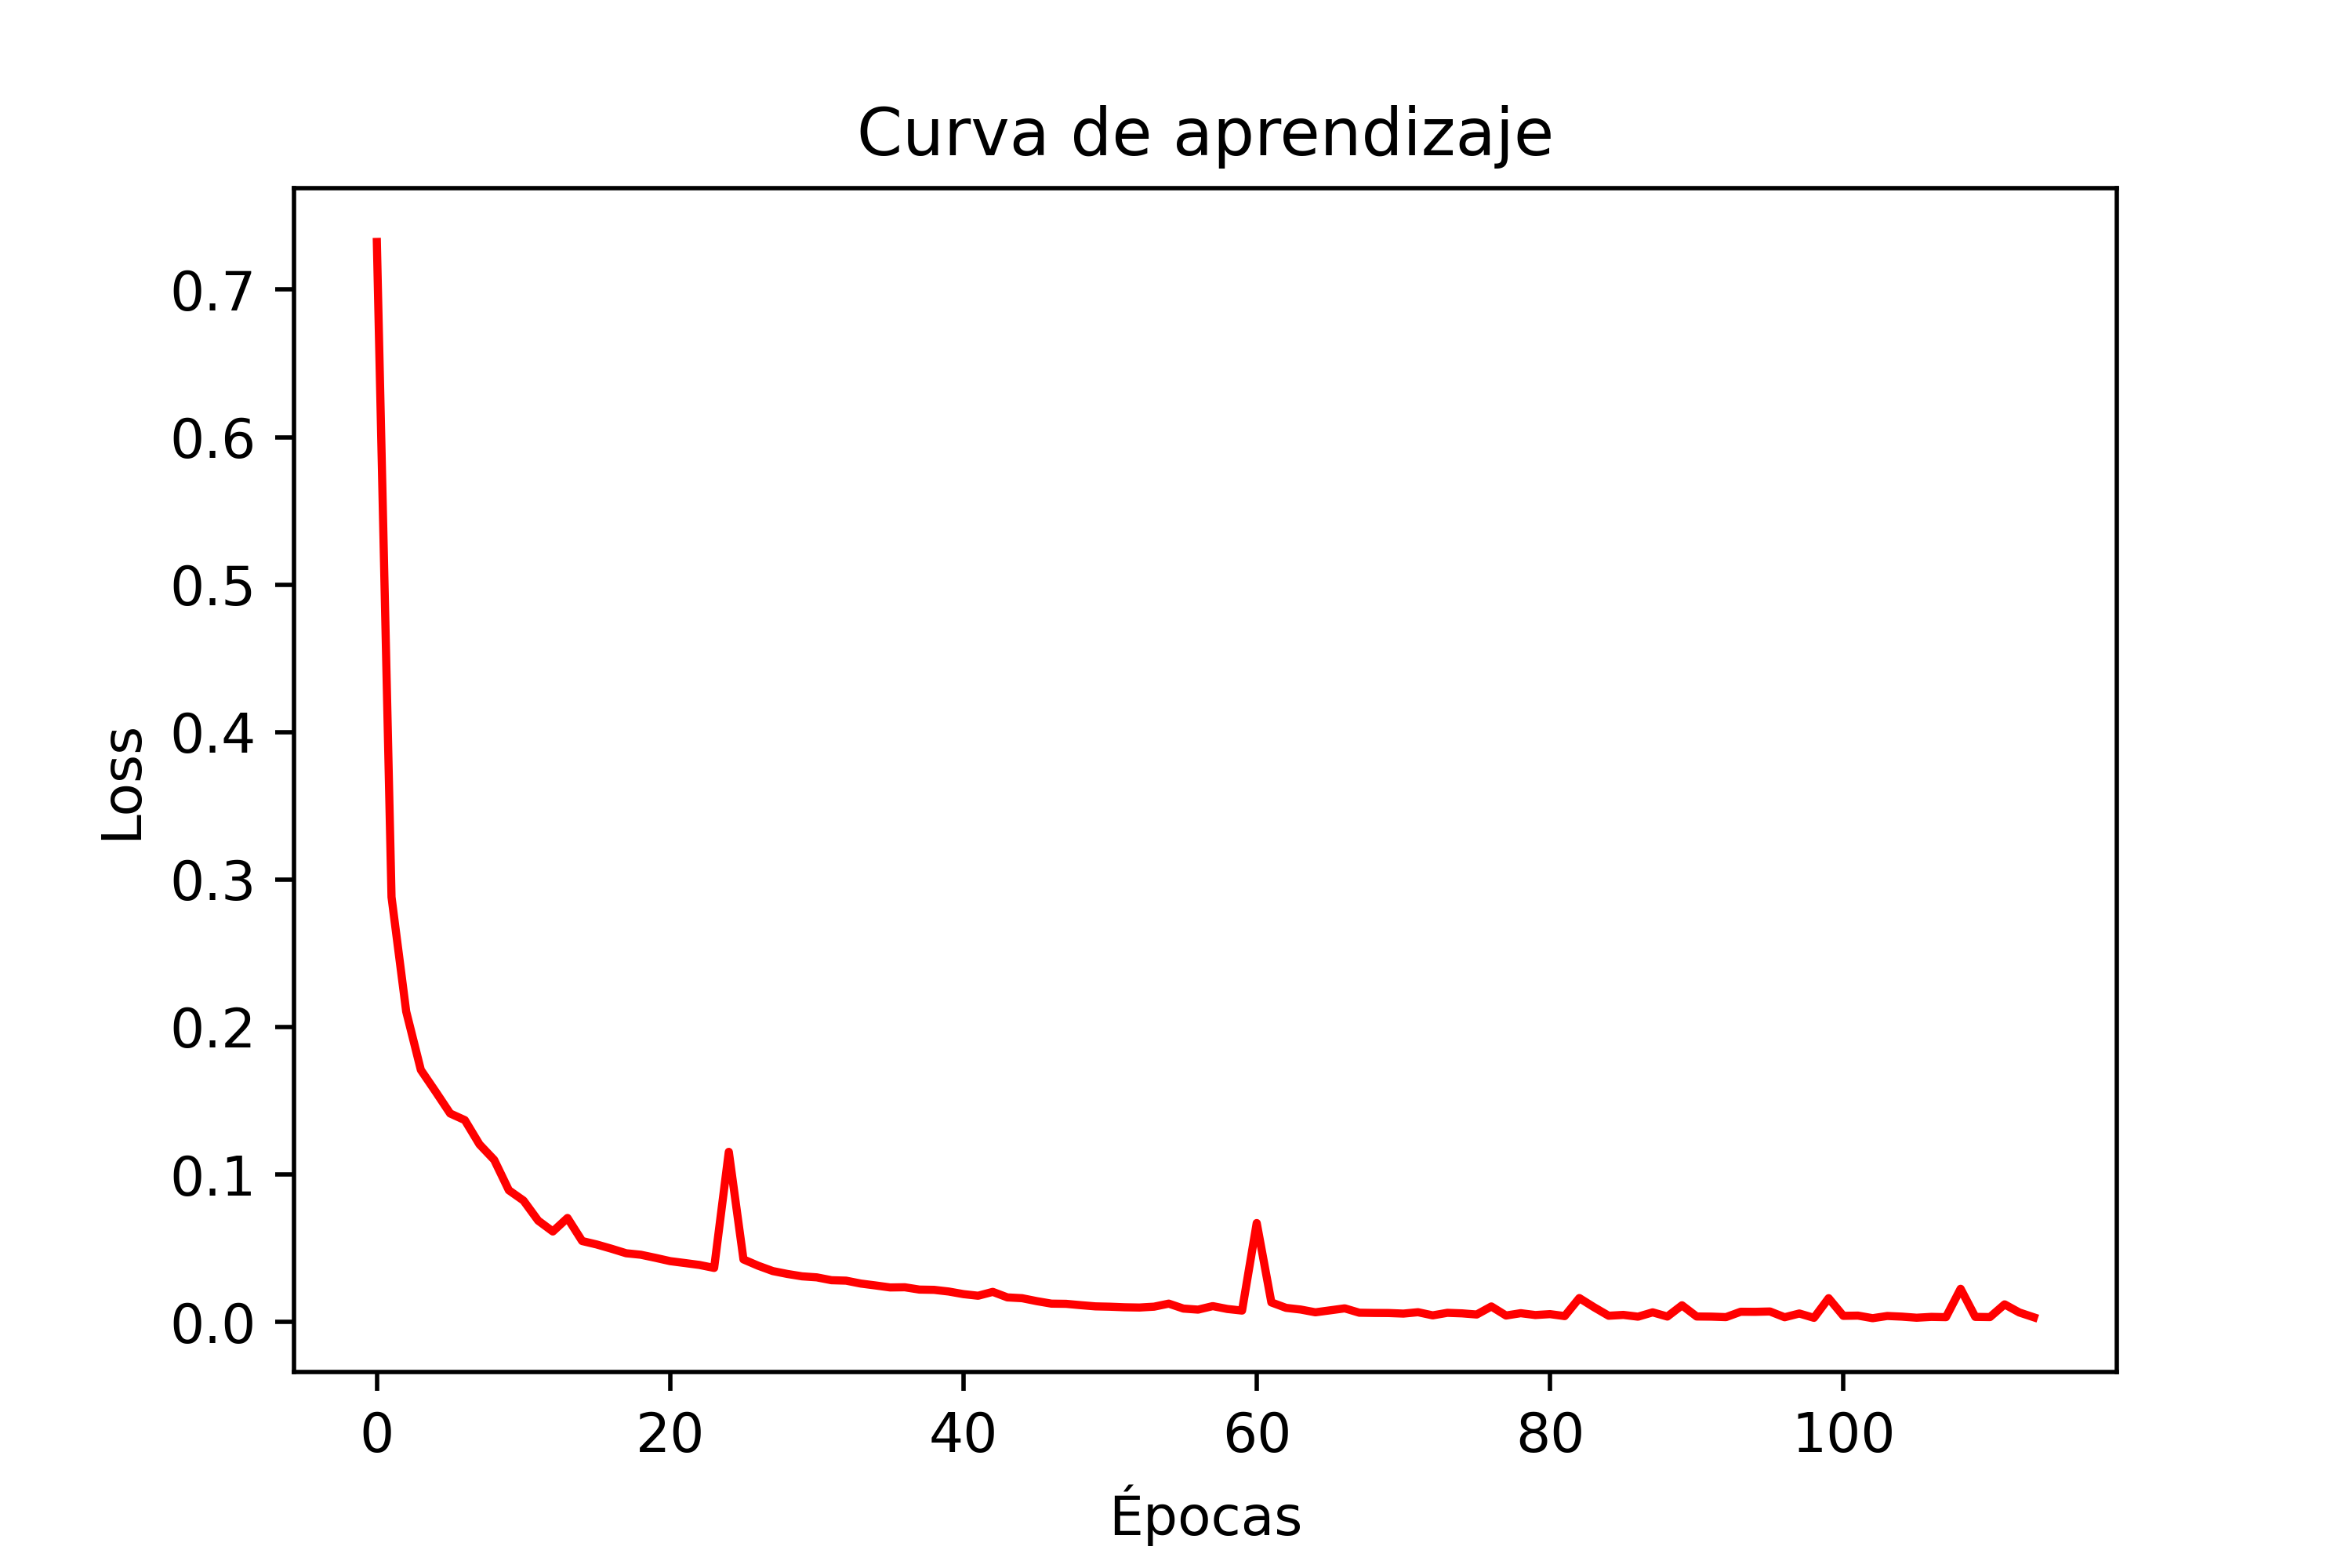
\includegraphics[scale=0.71]{imgss189.png}
	\caption{Resultado 14.}
	\label{fig:figura1000_39}
\end{figure} 

El resultado de la \autoref{fig:figura1000_39} corresponde a una red neuronal con 2 capas ocultas, 20 nodos en cada capa y un valor de 0.2 como tasa de aprendizaje. La función de activación utilizada para las capas ocultas es la 
función tangente hiperbólica y logra un porcentaje de aciertos de 100$\%$ en validación después de ejecutar 114 épocas de entrenamiento. En este caso particular, nuevamente la función de costo no logró llegar al valor de 0 
durante la fase de entrenamiento. Sin embargo, para la fase de validación del modelo, la optimización para los pesos dada por el entrenamiento logró acertar en el total de estimaciones posibles. 

Para este caso particular, se puede observar como en la curva de entrenamiento de minimización del error existen partes donde se tienen salto bruscos en los cuales la magnitud de la función de costo se incrementa rápidamente 
en pocas épocas, y después se estabiliza nuevamente. Este tipo de comportamiento es normal debido a que el método de optimización de descenso por gradiente en un punto específico del entrenamiento puede generar pasos de 
magnitud elevada pero en dirección opuesta a la requerida, es decir, el error crece. Este tipo de tendencia se puede evitar principalmente haciendo cambios en el valor de tasa de aprendizaje, lo cual genera que los pasos 
dados por el algoritmo sean más pequeños.

En la \autoref{fig:figura1000_42} se tiene un caso similar.


\begin{figure}[h]
	\centering
	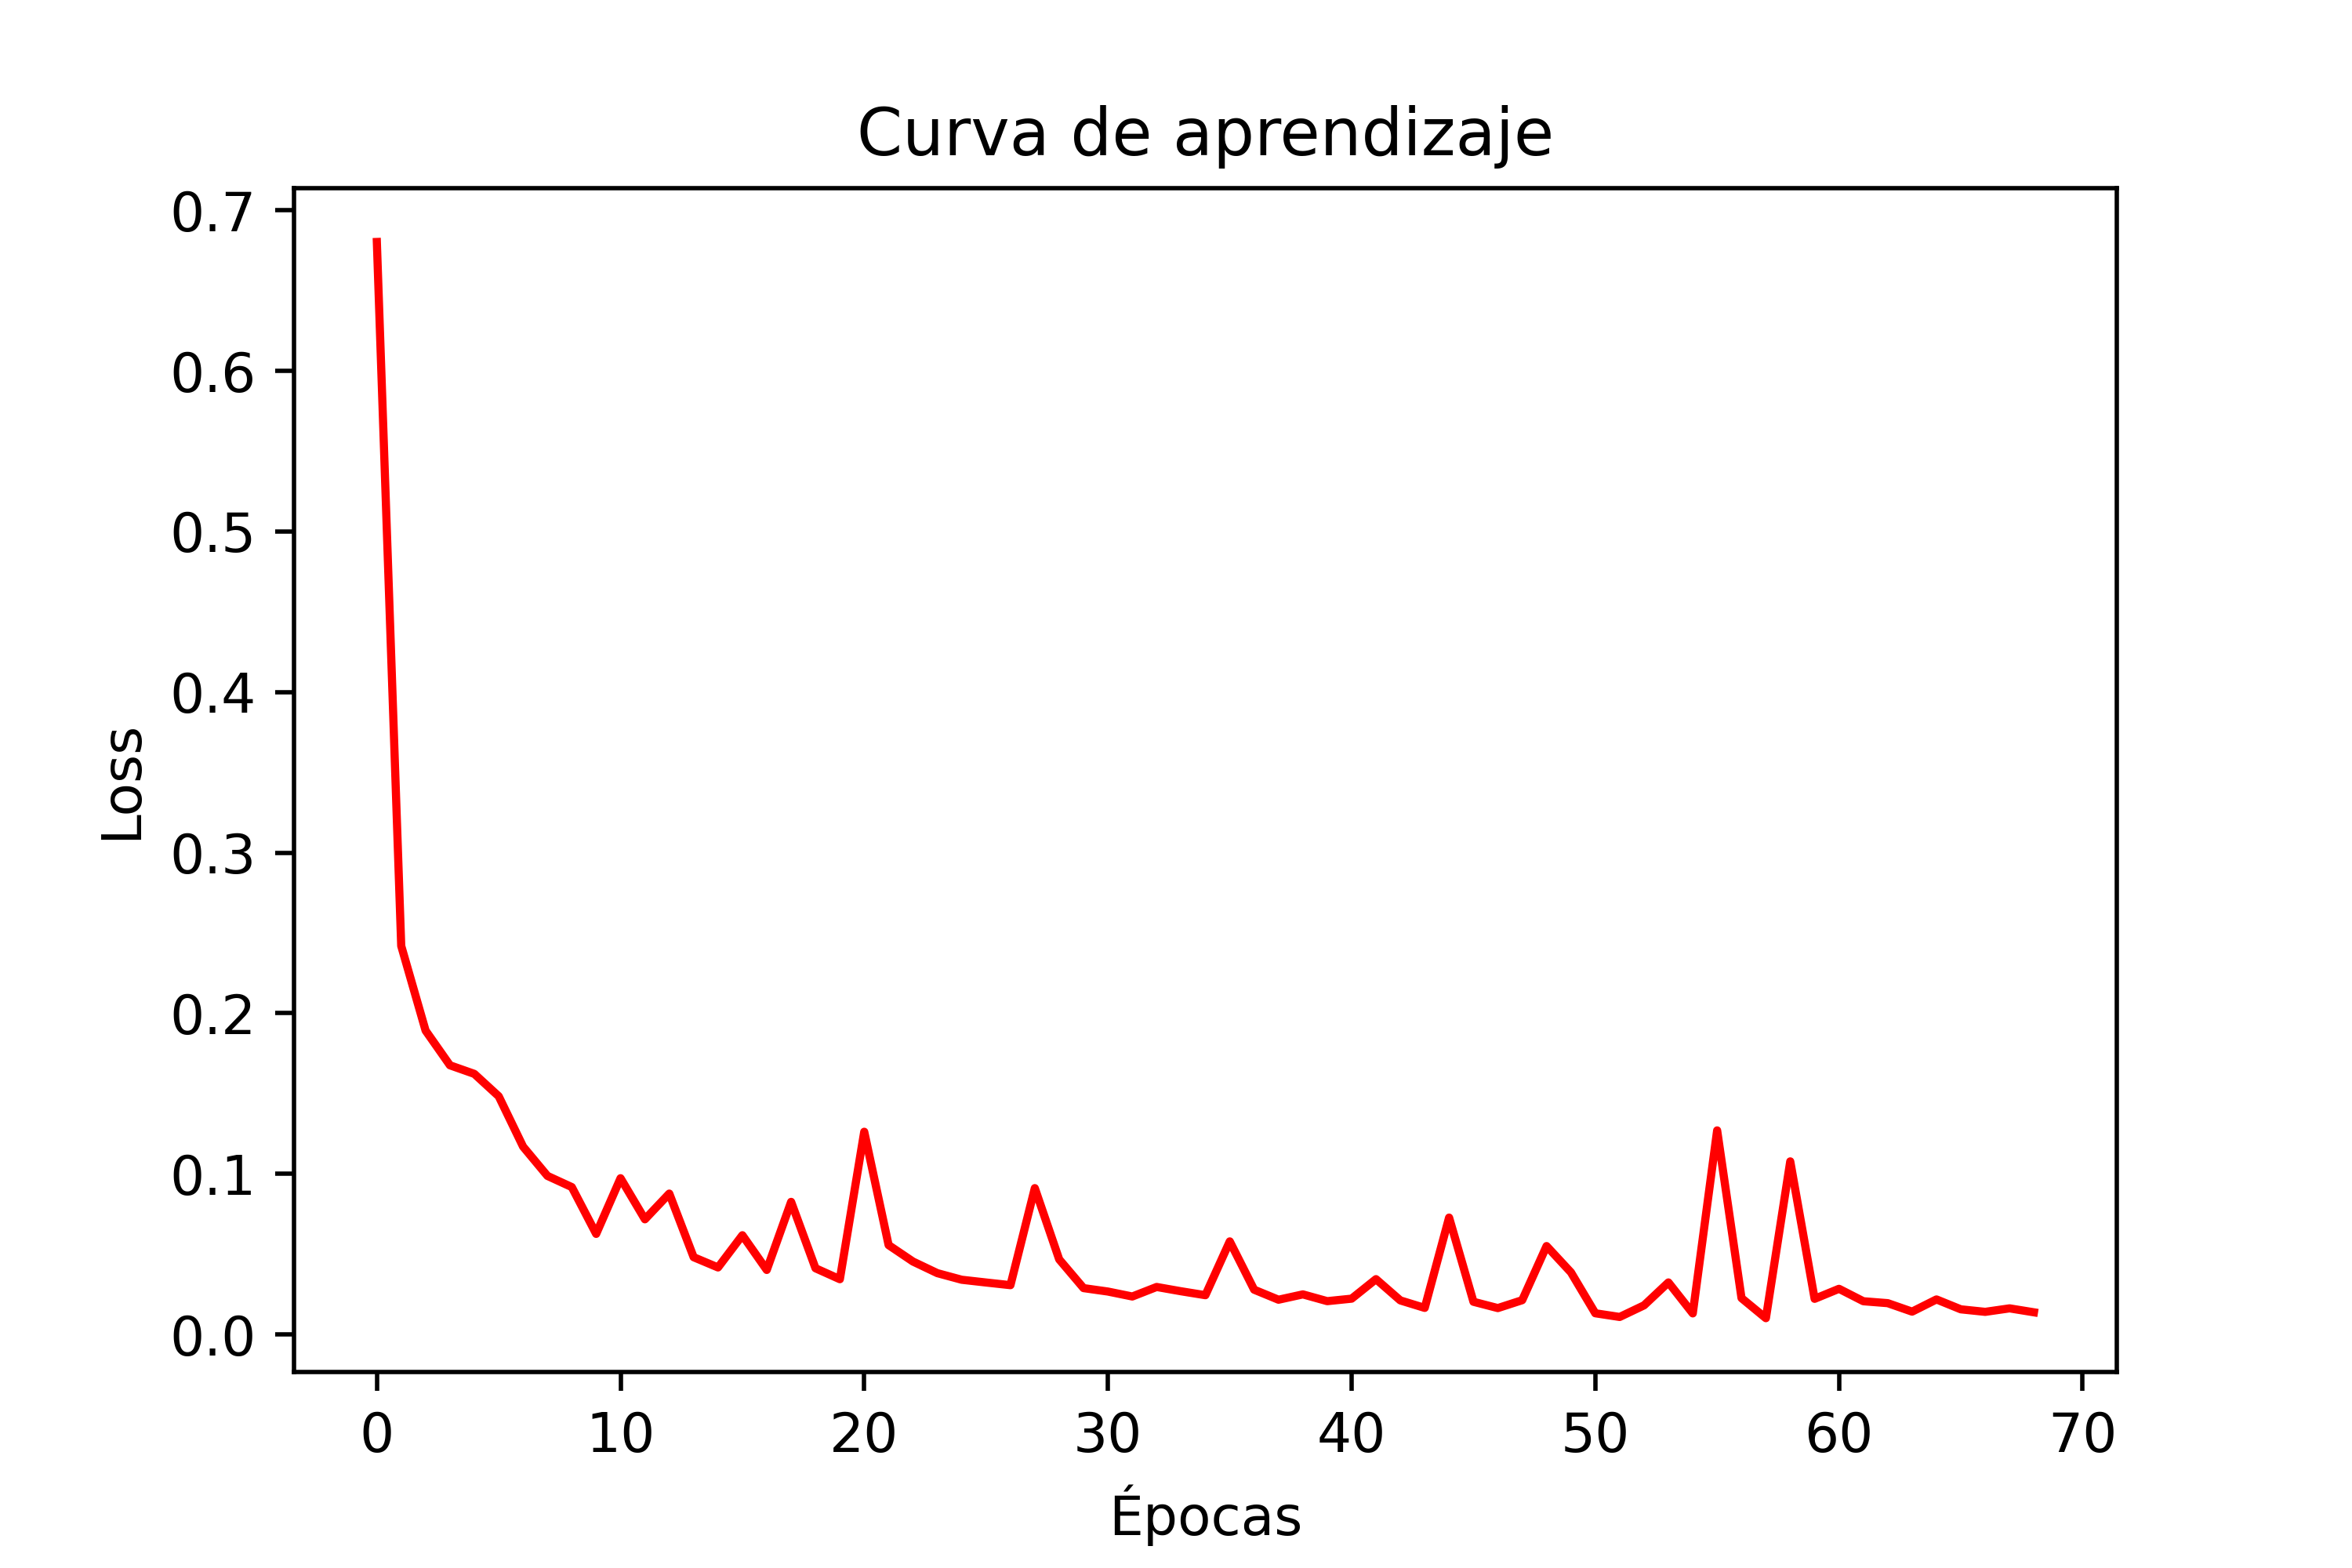
\includegraphics[scale=0.71]{imgss192.png}
	\caption{Resultado 17.}
	\label{fig:figura1000_42}
\end{figure} 

Este resultado se logra con una red neuronal de 2 capas ocultas, 30 nodos en cada capa y un valor de 0.3 de tasa de aprendizaje. La función de activación utilizada es la función tangente hiperbólica y se logra un porcentaje 
de aciertos de 100$\%$ en validación después de ejecutar 69 épocas de entrenamiento. 

Finalmente, de los resultados dados por la \autoref{tab:table200_1}, es evidente que los casos en los cuales el modelo emplea 2 capas de ocultas, decrece de forma considerable el número de épocas en entrenamiento necesarias 
para la convergencia en la minimización del error. Este comportamiento cumple con la expectativa ya que al tener más nodos al agregar otra capa oculta, los patrones que puede generar la red neuronal pueden ser más complejos 
y eso ayuda a reducir el número de iteraciones requeridas a través de todo el conjunto de datos de entrenamiento. 

\clearpage

\subsection{Resultados para conjunto principal de datos. Entrenamiento con 70$\%$ de los datos}

Con el conjunto principal de datos del proceso de potabilización se mostró en la sección \textit{6.3.1 Resultados para conjunto principal de datos}, los resultados de clasificación con redes neuronales usando un 80$\%$ de 
los datos como conjunto para entrenamiento y el 20$\%$ restante como conjunto para pruebas de validación. En esta sección se muestran los resultados de pruebas de validación similares pero usando 70$\%$ del total de datos 
para entrenamiento y 30$\%$ para validación. El reducir la cantidad de datos usados en entrenamiento ayuda a evitar sobreentrenamiento de la red neuronal, además de que permite tener un clasificador que pueda adaptarse de 
mejor manera en pruebas adicionales con datos que no provengan del conjunto recolectado. Es decir entre mayor sea el porcentaje de datos de entrenamiento, el modelo clasificador estará mejor ajustado u optimizado para el 
conjunto específico de datos con los que yo cuento, pero posiblemente con otro conjunto de datos ajeno los resultados del porcentaje de aciertos del clasificador sea más bajo debido a que el modelo esta sobreajustado a la 
tendencia dada por los datos que yo he recolectado.

En la \autoref{tab:table200_2} se muestran los resultados con mayor porcentaje de aciertos, así como la arquitectura empleada.

\begin{table}[h]
	\begin{center}
		\begin{tabular}{| c | c | c | c | c |}
	    	\hline
            Nodos en capas ocultas & Tasa de aprendizaje & Épocas & Función de activación & Aciertos \\ \hline
			(20,20) & 0.1 & 150 & tanh & 100\% \\
			(30,30) & 0.2 & 93 & tanh & 99.77\% \\
			5 & 0.25 & 244 & Sigmoide & 94.28\% \\
			5 & 0.25 & 156 & tanh & 95.63\% \\
			8 & 0.25 & 797 & Sigmoide & 97.85\% \\
			8 & 0.25 & 283 & tanh & 98.09\% \\
			10 & 0.25 & 270 & Sigmoide & 95.01\% \\
			10 & 0.25 & 258 & tanh & 97.5\% \\
			15 & 0.25 & 733 & Sigmoide & 98.33\% \\
			15 & 0.25 & 306 & tanh & 98.9\% \\ \hline
	    \end{tabular}	
		\caption{Resultados de validación con 70$\%$ de datos para entrenamiento.}
        \label{tab:table200_2}	
	\end{center}
\end{table}

Con estos resultados se tiene evidencia de que un 70$\%$ de datos de entrenamiento es suficiente para lograr que la red neuronal se ajuste adecuadamente a la tendencia dada por el conjunto de datos empleado para validación.

\clearpage

\subsection{Resultados de clasificación con datos atípicos}

El conjunto principal de datos recolectados se compone de 16434 registros, cada uno de ellos con 3 elementos dados por 3 parámetros, ORP, cloro residual y oxígeno disuelto. Si se agregan los datos muestreados durante el 
mes de agosto el conjunto crece a 18454 registros, igualmente cada uno de ellos con 3 valores cada registro. Es ahora con este conjunto más amplio de datos que se presentan los resultados para clasificación con el fin de observar 
el efecto sobre los porcentajes de acierto y minimización de la función de costo si los datos atípicos forman parte del entrenamiento de la red neuronal y posteriormente de la validación.

\begin{table}[h]
	\begin{center}
		\begin{tabular}{| c | c | c | c | c |}
	    	\hline
            Nodos en capas ocultas & Tasa de aprendizaje & Épocas & Función de activación & Aciertos \\ \hline
			(20,20) & 0.1 & 150 & tanh & 99.71\% \\
			(30,30) & 0.2 & 90 & tanh & 98.37\% \\
			5 & 0.25 & 244 & Sigmoide & 88.83\% \\
			5 & 0.25 & 156 & tanh & 90.98\% \\
			8 & 0.25 & 327 & Sigmoide & 93.55\% \\
			8 & 0.25 & 150 & tanh & 95.84\% \\
			10 & 0.25 & 270 & Sigmoide & 95.05\% \\
			10 & 0.25 & 146 & tanh & 95.68\% \\
			15 & 0.25 & 373 & Sigmoide & 96.36\% \\
			15 & 0.25 & 306 & tanh & 98.26\% \\ \hline
	    \end{tabular}	
		\caption{Resultados de validación para datos atípicos con 70$\%$ de datos para entrenamiento.}
        \label{tab:table200_3}	
	\end{center}
\end{table}

En la \autoref{tab:table200_3} el porcentaje de aciertos alcanzado indica que a pesar de hay un pequeño descenso al trabajar con las arquitecturas que han dado mejores resultados previamente y no se logra llegar a 100$\%$ 
de clasificación correcta, aún así el modelo de red neuronal sigue adaptándose adecuadamente a pesar de que en entrenamiento y validación ahora se incluyeron registros de datos con patrones de comportamiento contradictorios 
en comparación a los resultados anteriores.

A continuacion se muestran gráficas con las curvas de entrenamiento para la minimización de la función de costo con las arquitecturas empledas en la \autoref{tab:table200_3}.

\clearpage

\begin{figure}[h]
	\centering
	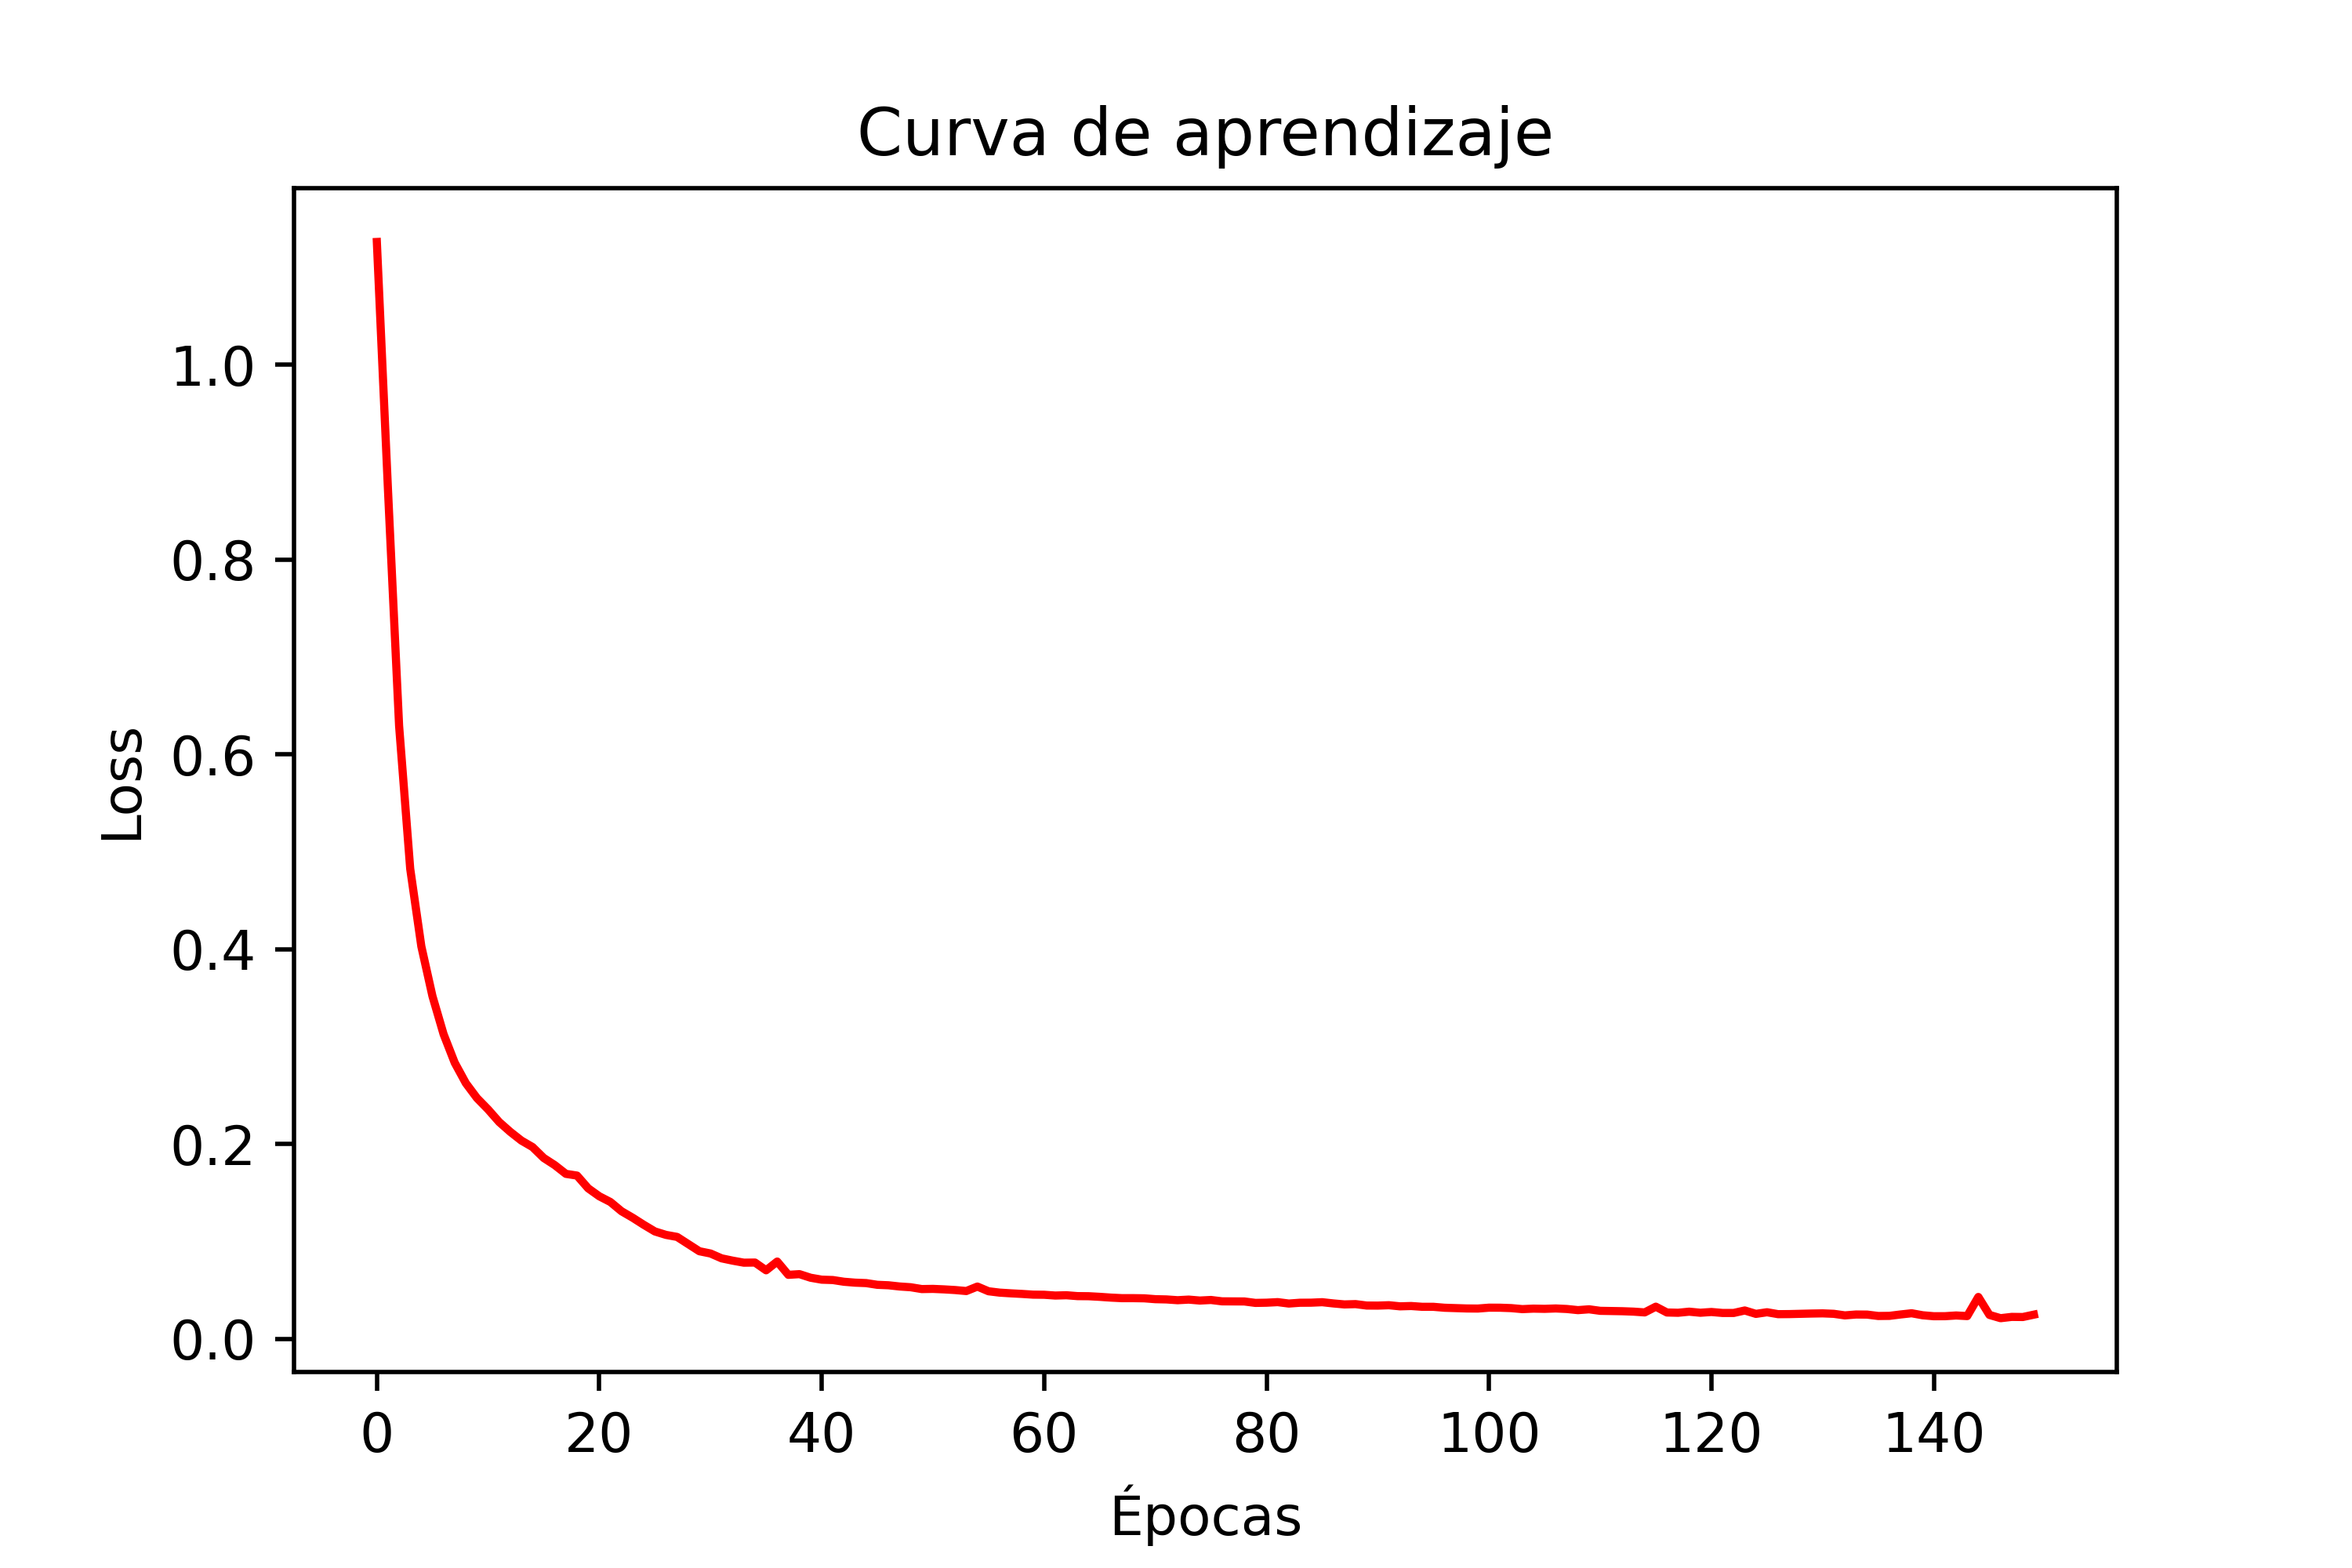
\includegraphics[scale=0.71]{imgss193.png}
	\caption{Resultado 1.}
	\label{fig:figura1000_43}
\end{figure}

El resultado de la \autoref{fig:figura1000_43} corresponde a una red neuronal con 2 capas ocultas, 20 nodos en cada capa y un valor de 0.1 como tasa de aprendizaje. La función de activación utilizada para las capas ocultas es la 
función tangente hiperbólica y logra un porcentaje de aciertos de 99.71$\%$ para validación después de ejecutar 150 épocas en entrenamiento. 
Para esta ejemplo particular no se logra la convergencia a un valor de 0 para la función de error, sin embargo con aproximadamente 50 épocas de optimización el modelo ya ha alcanzado un valor cercano al punto de convergencia 
para la minimización. Por lo tanto, a pesar de la inclusión de los datos atípicos del mes de agosto, este tipo de algoritmo sigue presentando una eficiencia adecuada a pesar de introducir en el entrenamiento valores que no 
corresponden con la tendencia general de los datos. 

\begin{figure}[h]
	\centering
	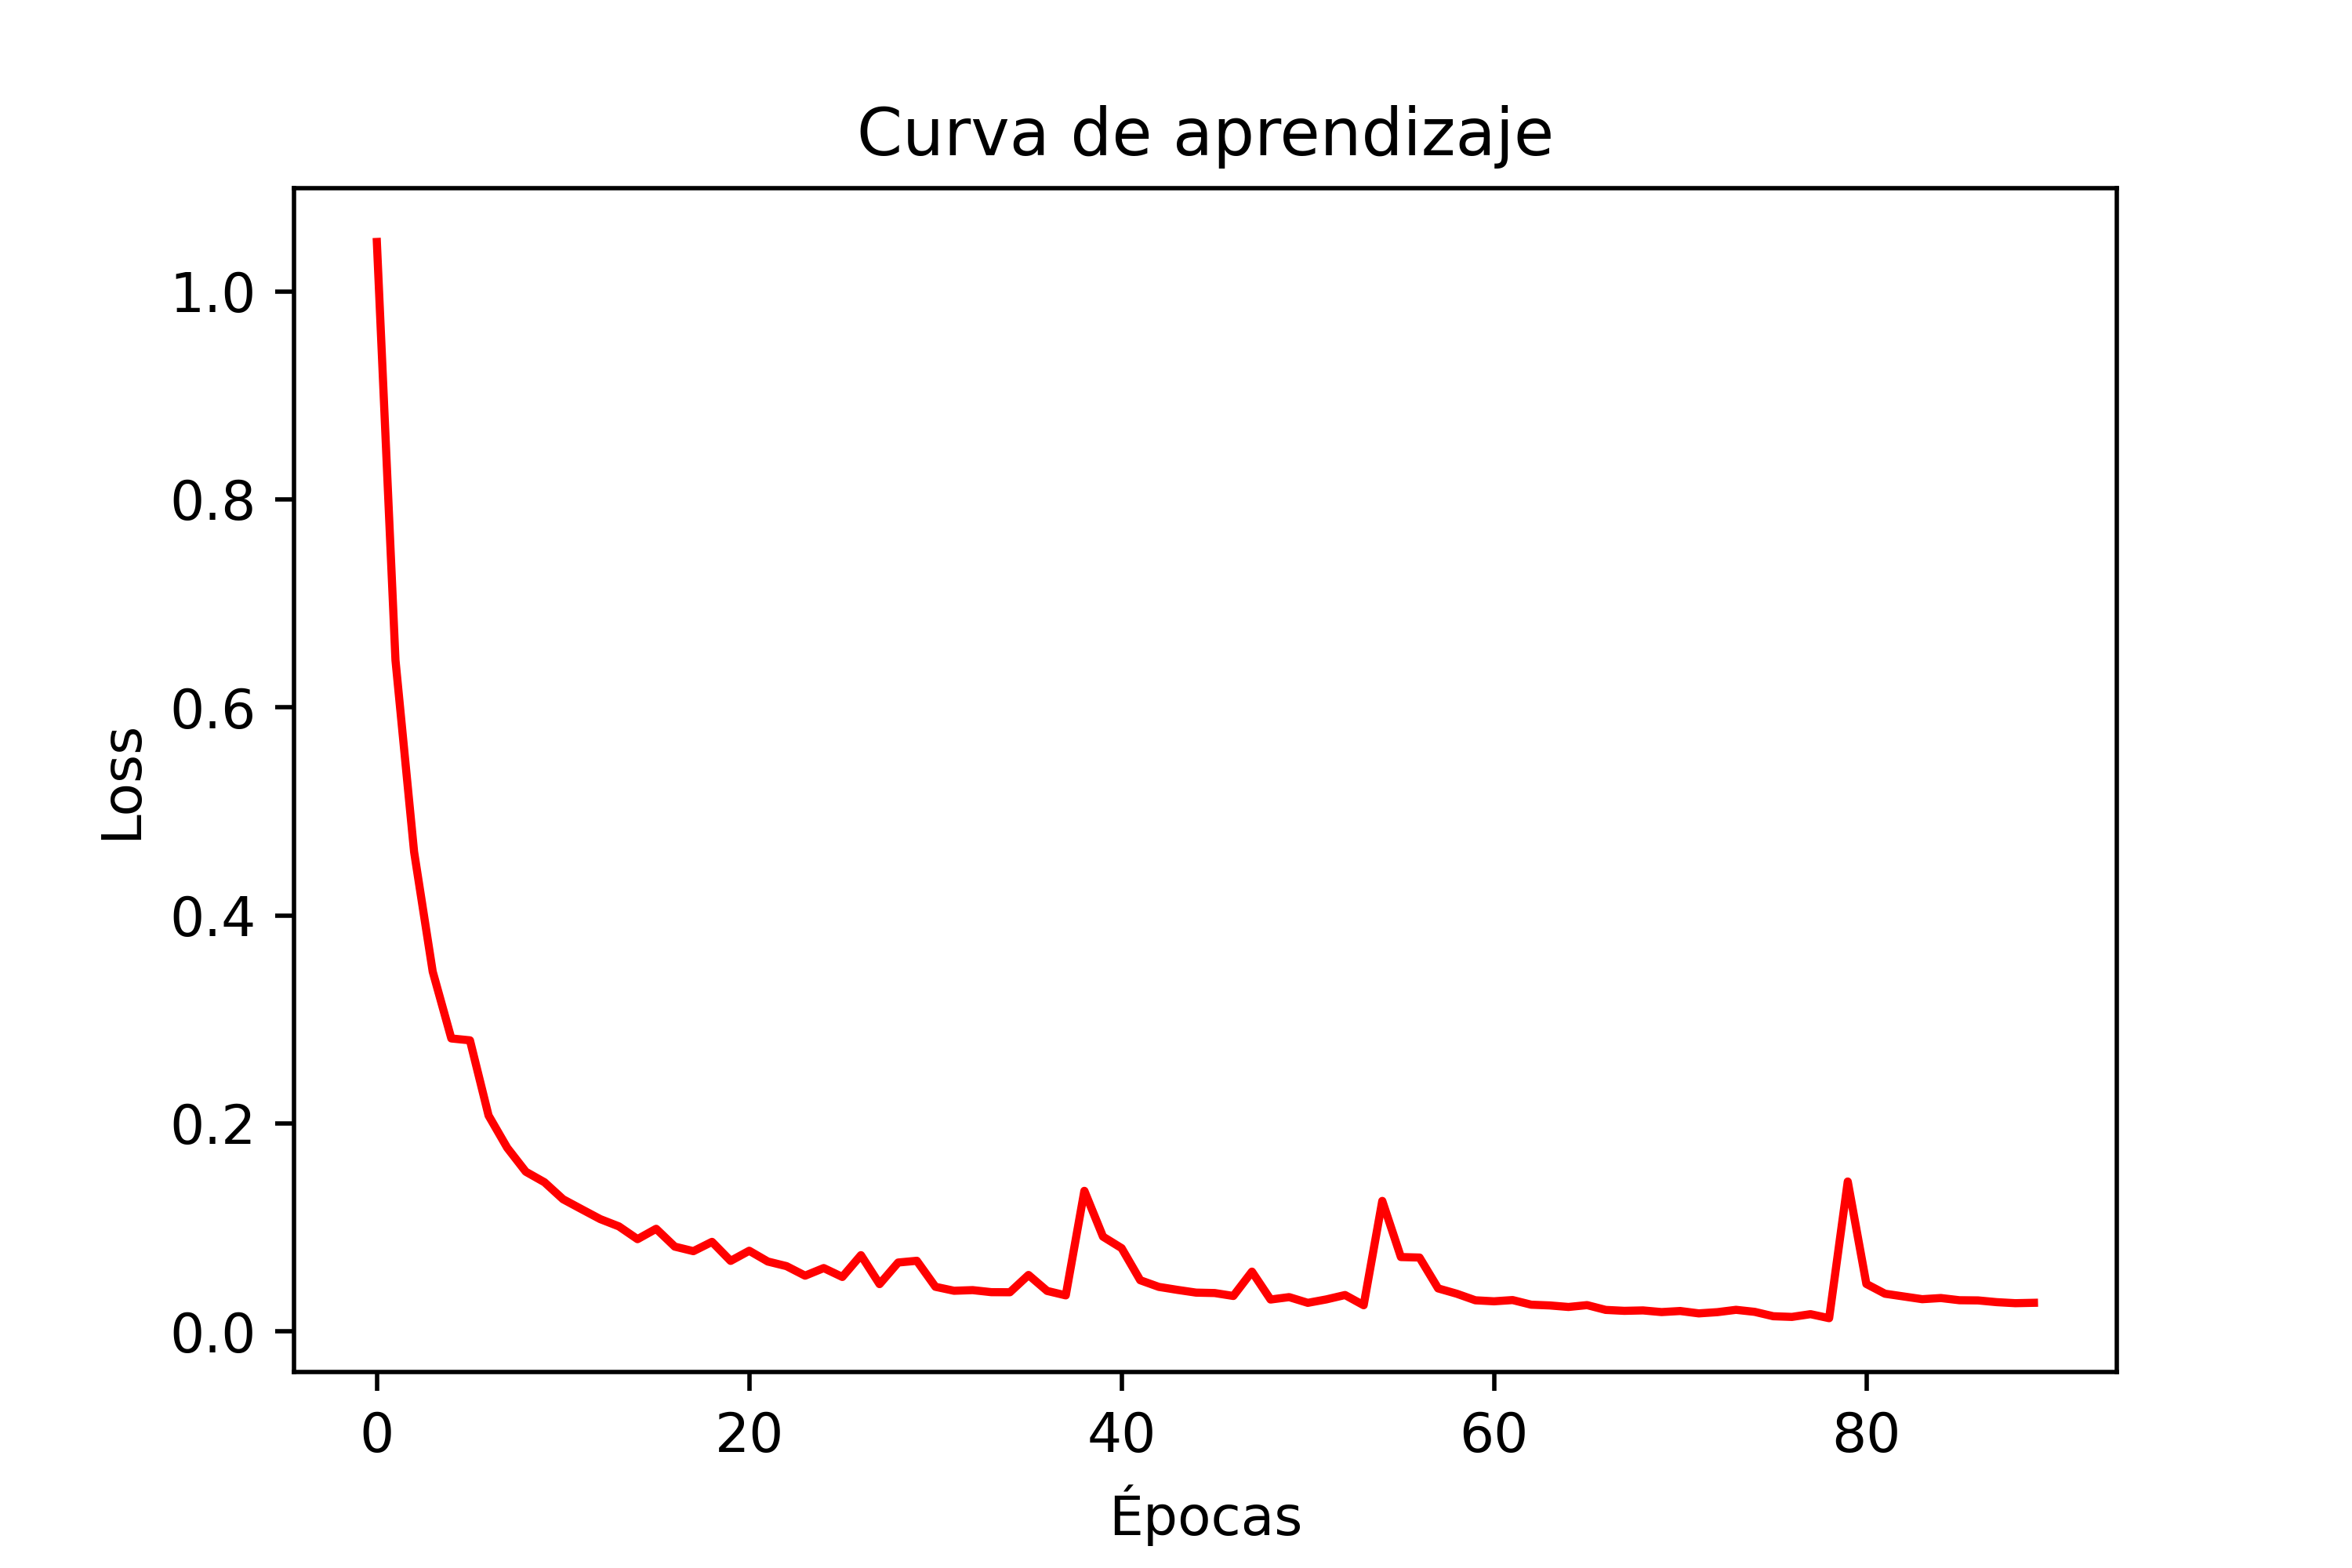
\includegraphics[scale=0.71]{imgss194.png}
	\caption{Resultado 2.}
	\label{fig:figura1000_44}
\end{figure}

\clearpage

El resultado de la \autoref{fig:figura1000_44} corresponde a una red neuronal con 2 capas ocultas, 30 nodos en cada capa y un valor de 0.2 como tasa de aprendizaje. La función de activación utilizada para las capas ocultas es la 
función tangente hiperbólica y logra un porcentaje de aciertos de 98.37$\%$ después de ejecutar 90 épocas de entrenamiento.
La parte a resaltar con este ejemplo es que si se hace la comparación con el resultado de la \autoref{fig:figura1000_43}, en este nuevo ejemplo al agregar 10 nodos en cada capa oculta y elevar a 0.2 la tasa de aprendizaje, 
se logra reducir de 150 a 90 el número de épocas de entrenamiento necesarias para la convergencia en la minimización de la función de costo.

\section{Conclusiones}

En este capítulo se ha presentado una descripción temporal sobre las diferentes toma de muestras realizadas en la planta de potabilización, haciendo énfasis en los resultados puntuales para cada caracterización, así como 
también en las diversas modificaciones que se tuvieron que realizar para optimizar y mejorar las medición para la generación de nuestra base de datos.

Posteriormente se han presentado las evidencias estadísticas donde se exponen los argumentos en los cuales se ha basado para la elección de las variables de calidad del agua que serían utilizadas para el algoritmo de clasificación, 
así como también la evidencia que sustenta la exclusión de los parámetros de temperatura, pH y conductividad.

Finalmente, se exponen los resultados para el modelo de clasificación por red neuronal, en los cuales se dividen las evidencias en subsecciones para resaltar que se puede generar un desempeño adecuado y eficiente con este 
tipo de modelo. Se hicieron pruebas utilizando como conjunto de datos de entrenamiento el 80$\%$ del total de datos, también con únicamente el 70$\%$, así como también con la adición de los registros correspondientes al 
mes de agosto de datos atípicos. A pesar de tener diferentes escenarios para la optimización de la red neuronal, el modelo ha logrado adaptarse a los datos que se le introducen, generando alto desempeño en las pruebas de 
validación.

\clearpage
